In this section, we investigate the identification of boosted top quarks using jet substructure. Boosted top quarks result in large-radius jets with complex substructure, containing a $b$-subjet and a boosted $W$. As a consequence of the many kinematic differences between top and QCD jets, top taggers are typically complex, with a couple of input parameters necessary for any given algorithm. We study the variation in performance of top tagging techniques with respect to jet \pt and $R$, re-optimizing the tagger inputs for each kinematic range and jet radius considered. We also investigate the effects of combining dedicated top tagging algorithms with other jet substructure variables, giving insight into the correlations among top-tagging variables.


\subsection{Methodology}\label{sec:topmethod}

We use the top quark MC samples for each bin described in Section \ref{sec:top-samples}. The analysis  relies on \textsc{FastJet} 3.0.3 for jet clustering and
calculation of jet substructure variables. Jets are clustered using the \antikt algorithm, and only the leading jet is used in each analysis. To ensure similar $\pt$ spectra in each bin an upper and lower $\pt$ cut are applied to each sample after jet clustering. The bins in leading jet $\pt$
 for top tagging are 600-700 \GeV, 1-1.1 \TeV, and
1.5-1.6 TeV. Jets are clustered with radii $R=0.4$, 0.8, and 1.2; $R=0.4$ jets are only studied in the 1.5-1.6 TeV bin
because the top decay products are all contained within an $R=0.4$ jet for top quarks with this boost.

We study a number of top-tagging strategies, which can be divided into two distinct categories. In the first category are dedicated top-tagging algorithms, which aim to directly reconstruct the top and $W$ candidates in the top decay. In particular, we study:
%
\begin{enumerate}
\item HEPTopTagger
\item Johns Hopkins Tagger (JH)
\item Trimming with $W$-identification
\item Pruning with $W$-identification
\end{enumerate}
%
as described in Section~\ref{sec:taggers}. 
In the case of the HepTopTagger and JH tagger, the algorithms produce three output variables ($\topmass$, $\wmass$ and helicity angle) that can be used to discriminate top jets from QCD. The trimming and pruning algorithms as used here produce two outputs, $\topmass$ and $\wmass$. All of the above taggers and groomers incorporate a step to remove contributions from the underlying event and other soft radiation to the reconstructed $\topmass$ and $\wmass$, and also explicitly rejects jets that do not meet basic selection criteria, as explained in detail in Section~\ref{sec:taggers}.

In the second category are individual jet substructure variables that are sensitive to the radiation pattern within the jet, which we refer to as ``jet-shape variables''. While the most sensitive top-tagging variables are typically sensitive to three-pronged radiation, we also consider variables sensitive to two-pronged radiation in the limit where the $W$ is very boosted and its subjets overlap. The variables we consider are:
%
\begin{itemize}
\item The ungroomed jet mass.
\item $N$-subjettiness ratios \tautwoone and \tauthreetwo, using the ``winner-takes-all'' axes definition.
\item 2-point energy correlation function ratios $C_2^{\beta=1}$ and $C_3^{\beta=1}$.
\item The pruned Qjet mass volatility, $\Gamma_{\rm Qjet}$.
\end{itemize}
%
Several of these variables were also considered earlier for $q/g$-tagging and $W$-tagging.

To study the correlations amongst the above substructure variables and tagging algorithms,
we combine the relevant tagger output variables and/or jet shapes into a BDT\footnote{Similar studies were recently performed for the HepTopTagger in~\cite{Kasieczka:2015jma}, in the context of trying to improve the tagger by combining it's outputs with $N$-subjettiness and Qjet mass volatility}, as described in Section~\ref{sec:multivariate}. 
Additionally, because each tagger has two input parameters, we scan over reasonable values of the input parameters to determine the optimal value that gives the largest background rejection for each top tagging signal efficiency. This allows a direct comparison of the optimized version of each tagger. The input parameter values scanned for the various algorithms are:
%
\begin{itemize}
\item {\bf HEPTopTagger:} $m\in[30,100]$ \GeV, $\mu\in[0.5,1]$
\item {\bf JH Tagger:} $\delta_p\in[0.02,0.15]$, $\delta_R\in[0.07,0.2]$
\item {\bf Trimming:} $f_{\rm cut}\in[0.02,0.14]$, $R_{\rm trim}\in[0.1,0.5]$
\item {\bf Pruning:} $z_{\rm cut}\in[0.02,0.14]$, $R_{\rm cut}\in[0.1,0.6]$
\end{itemize}
%
We also investigate the degradation in performance of the top-tagging variables when moving away from the optimal parameter choice.

\subsection{Single Variable Performance}\label{sec:single_variable}
We begin by investigating the behaviour of individual jet substructure variables. Because of the rich, three-pronged structure of the top decay, it is expected that combinations of masses and jet shapes will far outperform single variables in identifying boosted tops. However, a study of the top-tagging performance of single variables facilitates a direct comparison with the $W$ tagging results in Section \ref{sec:wtagging}, and also allows a straightforward examination of the performance of each variable for different $\pt$ and jet radius.

Top-tagging performance is quantified using ROC curves. Figure~\ref{fig:single_variable_ROC} shows the ROC curves for each of the top-tagging variables, with the bare (ungroomed) jet mass also plotted for comparison. The jet-shape variables all perform substantially worse than ungroomed jet mass; this is in contrast with $W$ tagging, for which several variables are competitive with or perform better than ungroomed jet mass (see, for example, Figures~\ref{fig:pt500_comb2D_08}, \ref{fig:pt1000_comb2D_04} and~\ref{fig:pt1000_comb2D_08}).
To understand why this is the case, consider $N$-subjettiness:~the $W$ is two-pronged and the top is three-pronged, and so we expect $\tau_{21}$ and $\tau_{32}$ to be the best-performant $N$-subjettiness ratios, respectively. However, a cut selection small values of $\tau_{21}$ necessarily selects for events with large $\tau_1$, which is strongly correlated with jet mass, up to exponentially suppressed contributions. Therefore, $\tau_{21}$ applied to $W$-tagging indirectly incorporates some information about the jet mass in addition to shape information. By contrast, $\tau_{32}$ applied to top tagging does not include any information on the ungroomed jet mass information.  This likely accounts for why, relative to a cut on ungroomed mass, $\tau_{32}$ for top tagging performs substantially worse than $\tau_{21}$ for $W$-tagging. 


\begin{figure*}
\centering
\subfigure[Jet shapes]{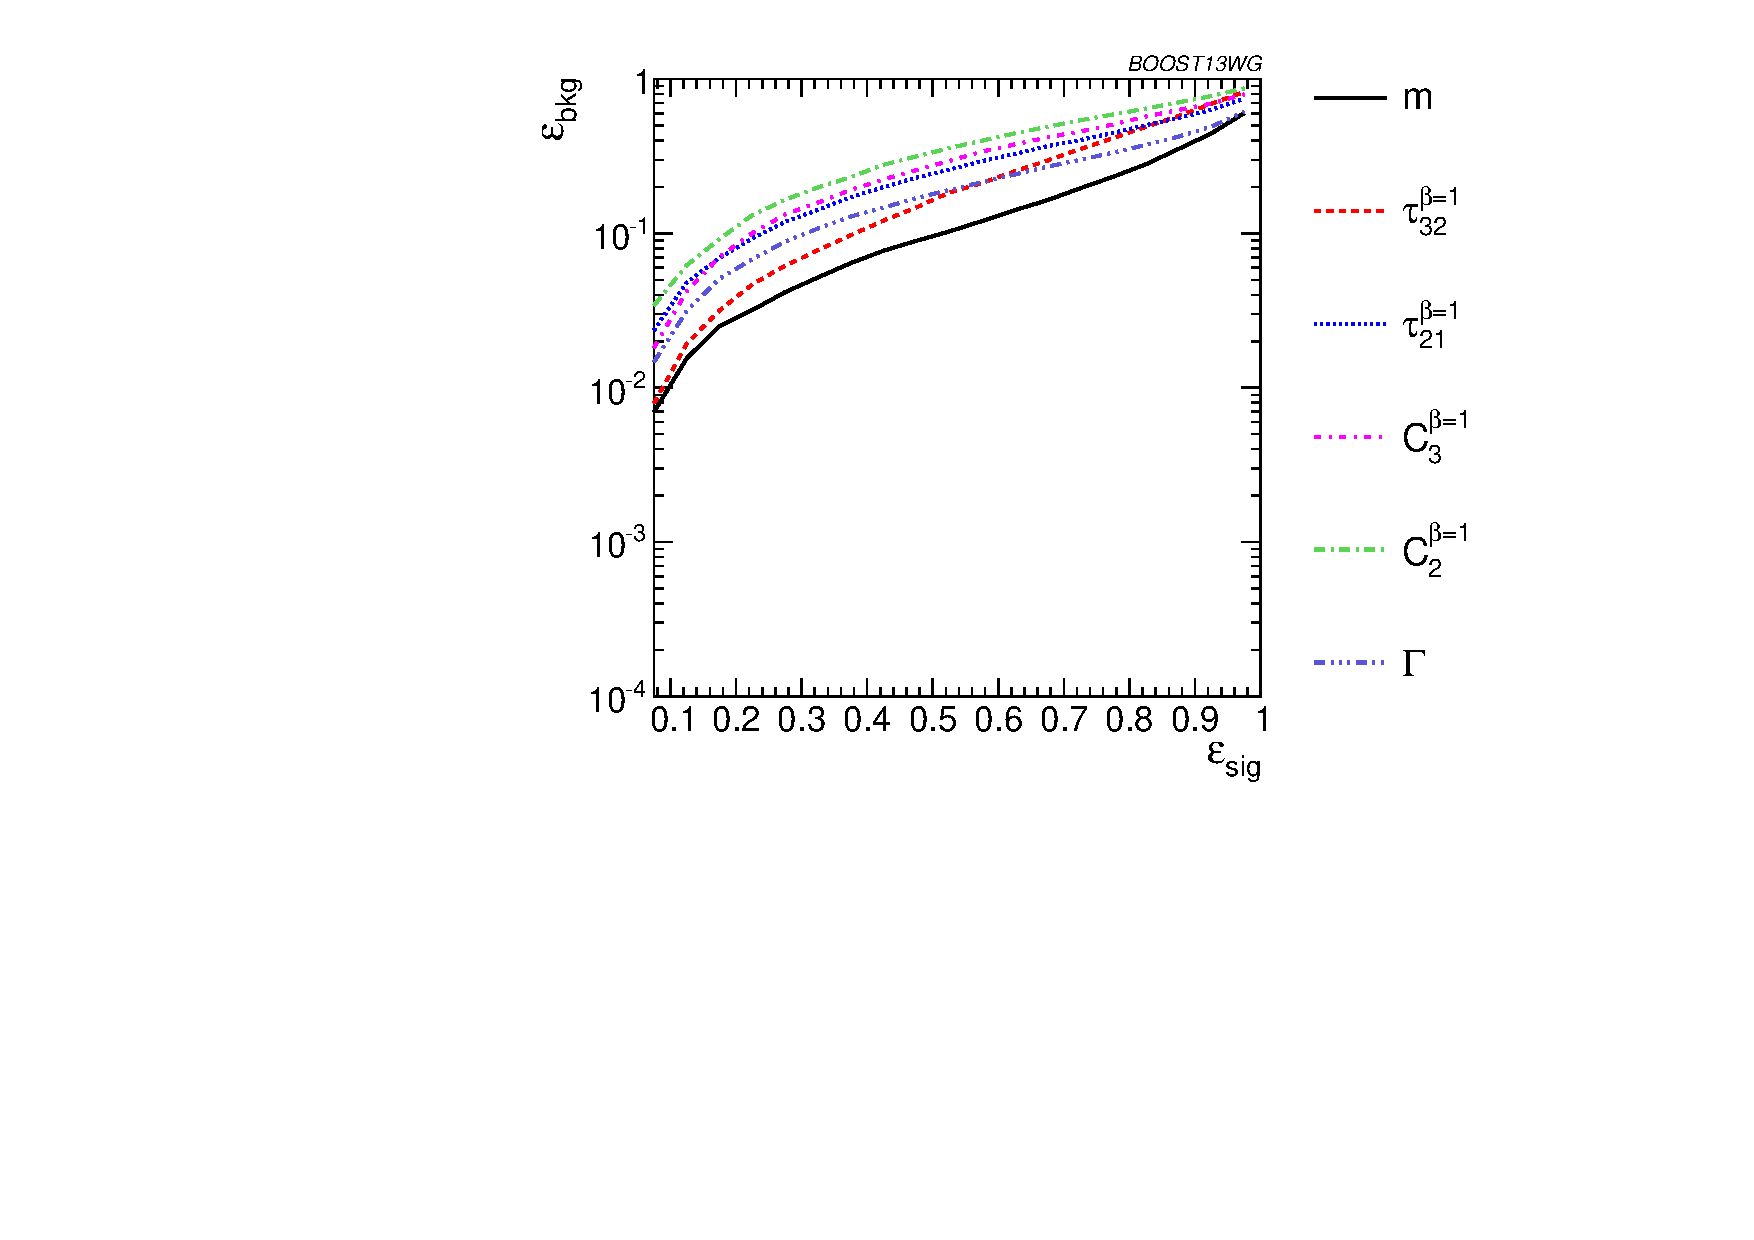
\includegraphics[width=0.49\textwidth]{./Figures/TTagging/single_variable/pT.1TeV.R.0.8/Rocs_shape.pdf}\label{fig:single_variable_ROC_shape}}
\subfigure[top mass]{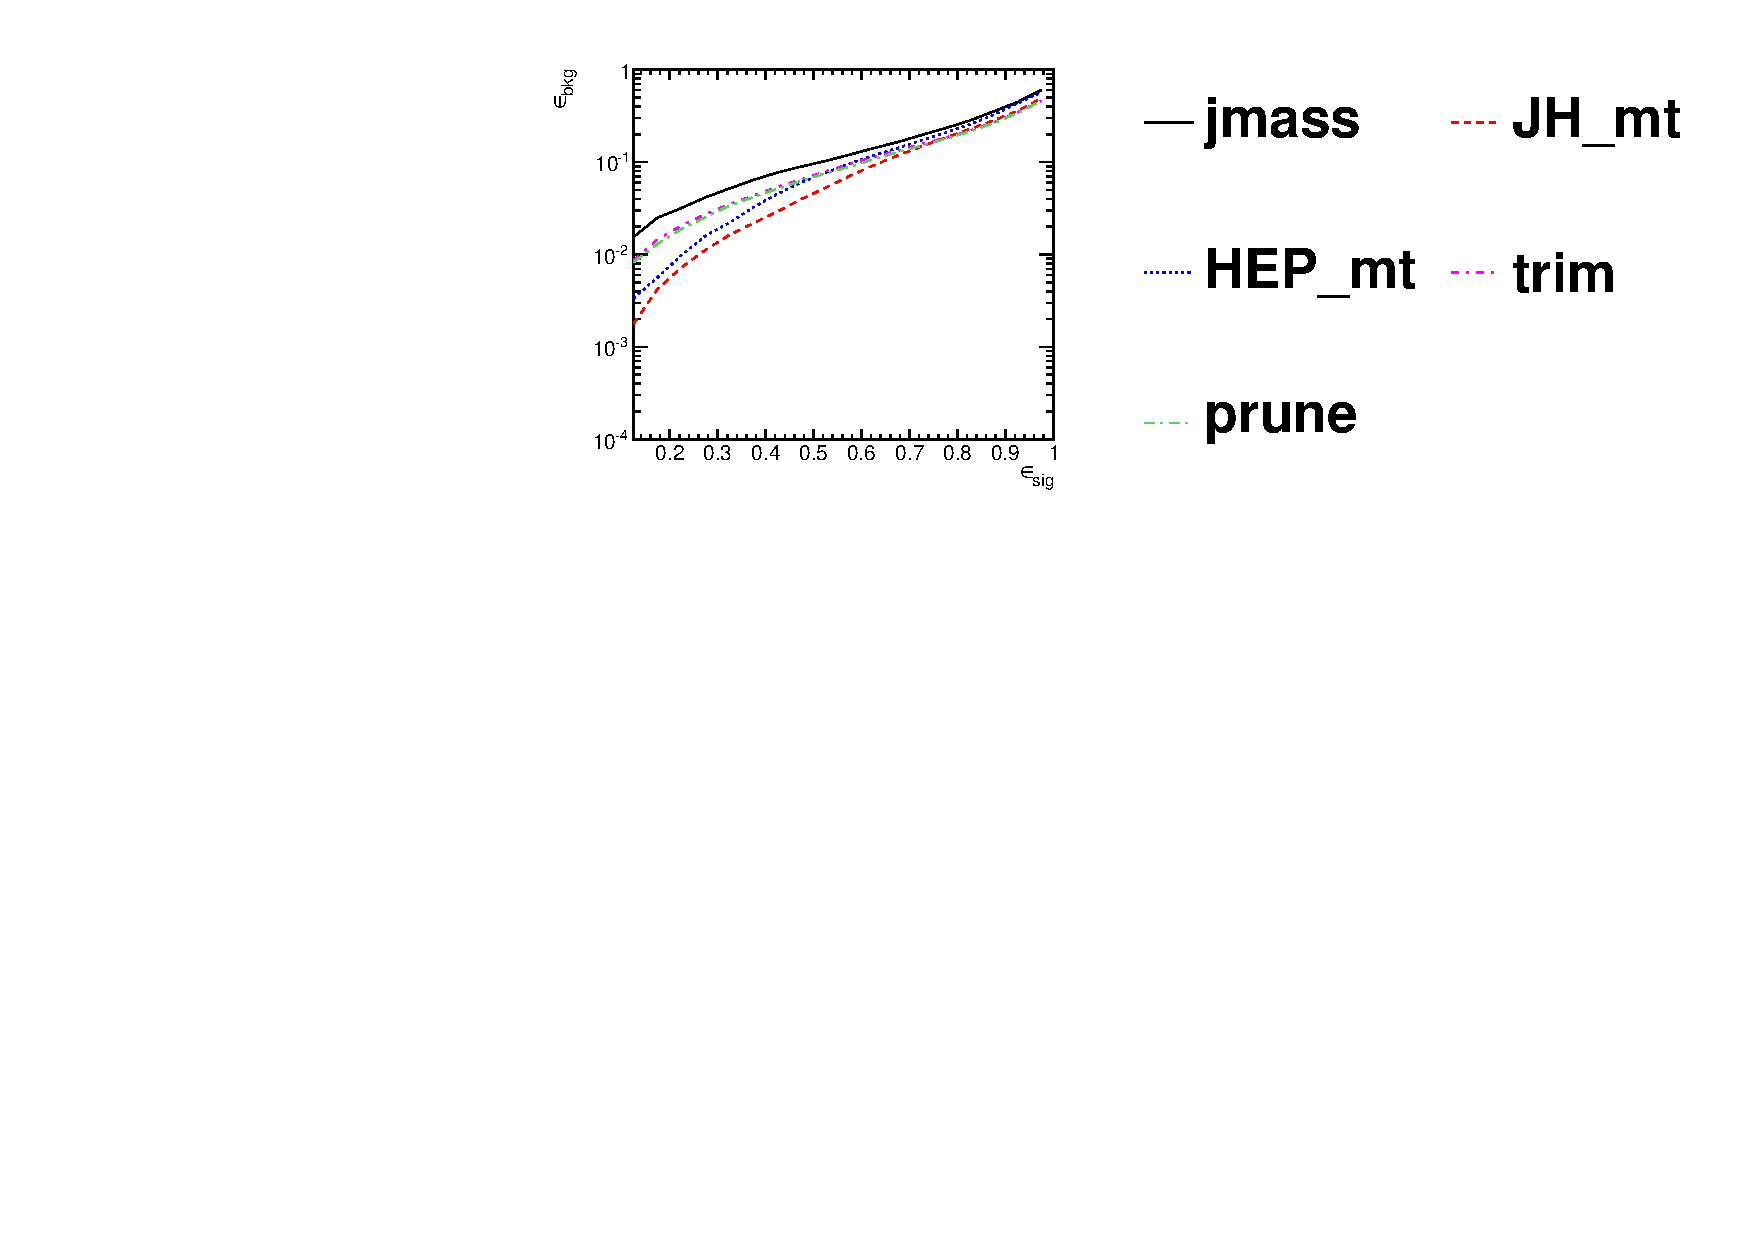
\includegraphics[width=0.49\textwidth]{./Figures/TTagging/single_variable/pT.1TeV.R.0.8/Rocs_top_mass.pdf}\label{fig:single_variable_ROC_topmass}}
\caption{Comparison of single-variable top-tagging performance in the $\pt= 1-1.1$ GeV bin using the anti-\kT, R=0.8 algorithm.}
\label{fig:single_variable_ROC}
\end{figure*}

Of the two top-tagging algorithms, it is apparent from Figure~\ref{fig:single_variable_ROC} that the Johns Hopkins tagger out-performs the HEPTopTagger in terms of its background rejection at fixed signal efficiency for both the top and $W$ candidate masses; this is expected, as the HEPTopTagger was designed to reconstruct moderate-\pt top jets in $ttH$ events (for a proposed high-\pt variant of the HEPTopTagger, see \cite{Schaetzel:2013vka}). In Figure~\ref{fig:topmass_histogram_HEP_JH}, we show the histograms for the top mass output from the JH and HEPTopTagger for different $R$ in the \pt =  1.5-1.6 TeV bin, and in Figure~\ref{fig:topmass_histogram_HEP_JH_pT} for different \pt at $R=0.8$, optimized at a signal efficiency of 30\%. 
A particular feature of the HepTopTagger algorithm is that, after the jet is filtered to select the five hardest subjets, the three subjets are chosen which most closely reconstruct the top mass. This requirement tends to shape a peak in the QCD background around $m_t$ for the HEPTopTagger, as can be seen from Figures~\ref{fig:topmass_histogram_HEP_R12} and~\ref{fig:topmass_histogram_HEP_pT15}; this is the likely reason for the better performance of the JH tagger, which has no such requirement.
It has been suggested  \cite{Anders:2013oga} that performance in the HEPTopTagger may be improved by selecting the three subjets reconstructing the top only among those that pass the $W$ mass constraints, which somewhat reduces the shaping of the background. The discrepancy between the JH and the 
HEPTopTagger is more pronounced  at higher $\pt$ and larger jet radius (see Figures~\ref{fig:ptcomparison_singletopmass_top} and \ref{fig:Rcomparison_singletopmass_top}). 

\begin{figure*}
\centering
\subfigure[JH, $R=0.4$]{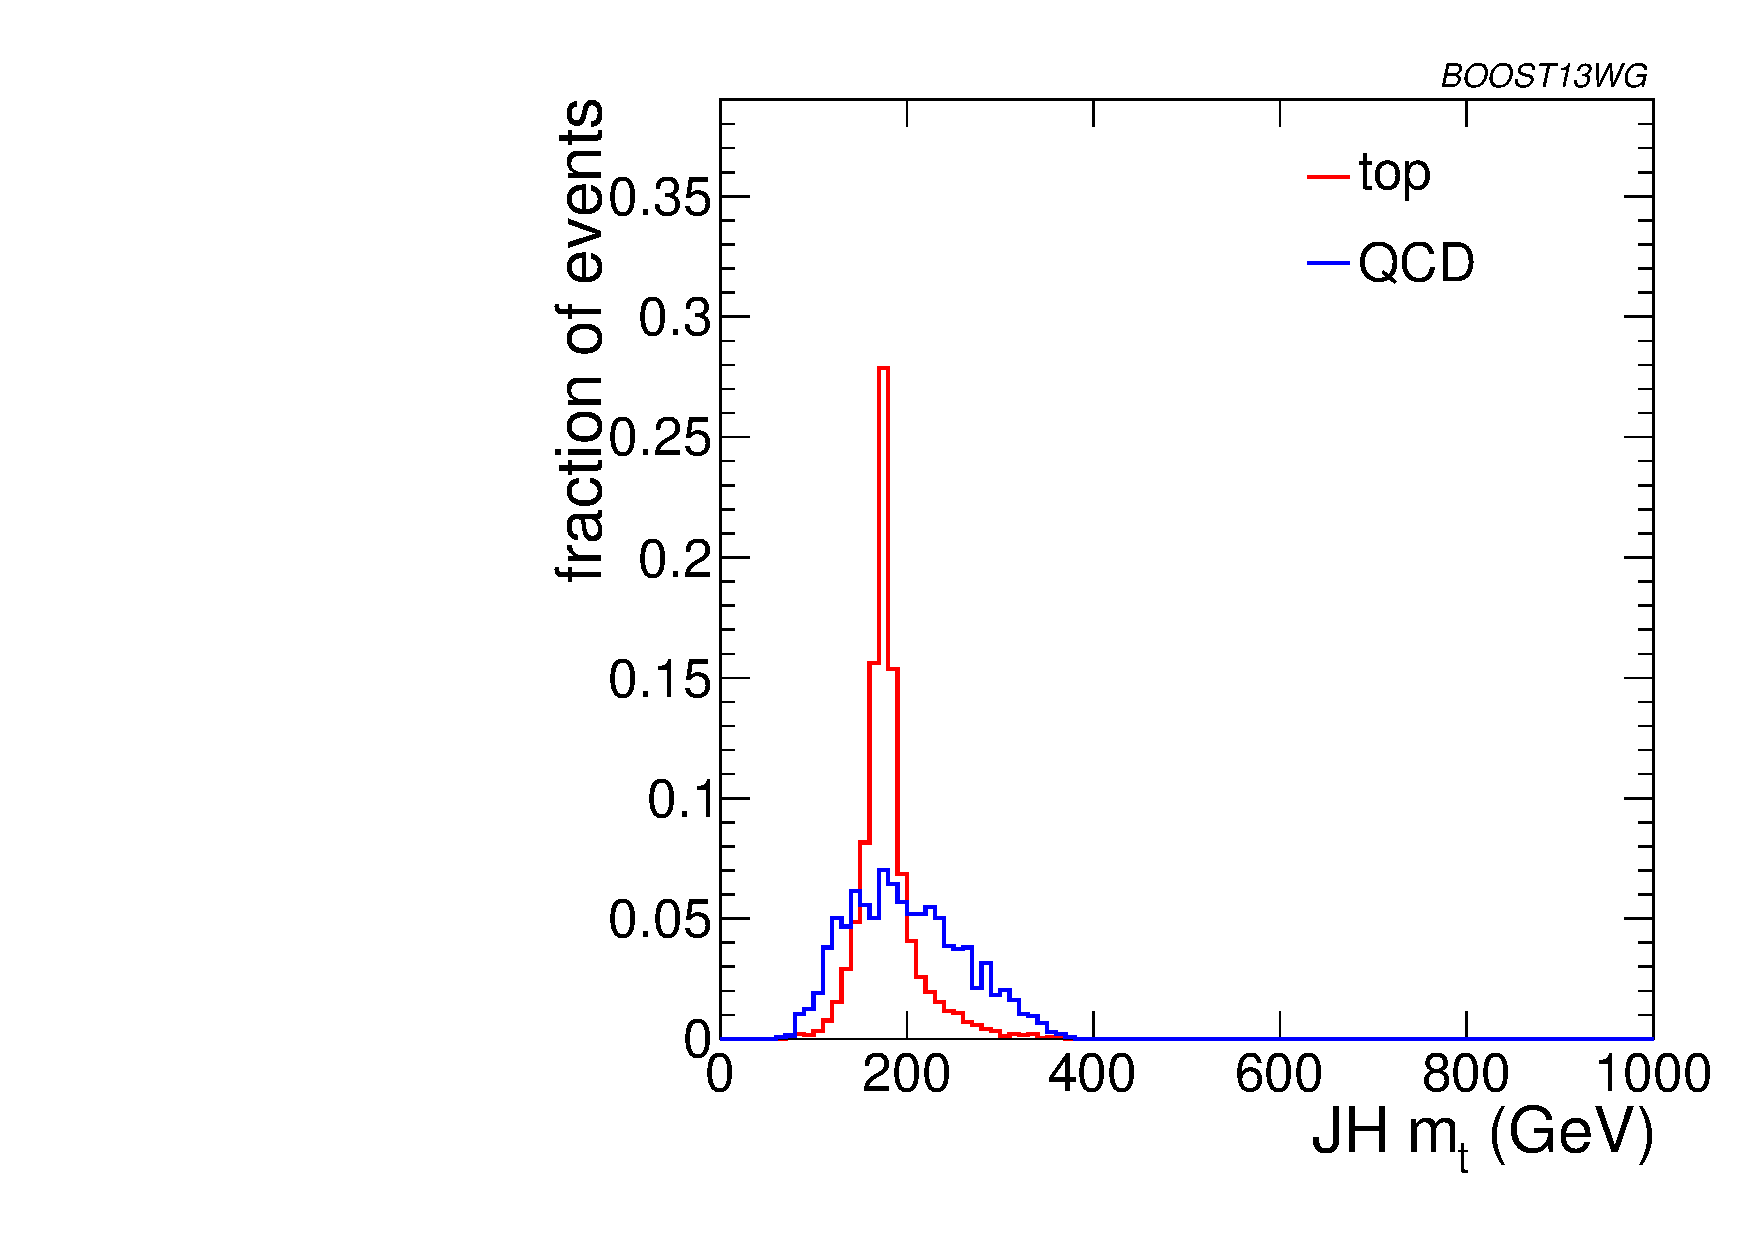
\includegraphics[width=0.245\textwidth]{./Figures/TTagging/single_variable/pT.1.5TeV.R.0.4/h_JH_mt_opt_mt.pdf}}
\subfigure[HEP, $R=0.4$]{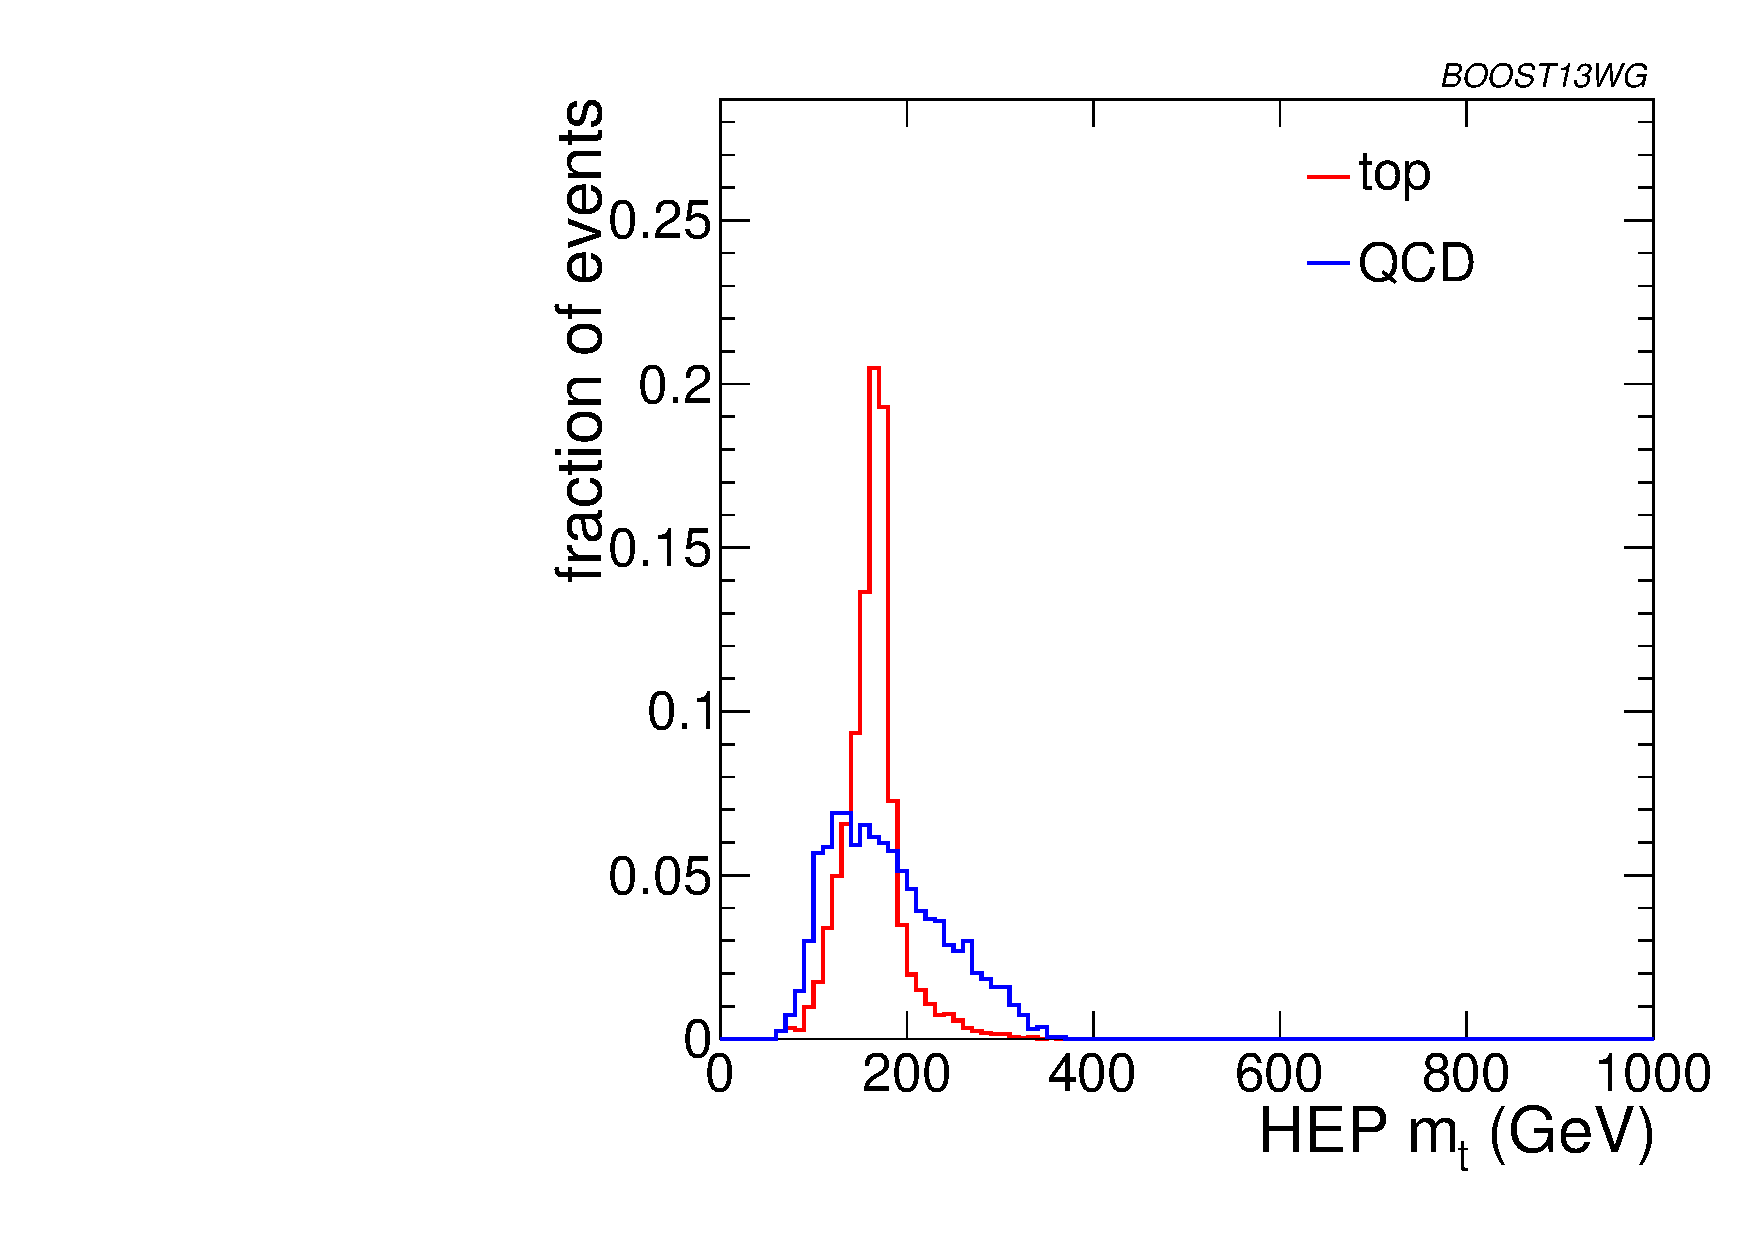
\includegraphics[width=0.245\textwidth]{./Figures/TTagging/single_variable/pT.1.5TeV.R.0.4/h_HEP_mt_opt_mt.pdf}}
\subfigure[JH, $R=1.2$]{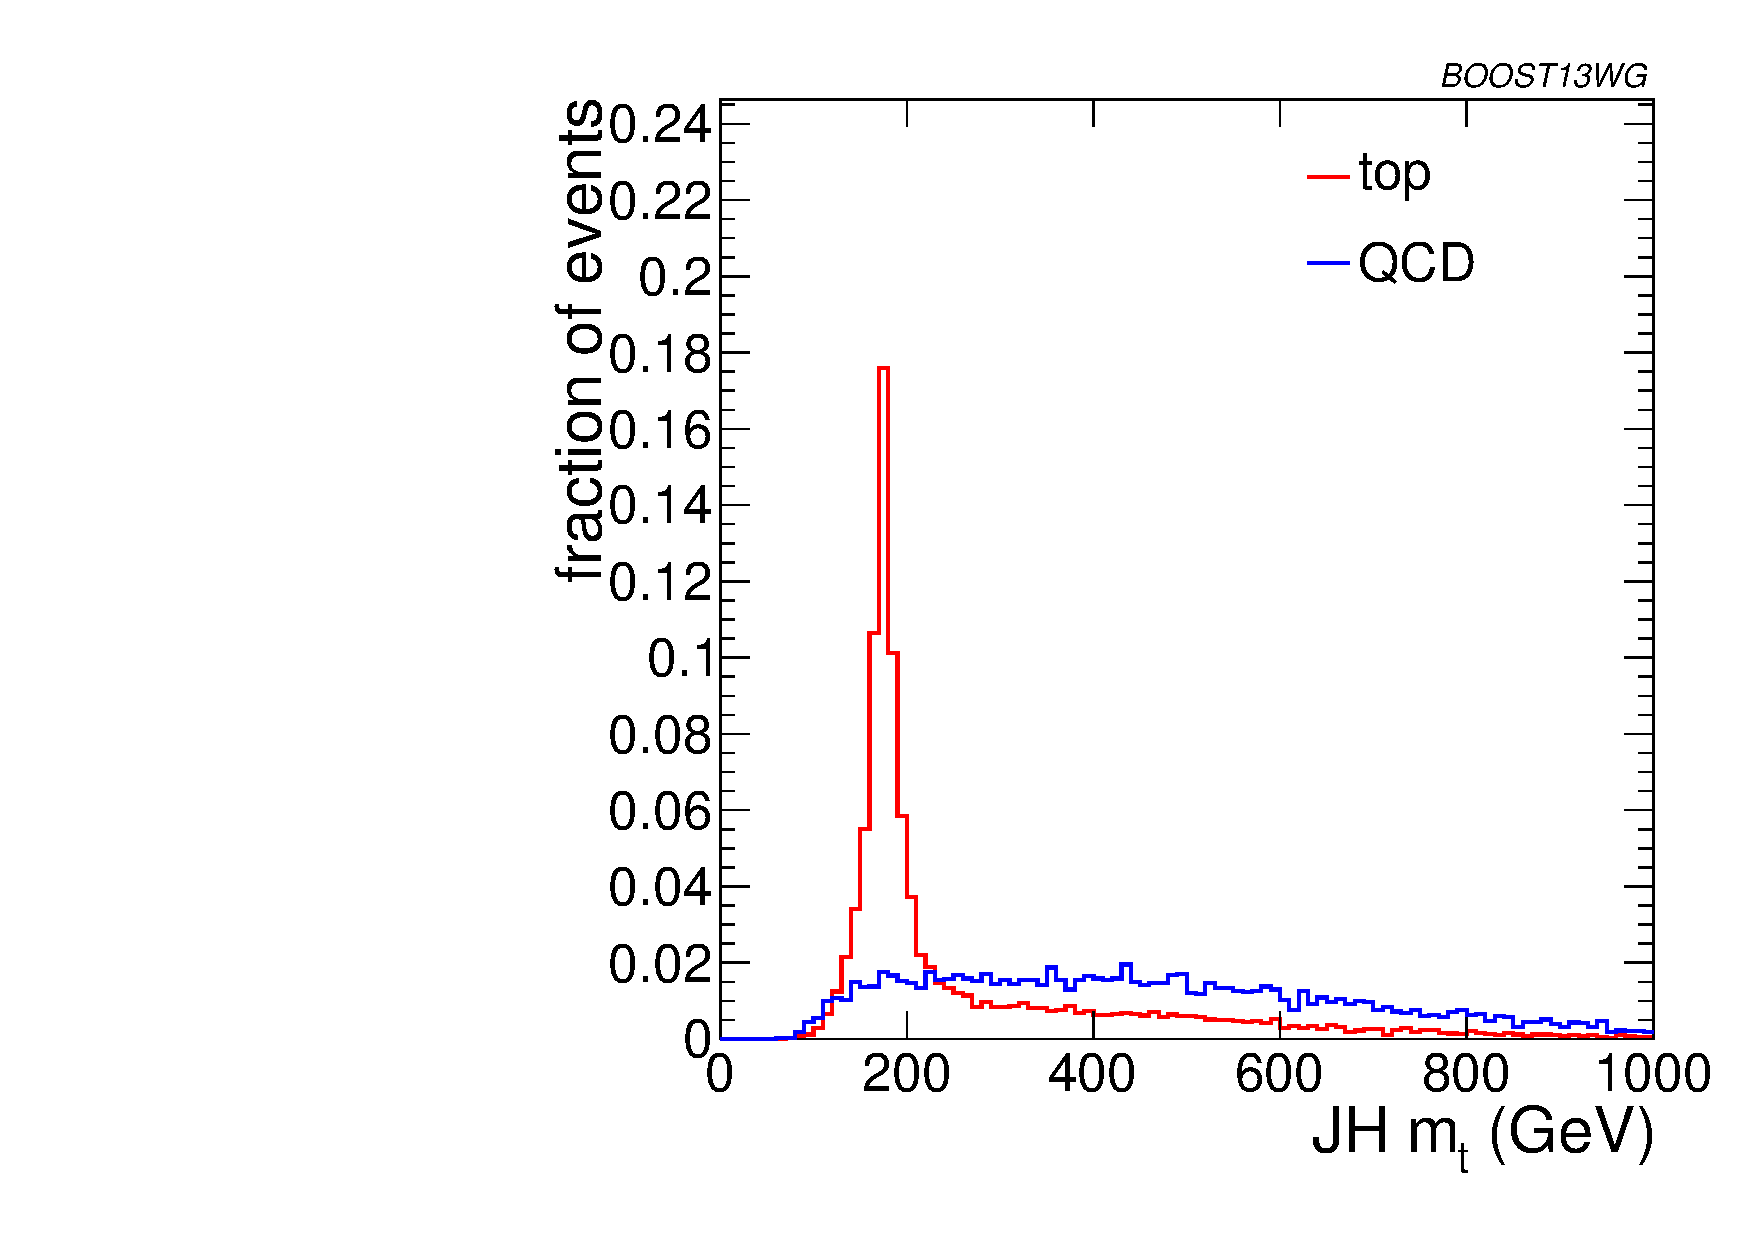
\includegraphics[width=0.245\textwidth]{./Figures/TTagging/single_variable/pT.1.5TeV.R.1.2/h_JH_mt_opt_mt.pdf}}
\subfigure[HEP, $R=1.2$]{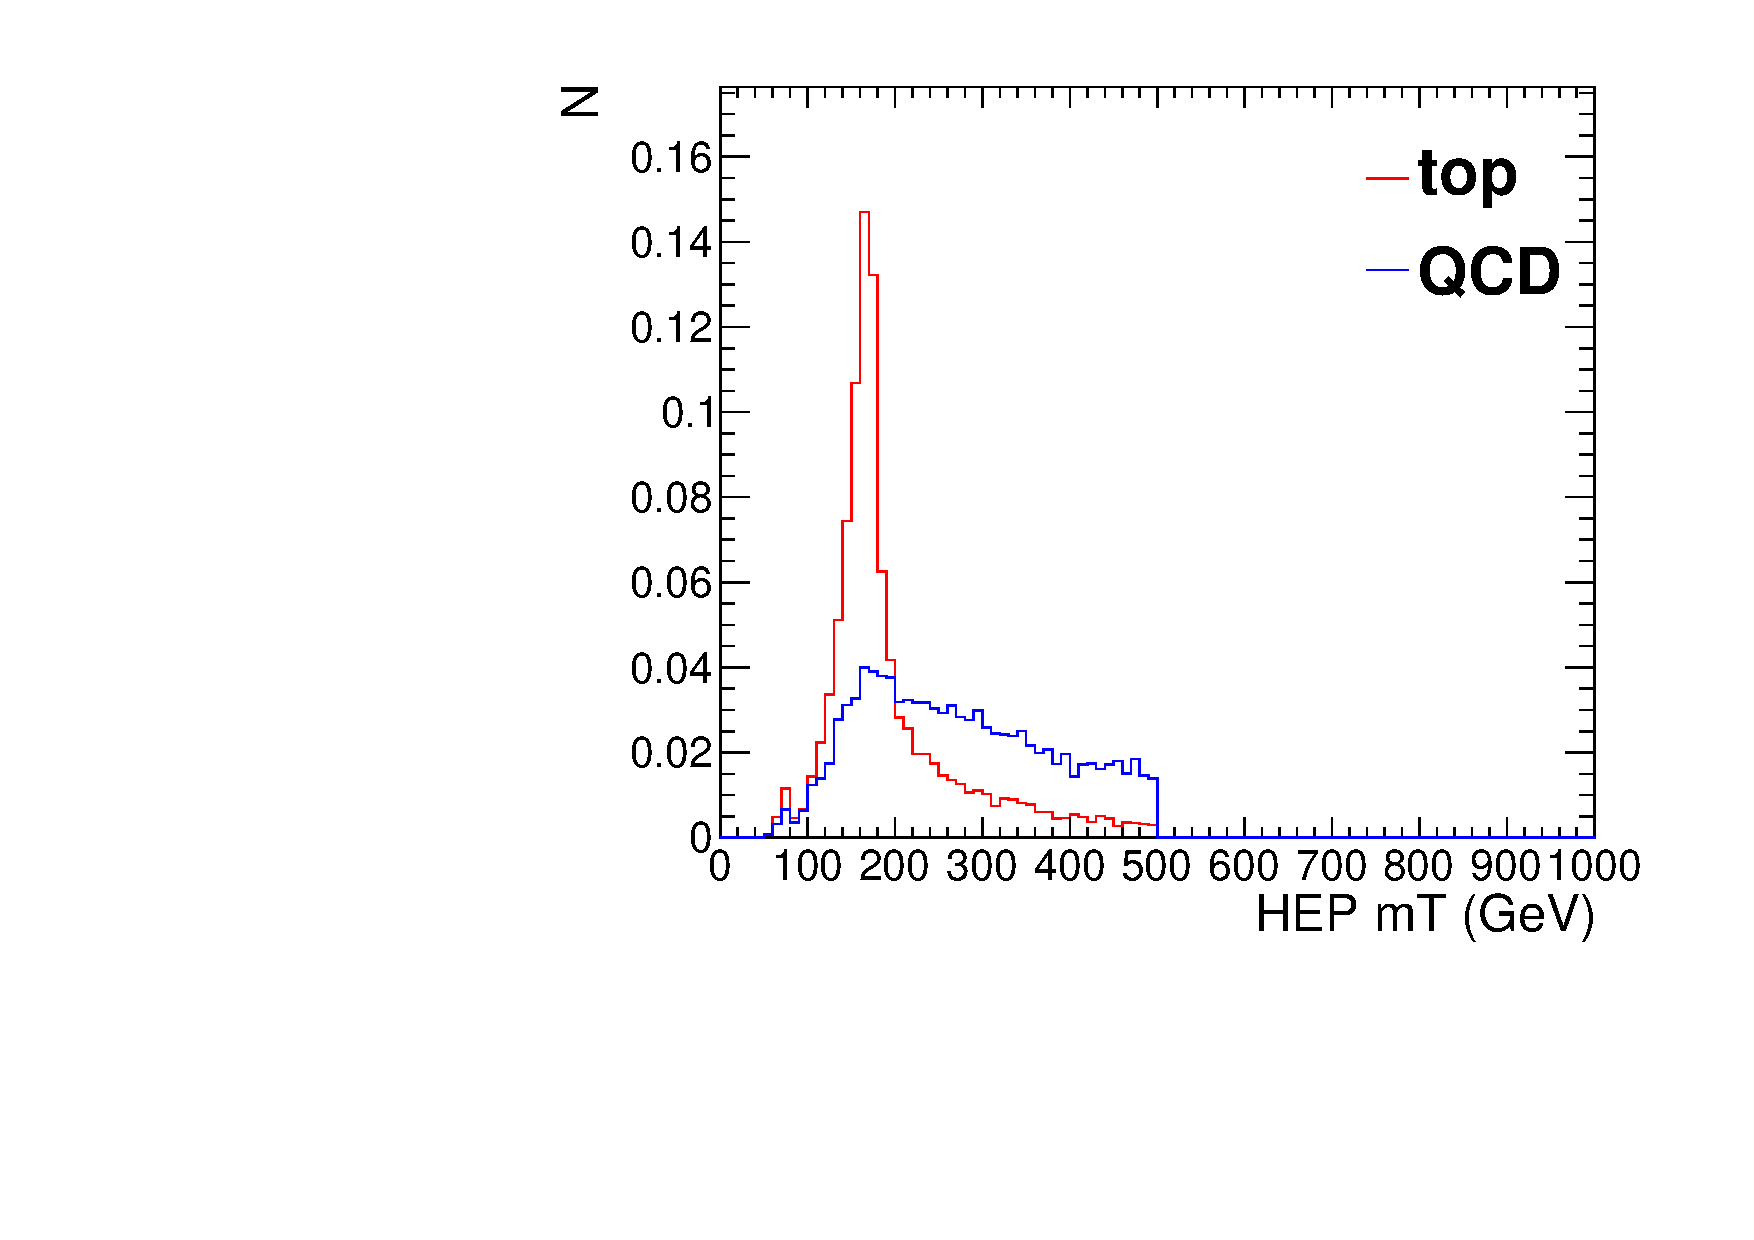
\includegraphics[width=0.245\textwidth]{./Figures/TTagging/single_variable/pT.1.5TeV.R.1.2/h_HEP_mt_opt_mt.pdf}\label{fig:topmass_histogram_HEP_R12}}\\
\subfigure[prune, $R=0.4$]{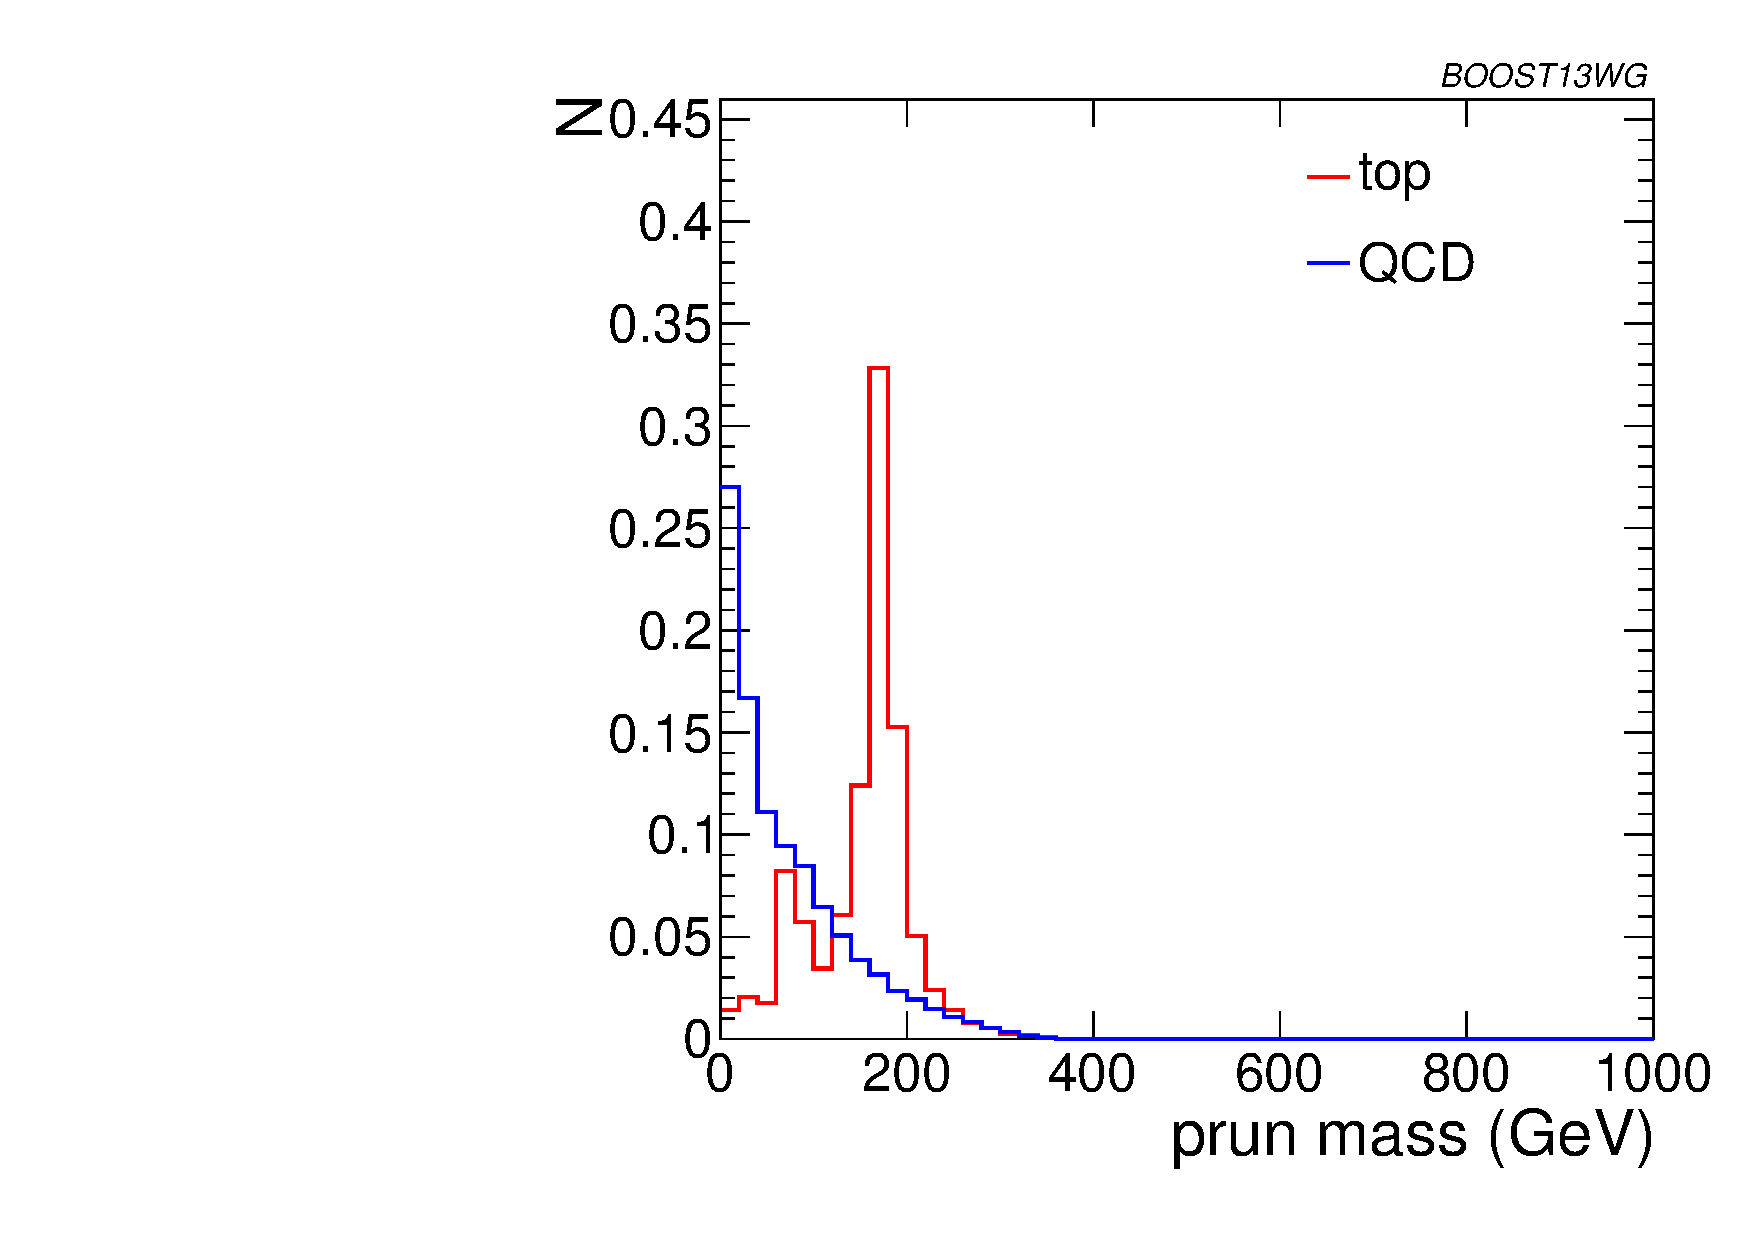
\includegraphics[width=0.245\textwidth]{./Figures/TTagging/single_variable/pT.1.5TeV.R.0.4/h_prun_R_0_4.pdf}}
\subfigure[trim, $R=0.4$]{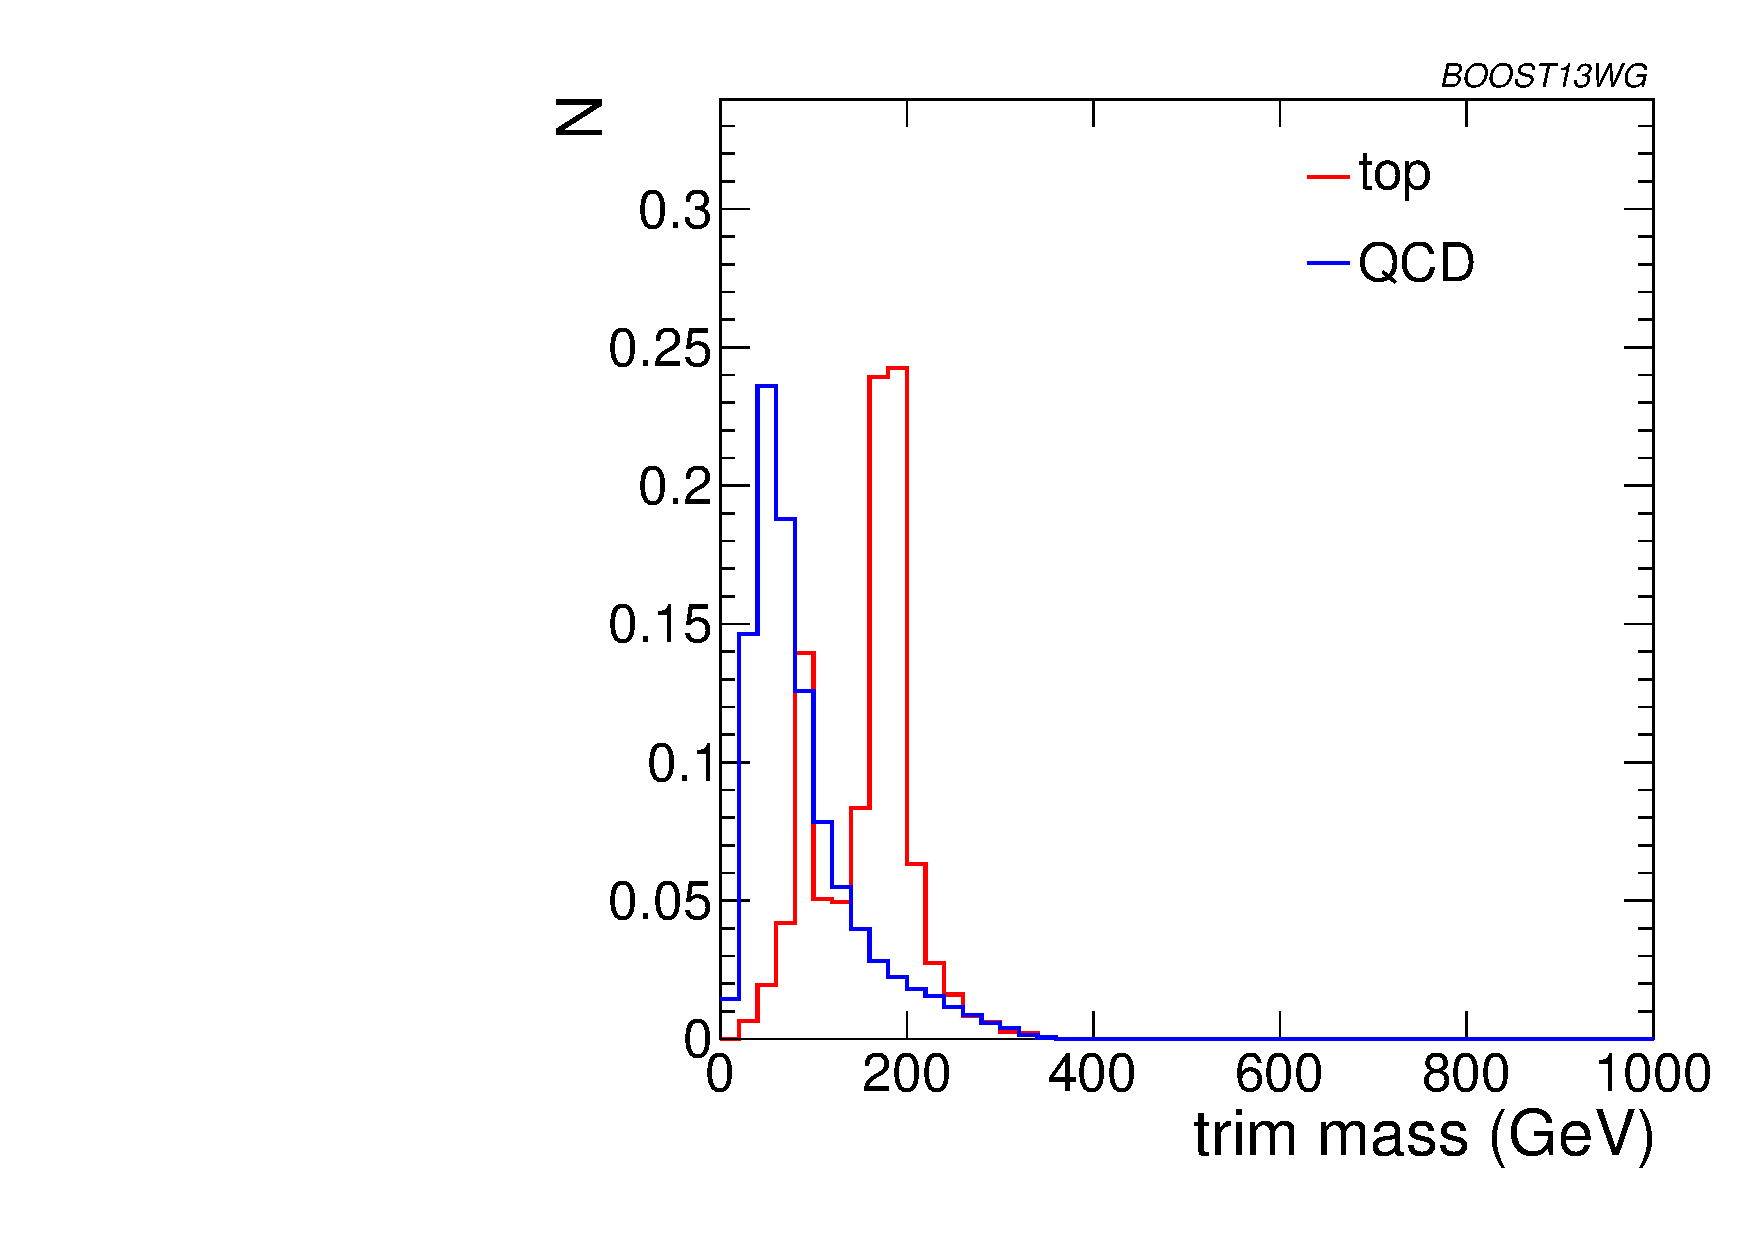
\includegraphics[width=0.245\textwidth]{./Figures/TTagging/single_variable/pT.1.5TeV.R.0.4/h_trim_R_0_4.pdf}}
\subfigure[prune, $R=1.2$]{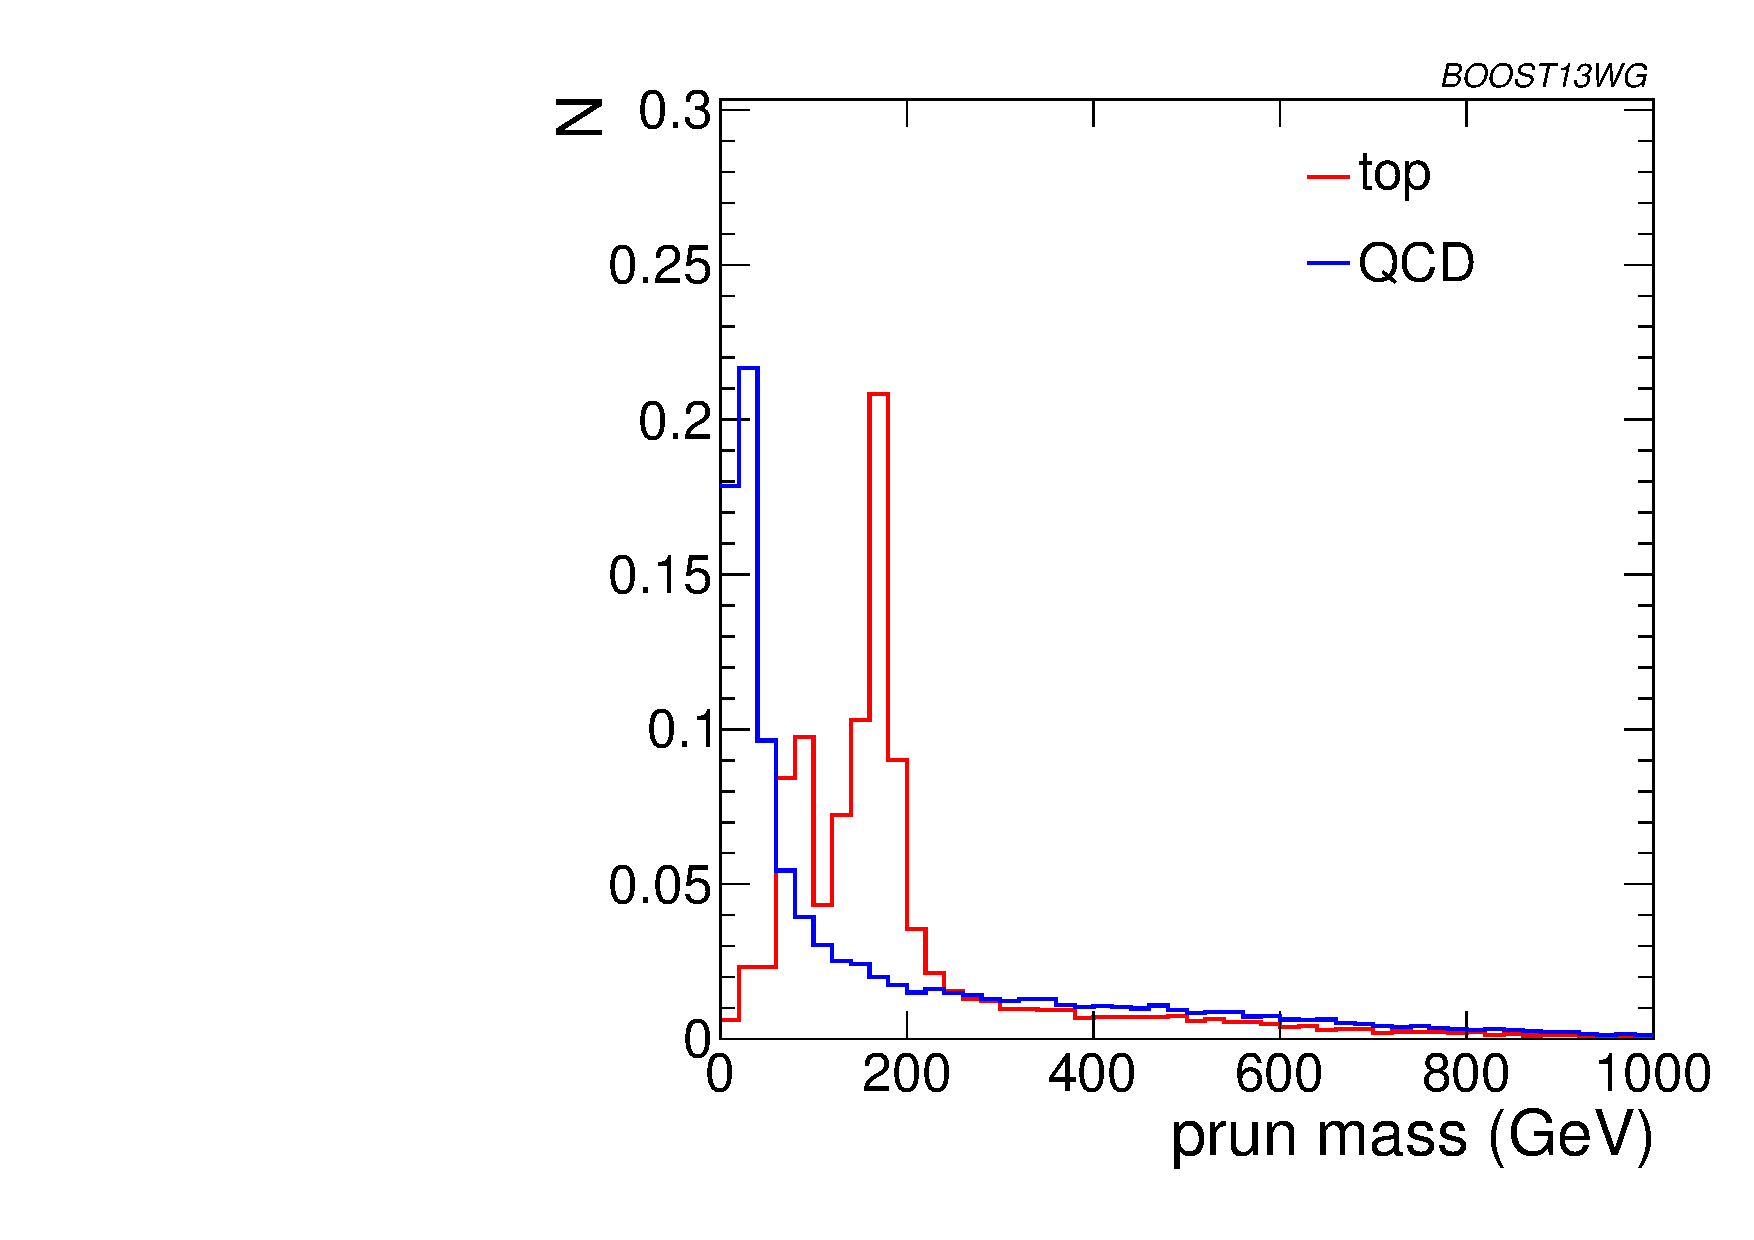
\includegraphics[width=0.245\textwidth]{./Figures/TTagging/single_variable/pT.1.5TeV.R.1.2/h_prun_R_1_2.pdf}}
\subfigure[trim, $R=1.2$]{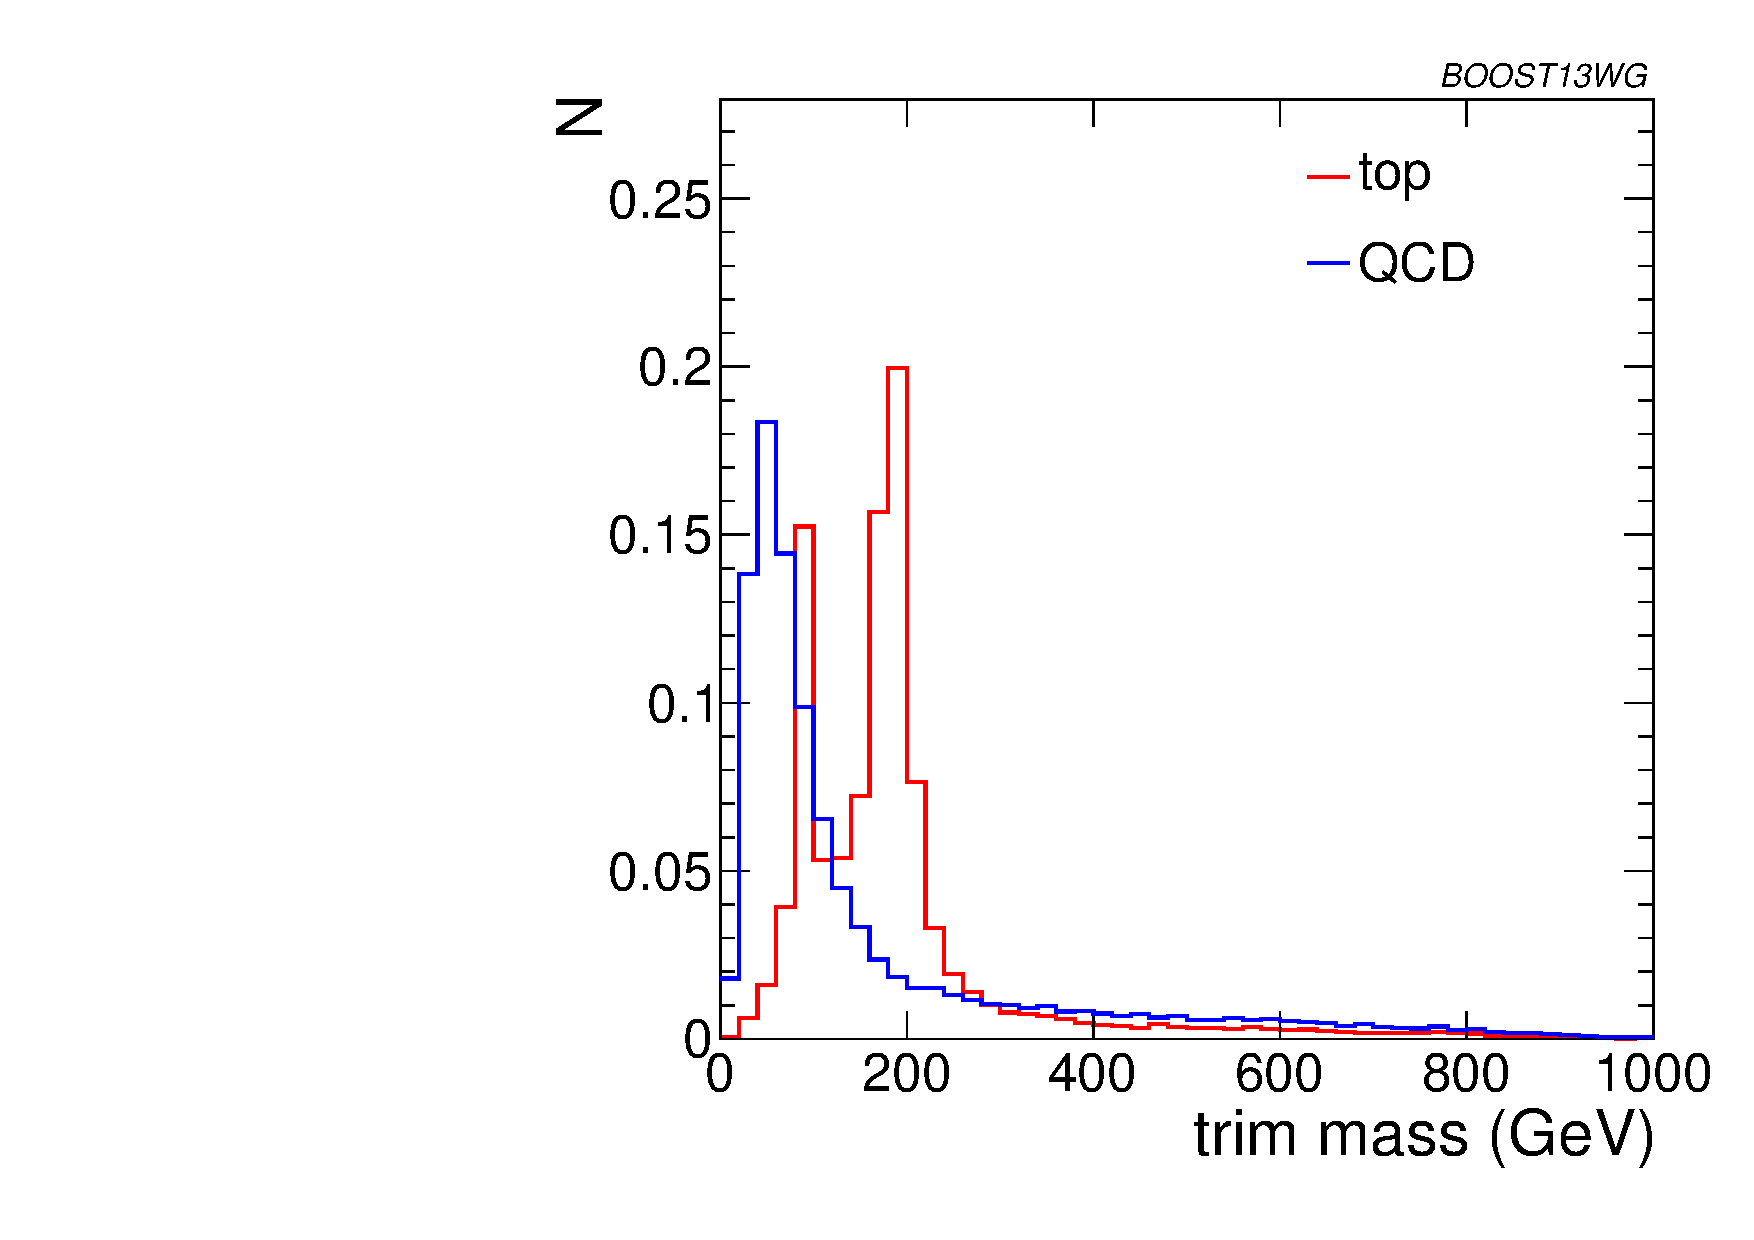
\includegraphics[width=0.245\textwidth]{./Figures/TTagging/single_variable/pT.1.5TeV.R.1.2/h_trim_R_1_2.pdf}}
\caption{Comparison of top mass reconstruction with the Johns Hopkins (JH), HEPTopTaggers (HEP), pruning, and trimming at different $R$ using the \antikt algorithm in the \pt = 1.5-1.6 \TeV bin. Each histogram is shown for the working point optimized for best performance with $m_t$ in the $0.3$-$0.35$ signal efficiency bin, and is normalized to the fraction of events passing the tagger. In this and subsequent plots, the HEPTopTagger distribution cuts off at 500 \GeV because the tagger fails to tag jets with a larger mass.}
\label{fig:topmass_histogram_HEP_JH}
\end{figure*}

\begin{figure*}
\centering
\subfigure[JH, \pt = 600-700 \GeV]{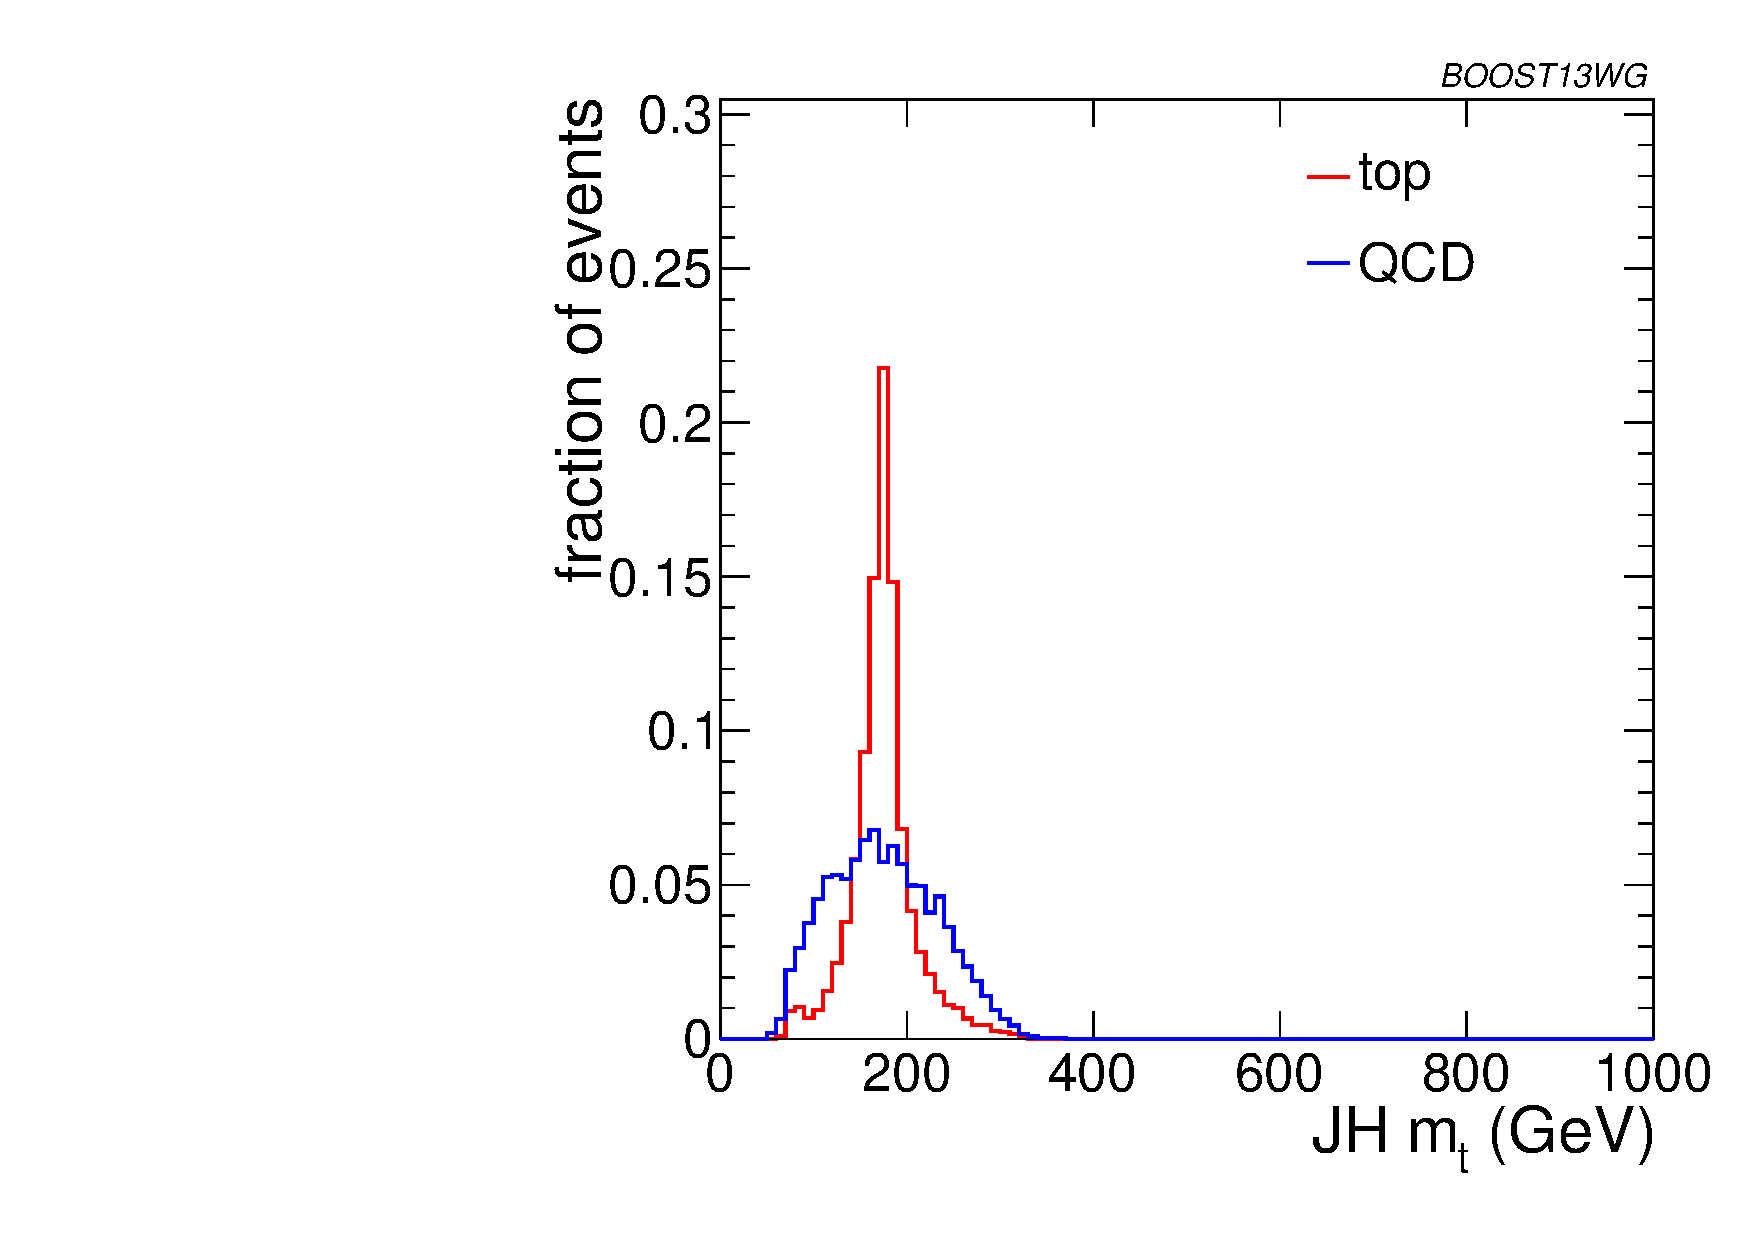
\includegraphics[width=0.245\textwidth]{./Figures/TTagging/single_variable/pT.600GeV.R.0.8/h_JH_mt_pT_0_6.pdf}}
\subfigure[HEP, \pt = 600-700 \GeV]{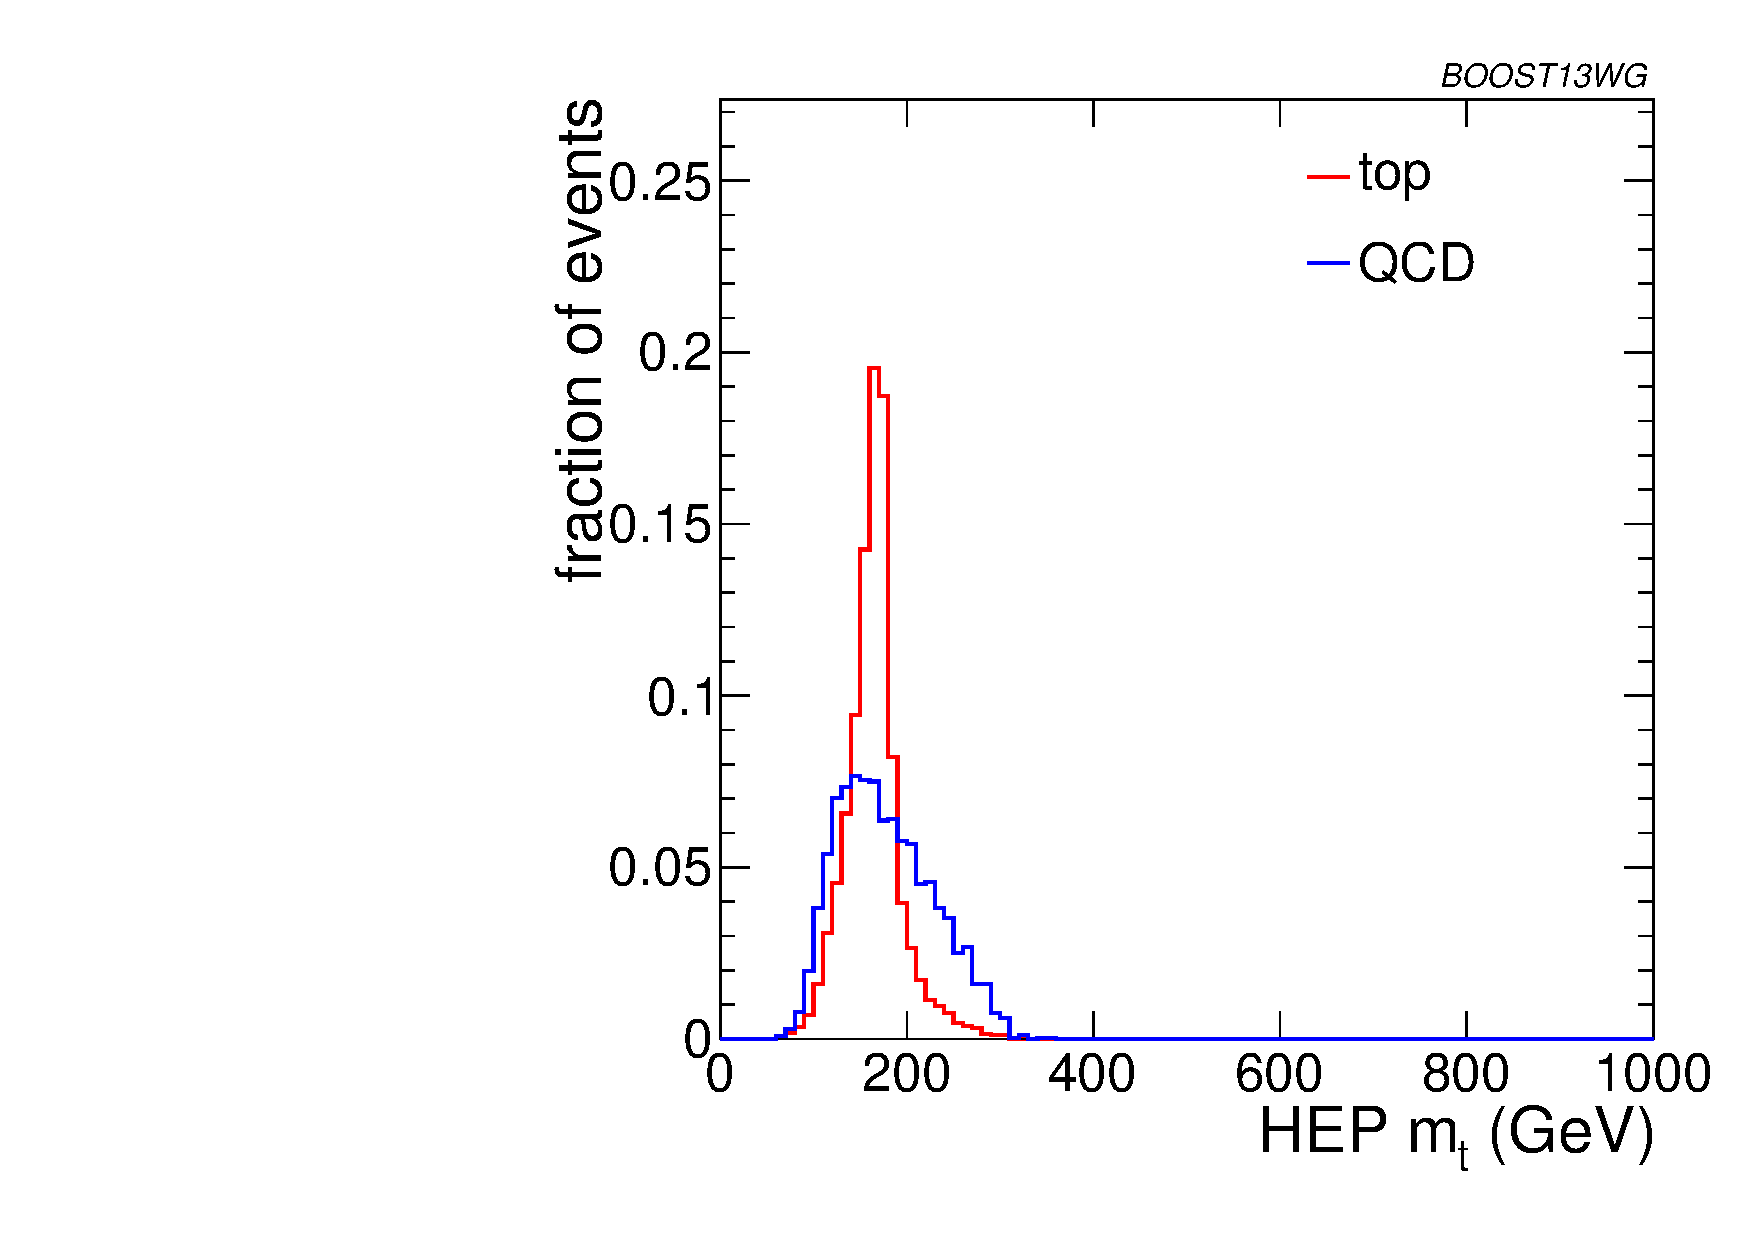
\includegraphics[width=0.245\textwidth]{./Figures/TTagging/single_variable/pT.600GeV.R.0.8/h_HEP_mt_pT_0_6.pdf}}
\subfigure[JH, \pt = 1.5-1.6 \TeV]{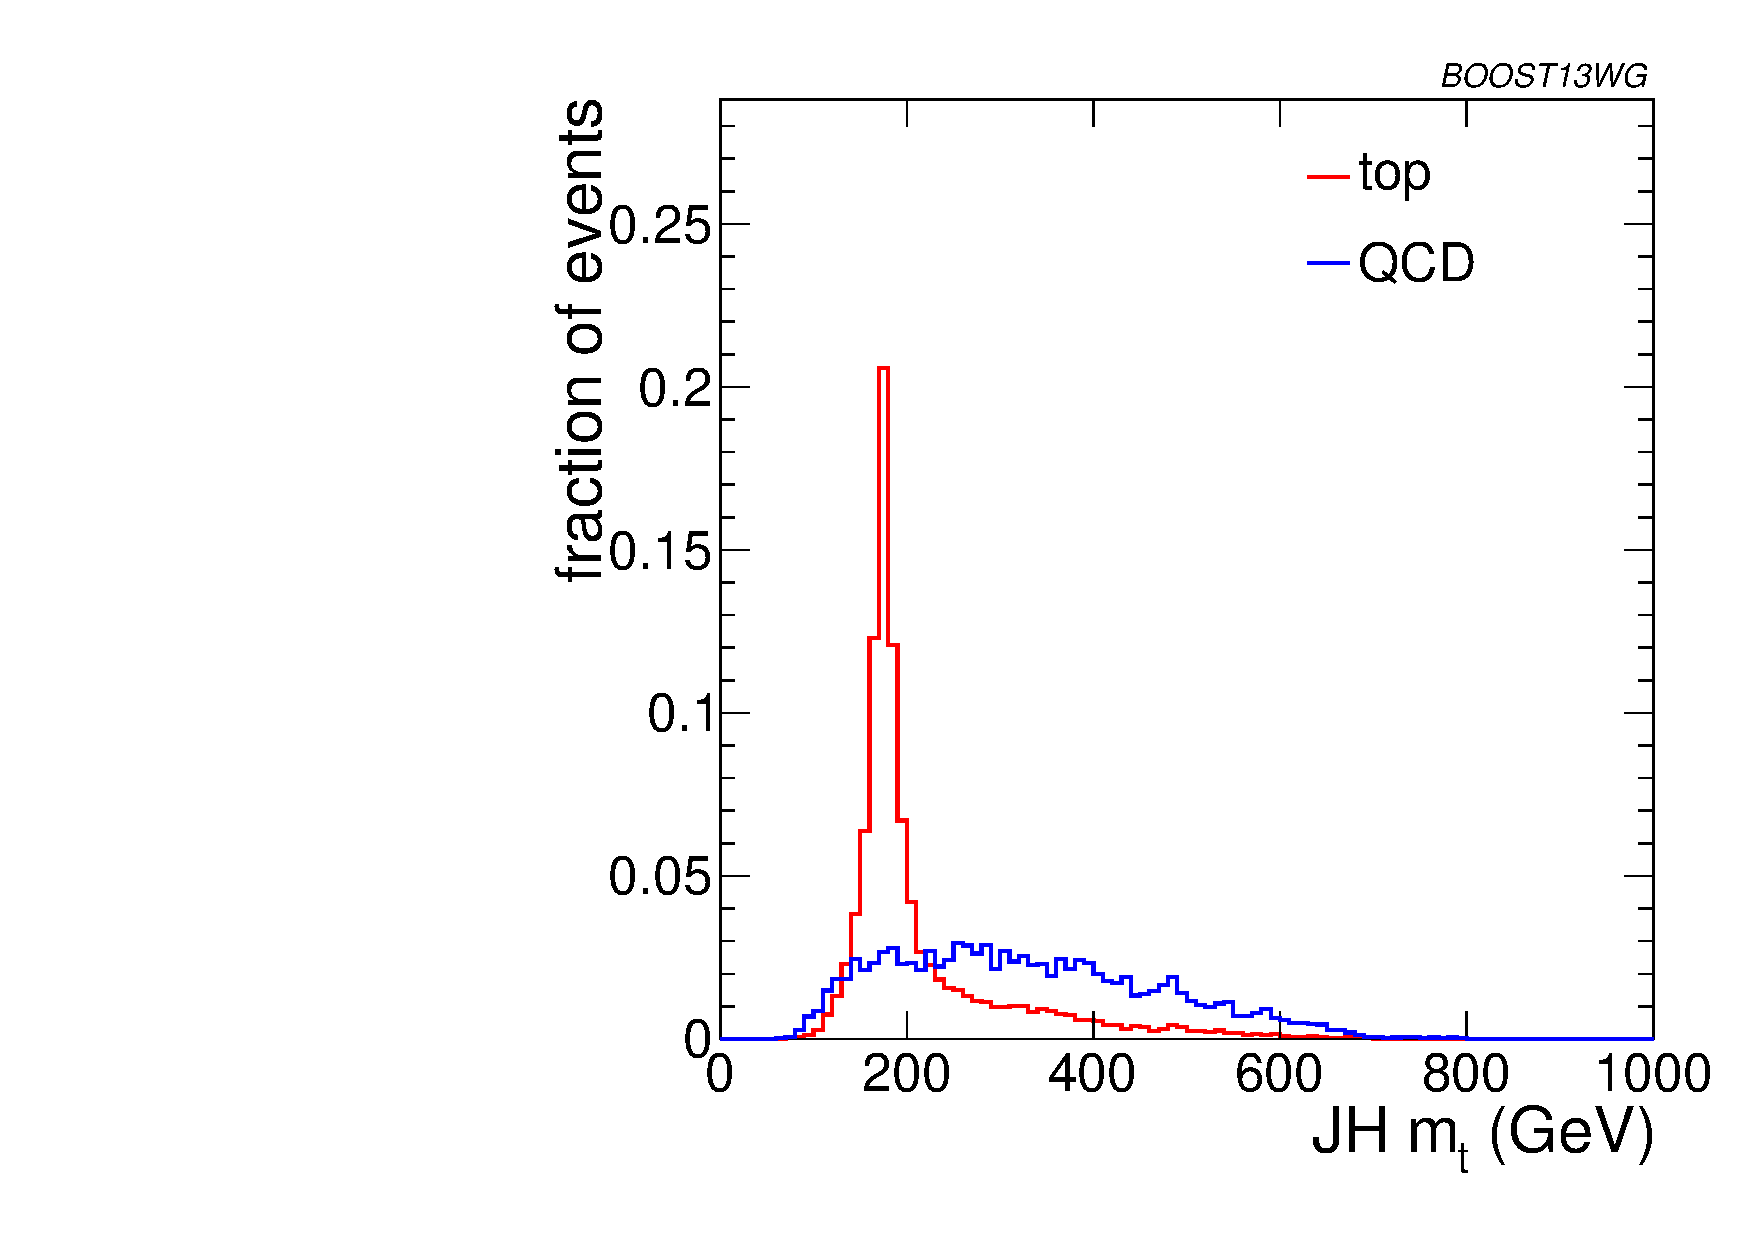
\includegraphics[width=0.245\textwidth]{./Figures/TTagging/single_variable/pT.1.5TeV.R.0.8/h_JH_mt_pT_1_5.pdf}}
\subfigure[HEP, \pt = 1.5-1.6 \TeV]{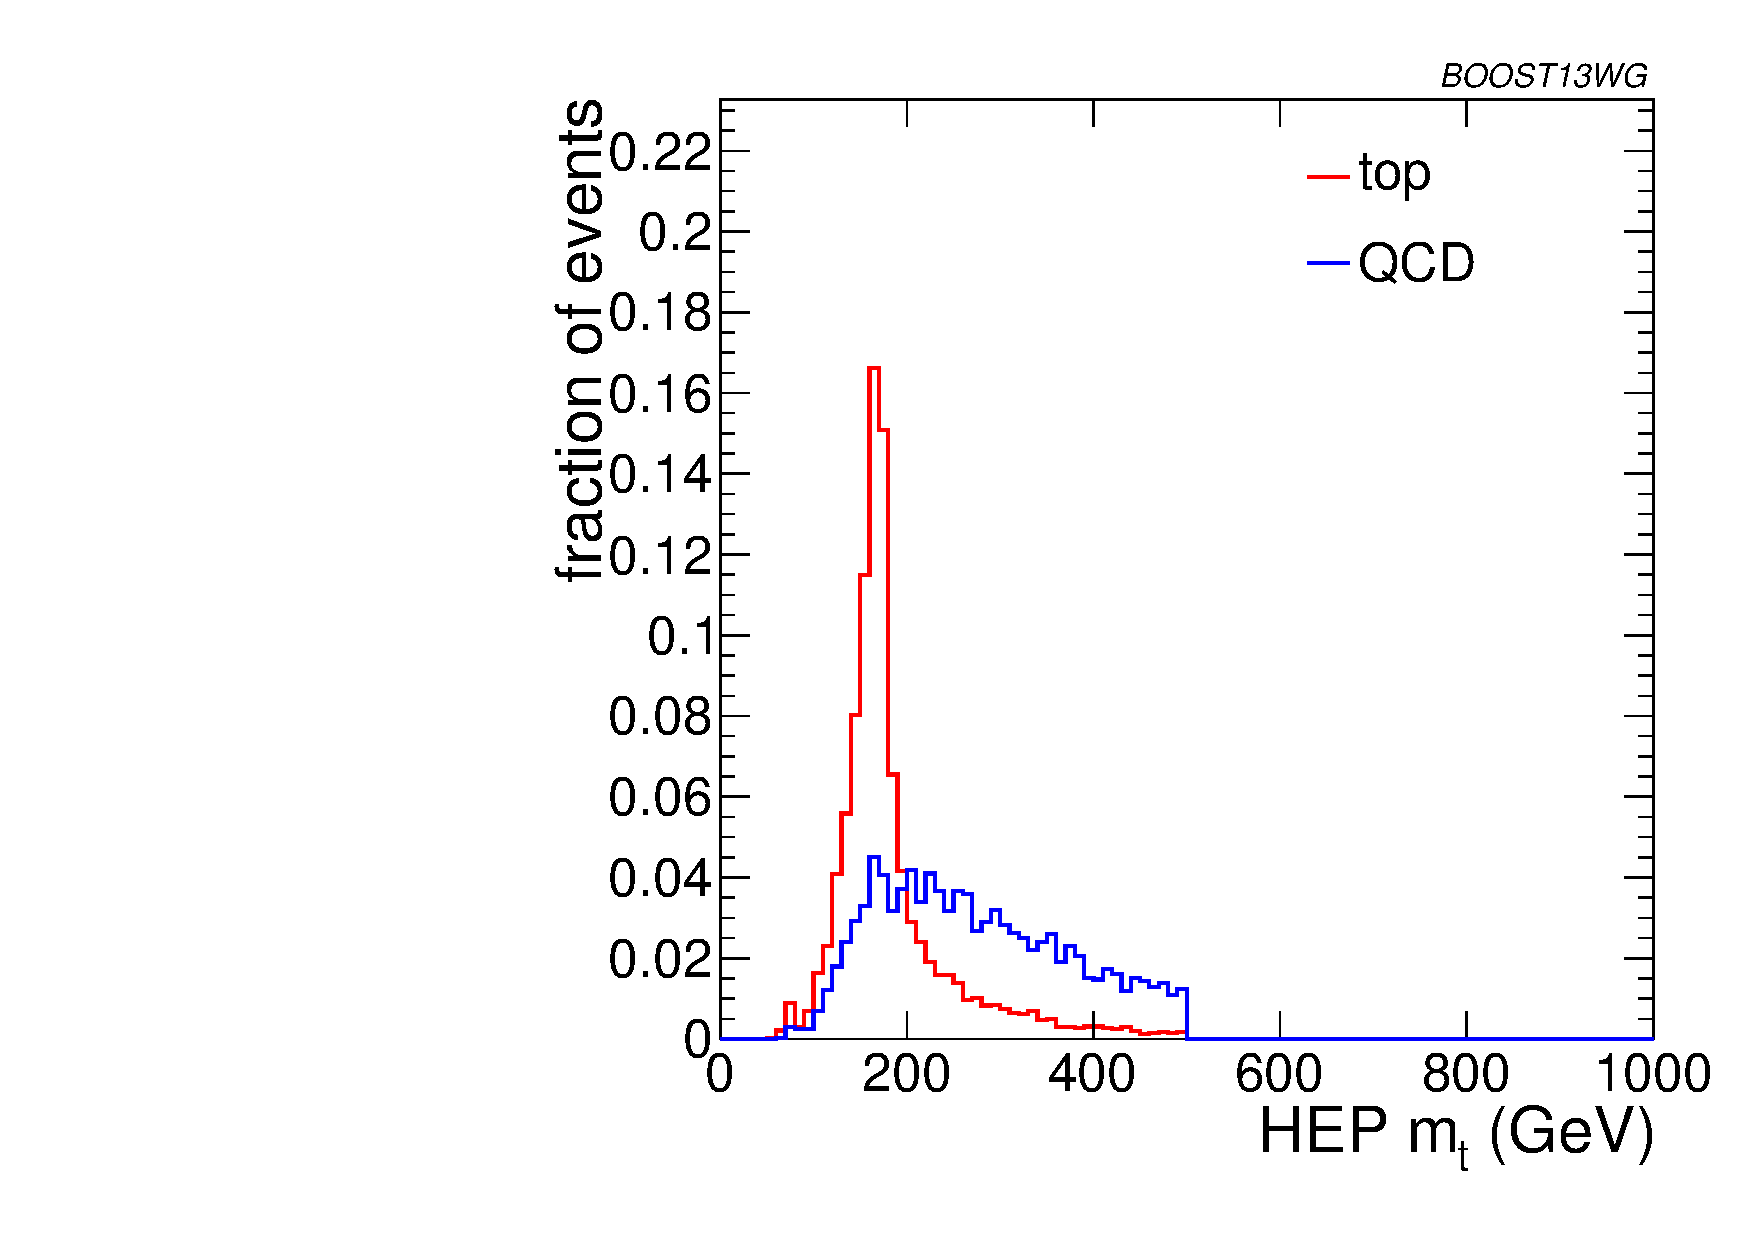
\includegraphics[width=0.245\textwidth]{./Figures/TTagging/single_variable/pT.1.5TeV.R.0.8/h_HEP_mt_pT_1_5.pdf}\label{fig:topmass_histogram_HEP_pT15}}\\
\subfigure[prune, \pt = 600-700 \GeV]{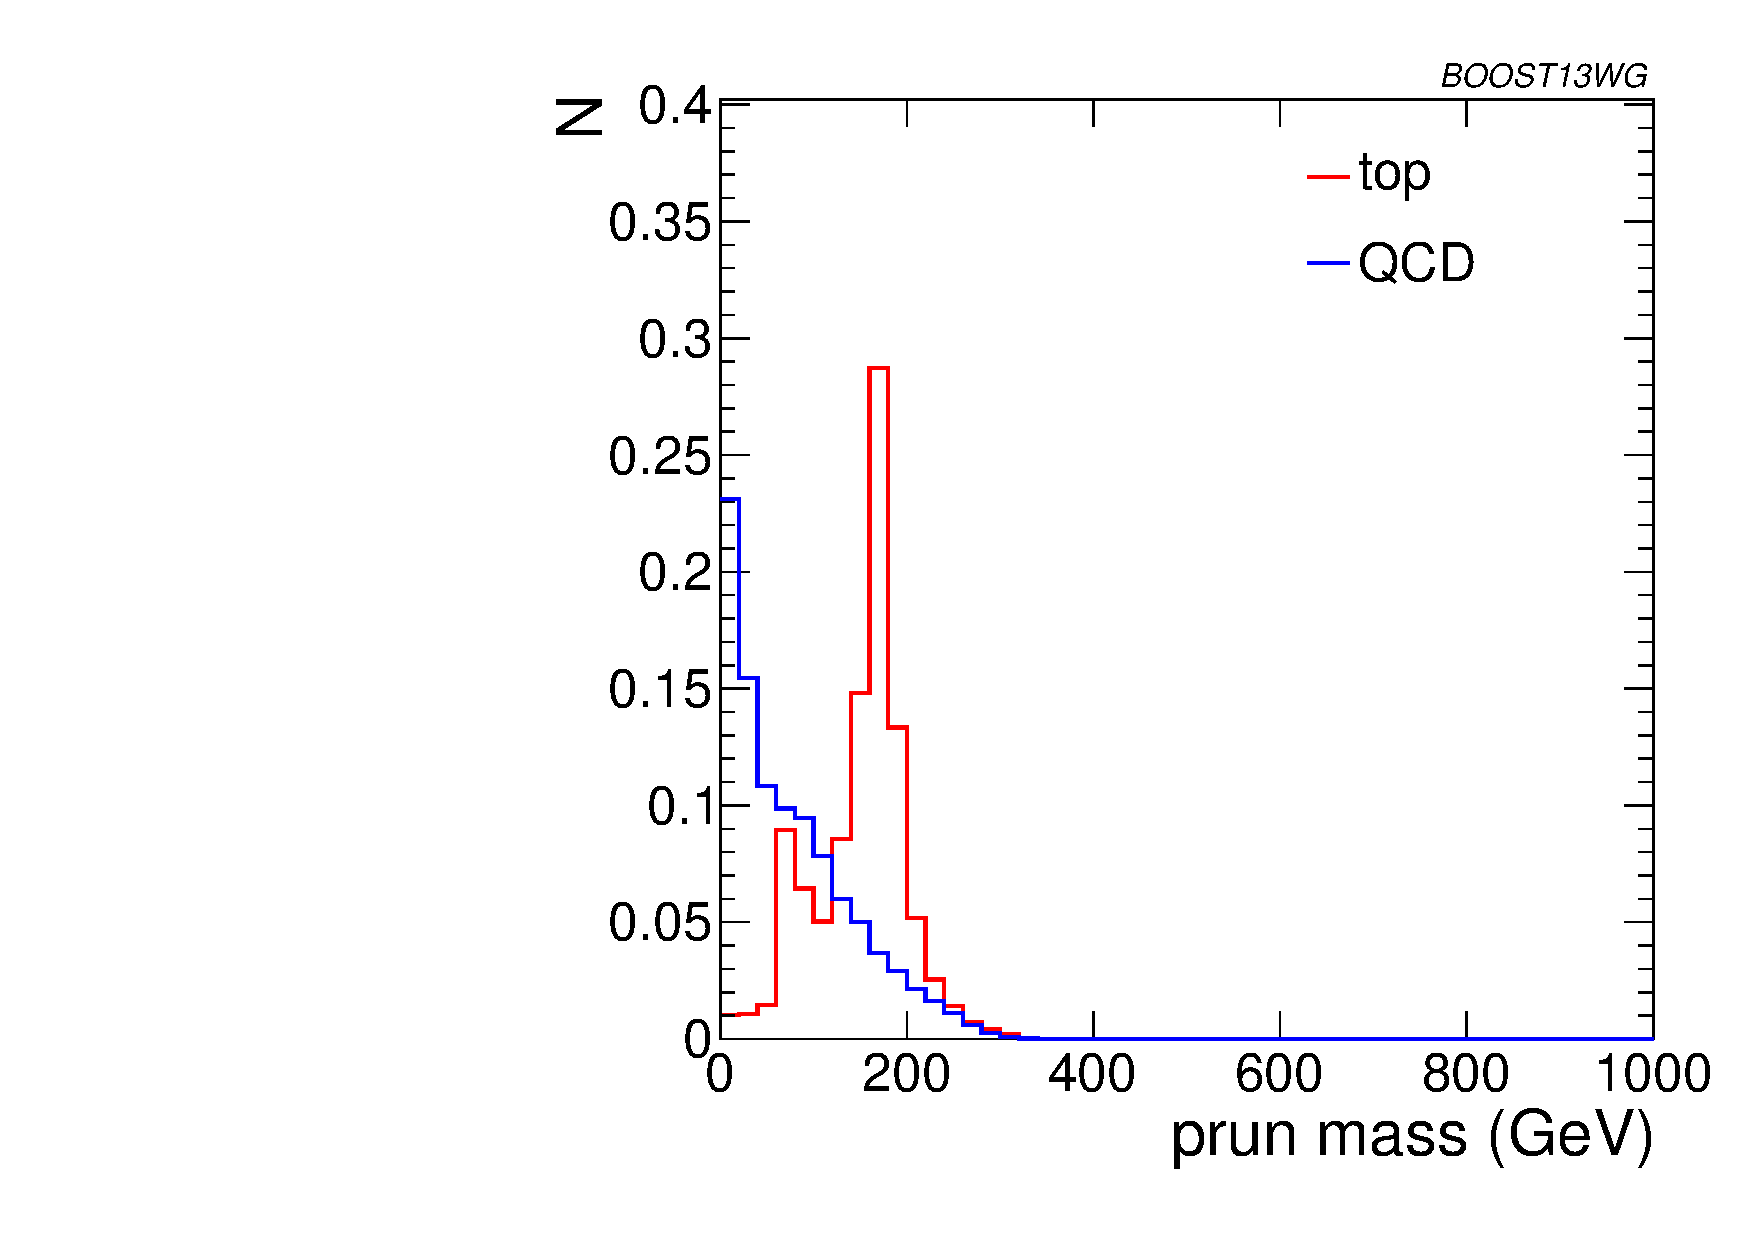
\includegraphics[width=0.245\textwidth]{./Figures/TTagging/single_variable/pT.600GeV.R.0.8/h_prun_pT_0_6.pdf}}
\subfigure[trim, \pt = 600-700 \GeV]{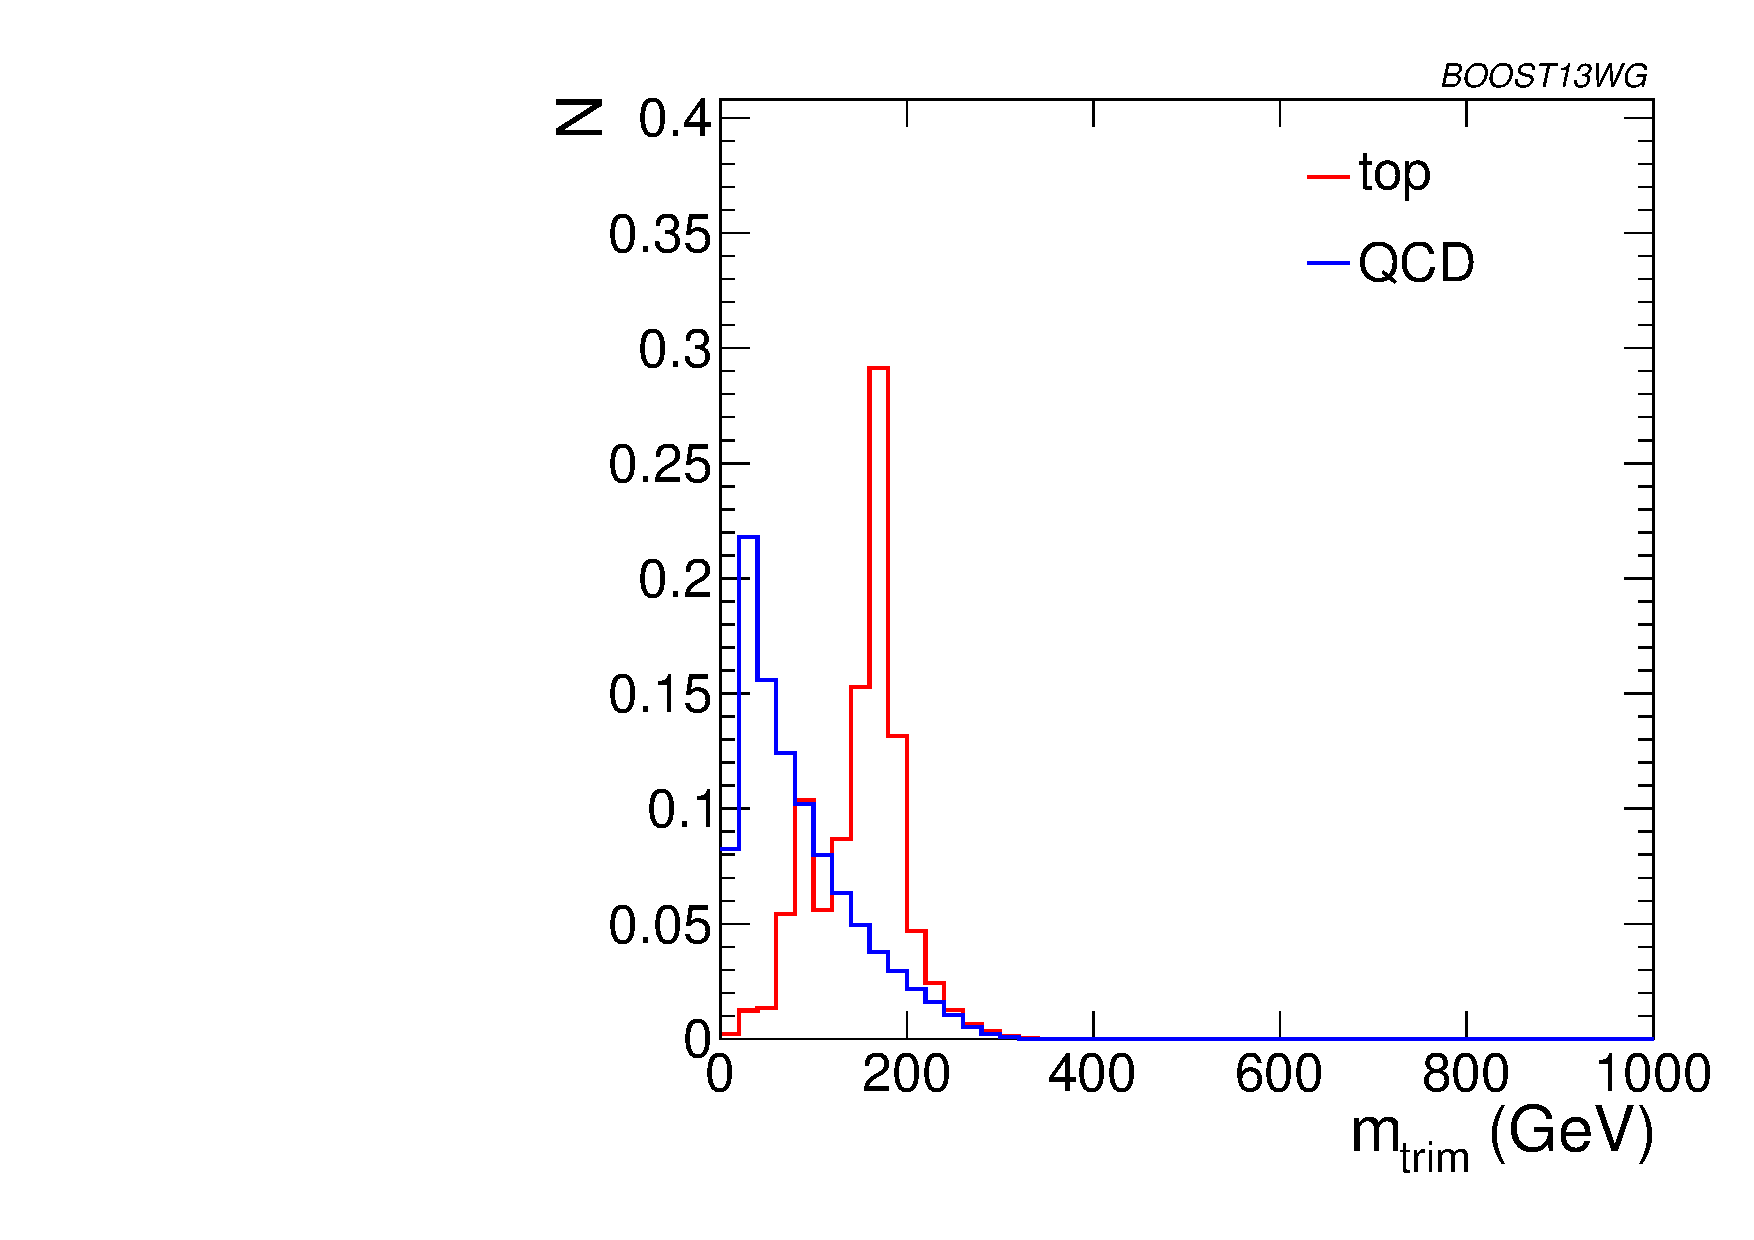
\includegraphics[width=0.245\textwidth]{./Figures/TTagging/single_variable/pT.600GeV.R.0.8/h_trim_pT_0_6.pdf}}
\subfigure[prune, \pt = 1.5-1.6 \TeV]{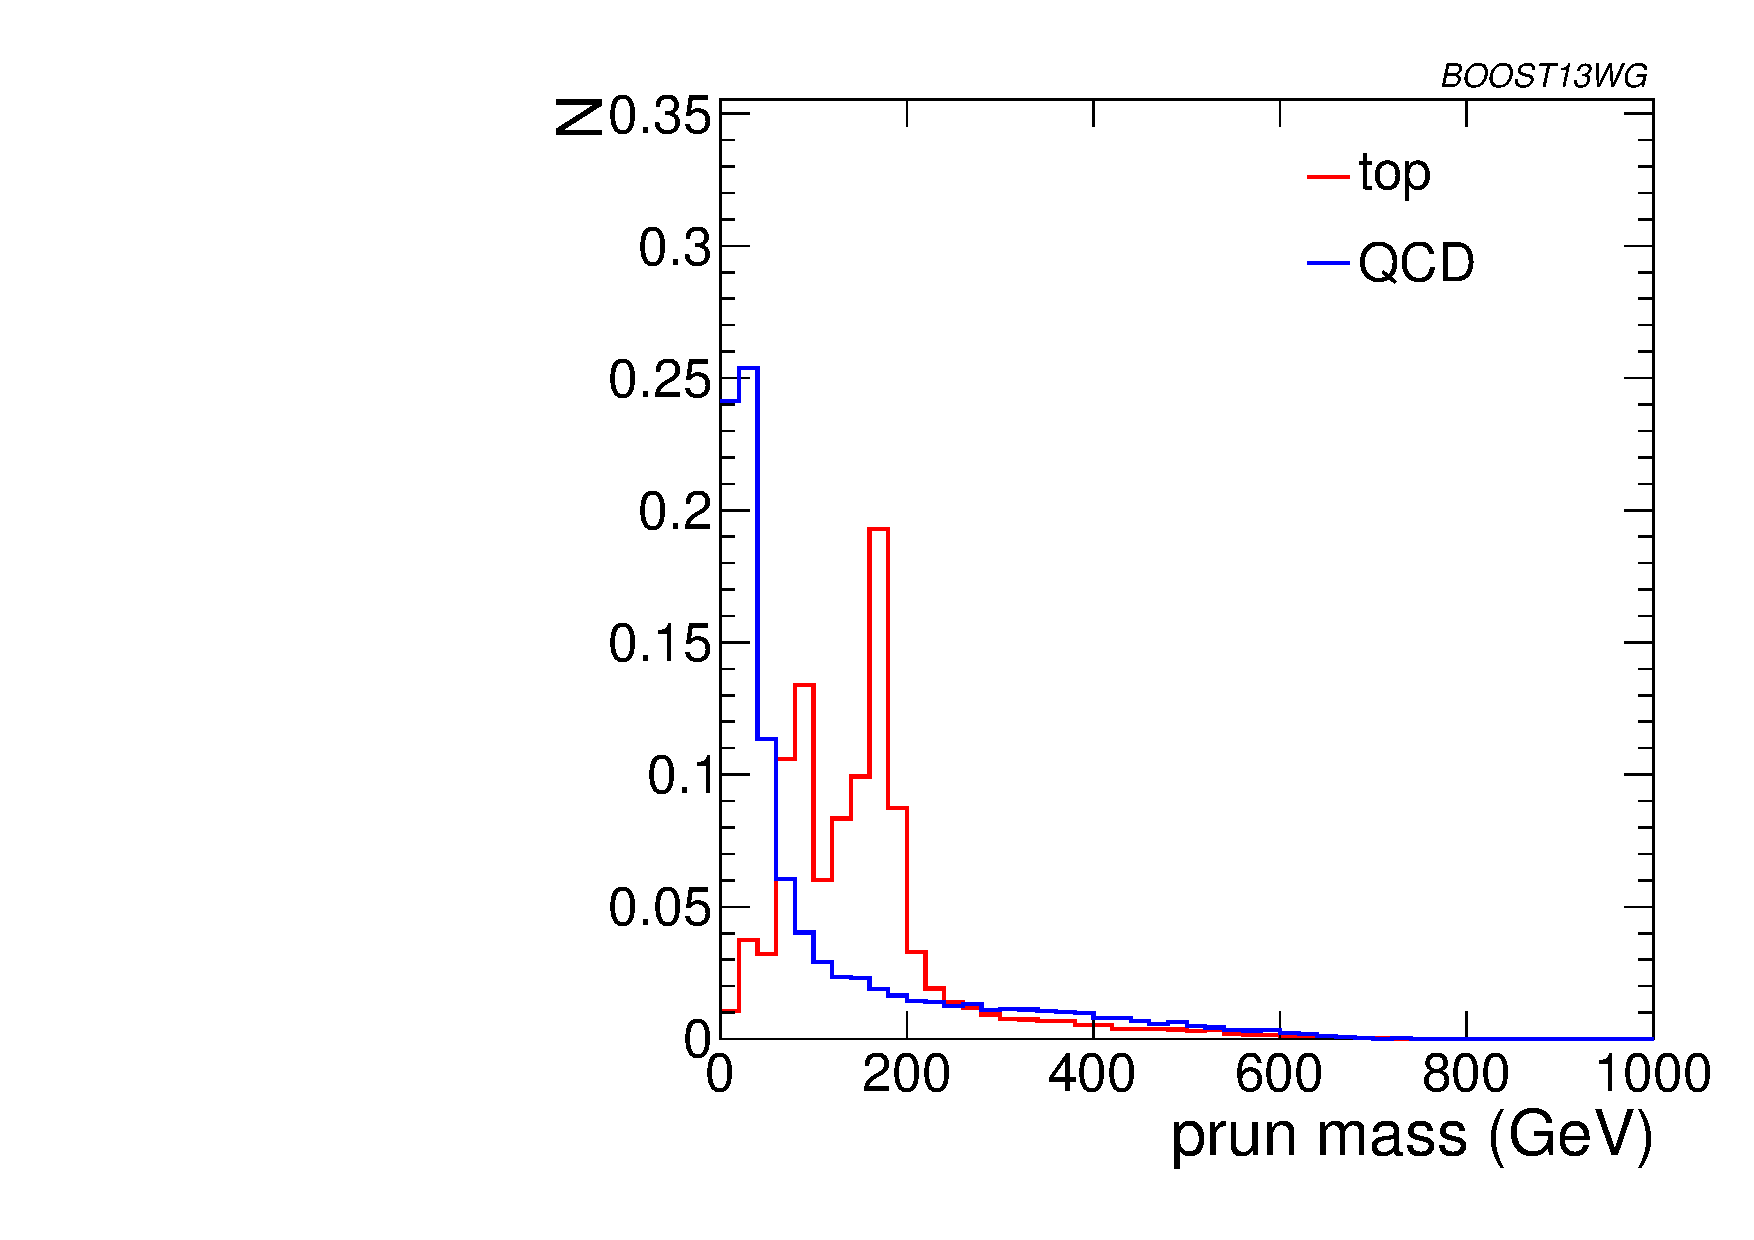
\includegraphics[width=0.245\textwidth]{./Figures/TTagging/single_variable/pT.1.5TeV.R.0.8/h_prun_pT_1_5.pdf}}
\subfigure[trim, \pt = 1.5-1.6 \TeV]{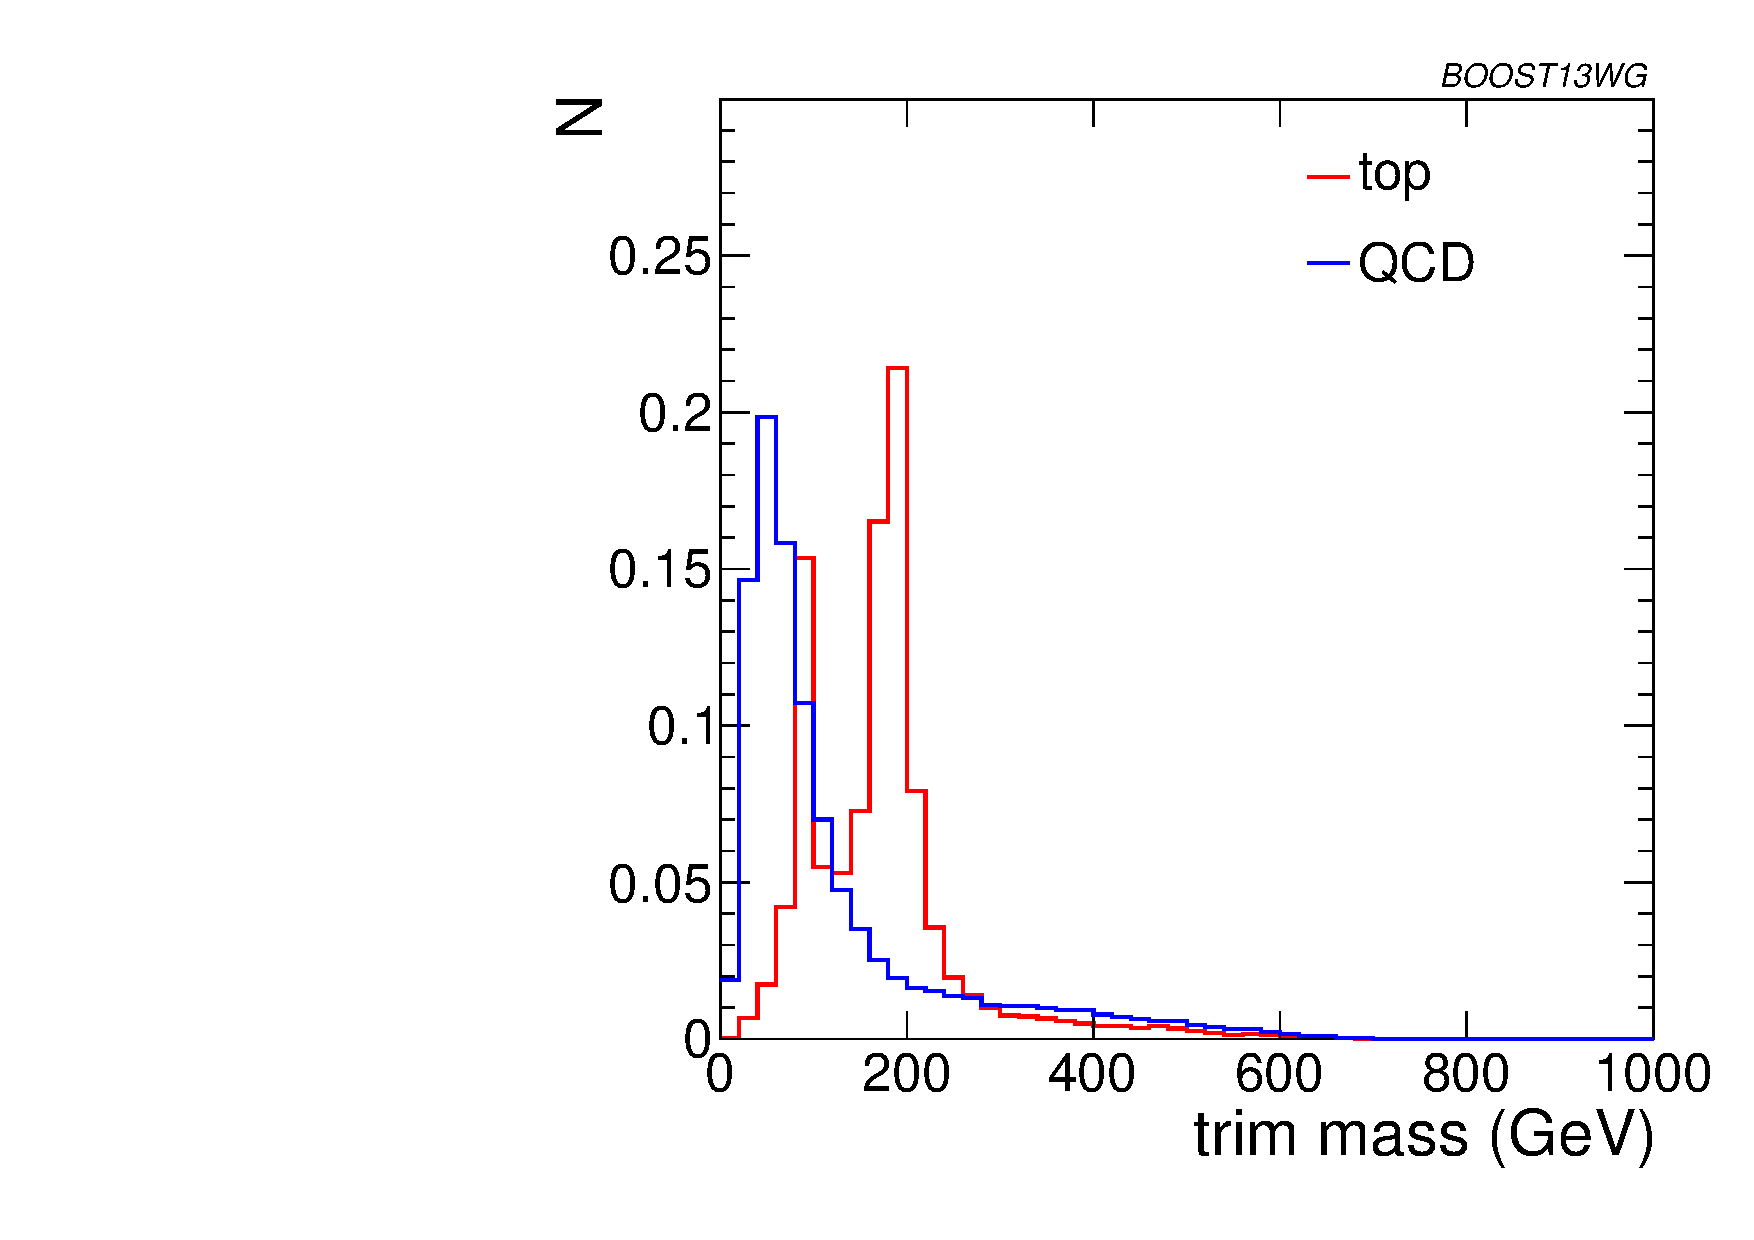
\includegraphics[width=0.245\textwidth]{./Figures/TTagging/single_variable/pT.1.5TeV.R.0.8/h_trim_pT_1_5.pdf}}
\caption{Comparison of top mass reconstruction with the Johns Hopkins (JH), HEPTopTaggers (HEP), pruning, and trimming at different \pt using the \antikt algorithm, $R=0.8$. Each histogram is shown for the working point optimized for best performance with $m_t$ in the $0.3$-$0.35$ signal efficiency bin, and is normalized to the fraction of events passing the tagger.}
\label{fig:topmass_histogram_HEP_JH_pT}
\end{figure*}

We also see in Figure~\ref{fig:single_variable_ROC_topmass} that the top mass from the JH tagger and the HEPTopTagger has superior performance relative to either of the grooming algorithms; this is because  the pruning and trimming algorithms do not have inherent $W$-identification steps and are not optimized for this purpose. Indeed, because of the lack of a $W$-identification step, grooming algorithms are forced to strike a balance between under-grooming the jet, which broadens the signal peak due to underlying event contamination and features a larger background rate, and over-grooming the jet, which occasionally throws out the $b$-jet and preserves only the $W$ components inside the jet. We demonstrate this effect in Figures~\ref{fig:topmass_histogram_HEP_JH} and \ref{fig:topmass_histogram_HEP_JH_pT}, showing that with 30\% signal efficiency, the optimal performance of the tagger over-grooms a substantial fraction of the jets ($\sim20-30\%$), leading to a spurious second peak at \wmass. This effect is more pronounced at large $R$ and $\pt$, since more aggressive grooming is required in these limits to combat the increased contamination from underlying event and QCD radiation. 


In Figures~\ref{fig:ptcomparison_singleshape_top} and~\ref{fig:ptcomparison_singletopmass_top} we directly compare ROC curves for jet-shape variable performance and top-mass performance, respectively, in three different \pt bins  whilst keeping the jet radius fixed at $R=0.8$. The input parameters of the taggers, groomers and shape variables are separately optimized in each \pt bin.  One can see from Figure~\ref{fig:ptcomparison_singleshape_top} that the tagging performance of jet shapes do not change substantially with $\pt$. The variables \tauthreetwo and $\Gamma_{\rm Qjet}$ have the most variation and tend to degrade with higher $\pt$, as can be seen in Figure~\ref{fig:Qjet_comparison_pT}. This was also observed in the $W$-tagging studies in Section~\ref{sec:wtagging}, and makes sense, as higher-$\pt$ QCD jets have more, harder emissions within the jet, giving rise to substructure that fakes the signal. 
For the variable $\Gamma_{\rm Qjet}$ (again as discussed in Section~\ref{sec:wtagging}) increasing \pt leads to QCD jets with a narrower volatility distribution
due to the enhanced contribution of the ``shoulder'' region, while for the signal (top) jets the increased amount of soft radiation with increasing \pt results
in a broader volatility distribution.  This with increasing \pt the signal and background jets exhibit more similar volatility distributions, as we see explicitly
in Figures~\ref{fig:Qjet_comparison_pT} (a) and (b).  Thus $\Gamma_{\rm Qjet}$ becomes less discriminant for top identification as \pt increases.
By contrast, from Figure~\ref{fig:ptcomparison_singletopmass_top} we can see that most of the top-mass variables have superior performance at higher $\pt$, due to the radiation from the top quark becoming more collimated. The notable exception is the HEPTopTagger, which degrades at higher $\pt$, likely in part due to the background-shaping effects studied above.


\begin{figure*}
\centering
\subfigure[$C_2^{\beta=1}$]{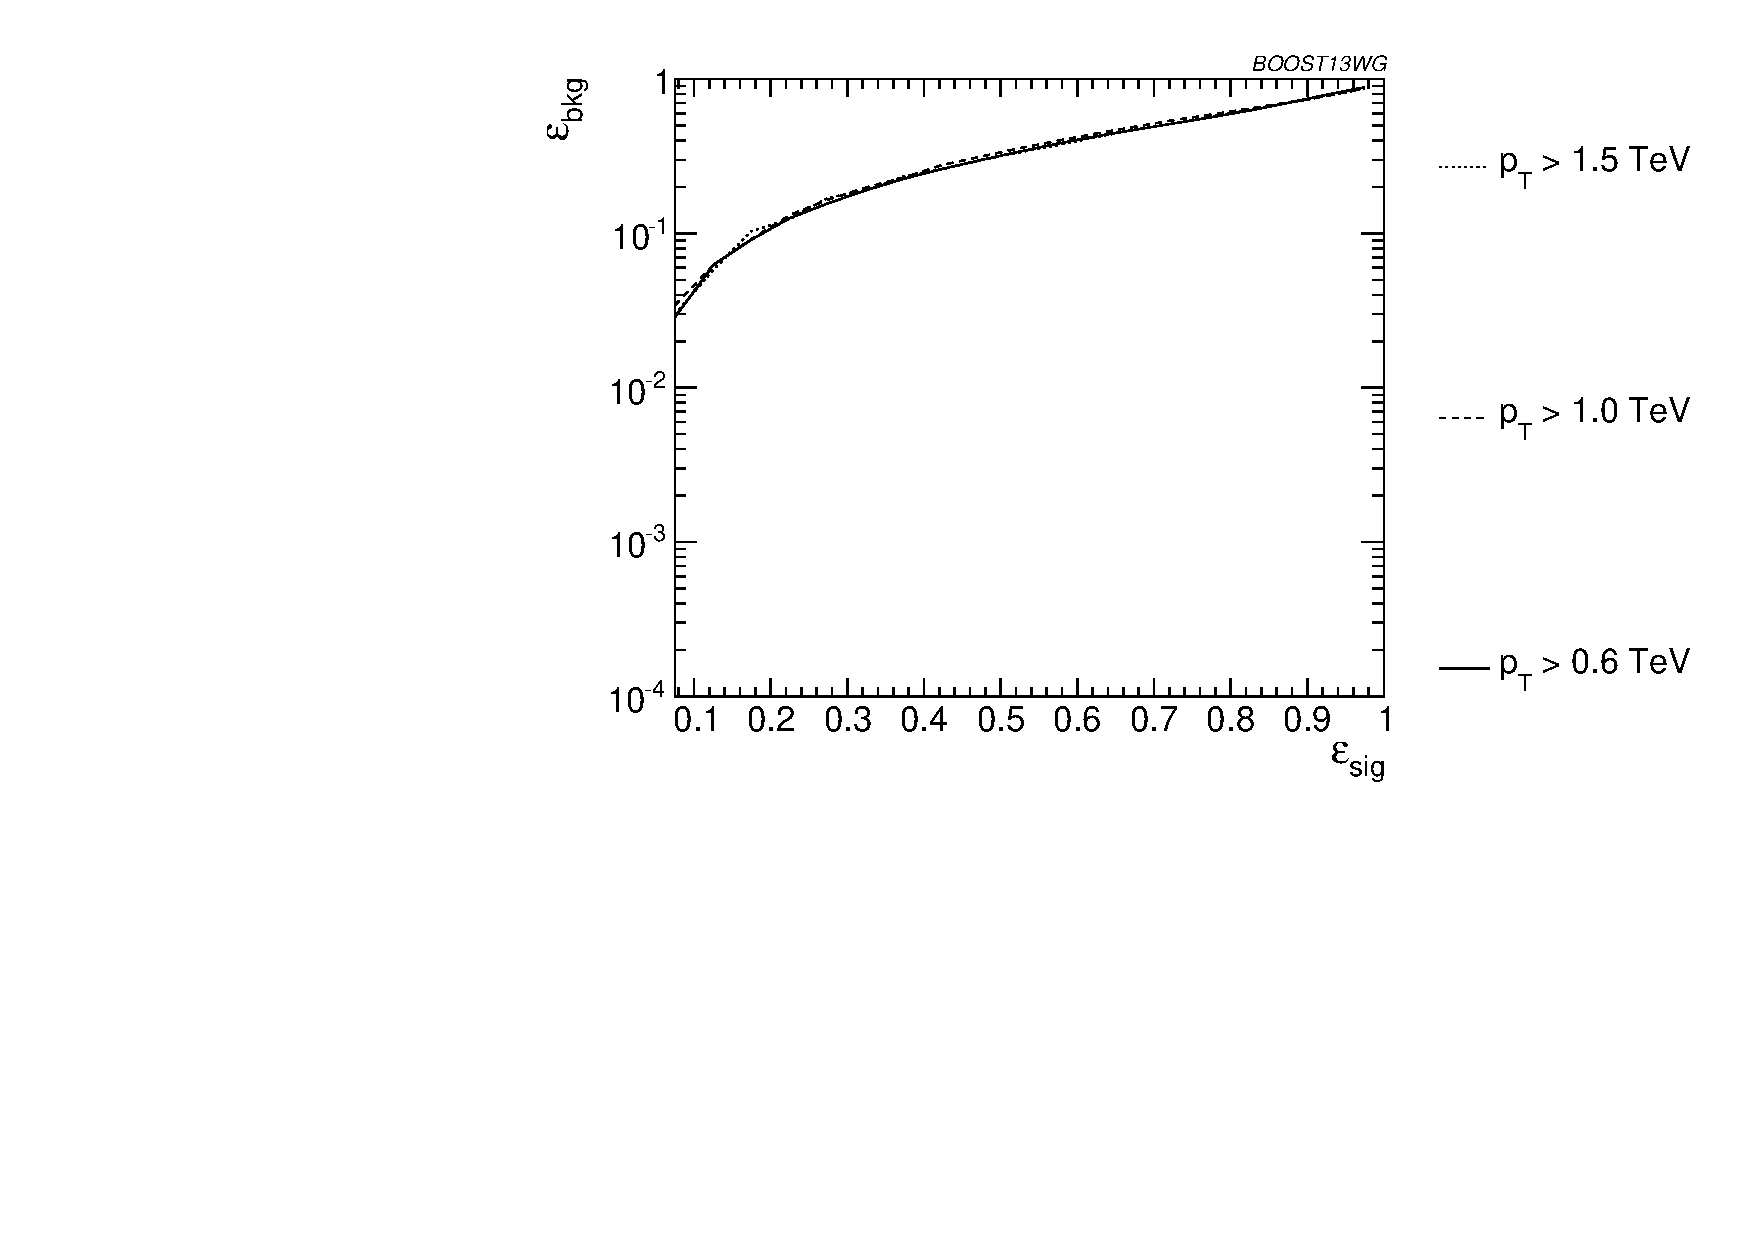
\includegraphics[width=0.48\textwidth]{./Figures/TTagging/single_variable/pT_compare/Rocs_C2b1_pTcompare.pdf}}
\subfigure[$C_3^{\beta=1}$]{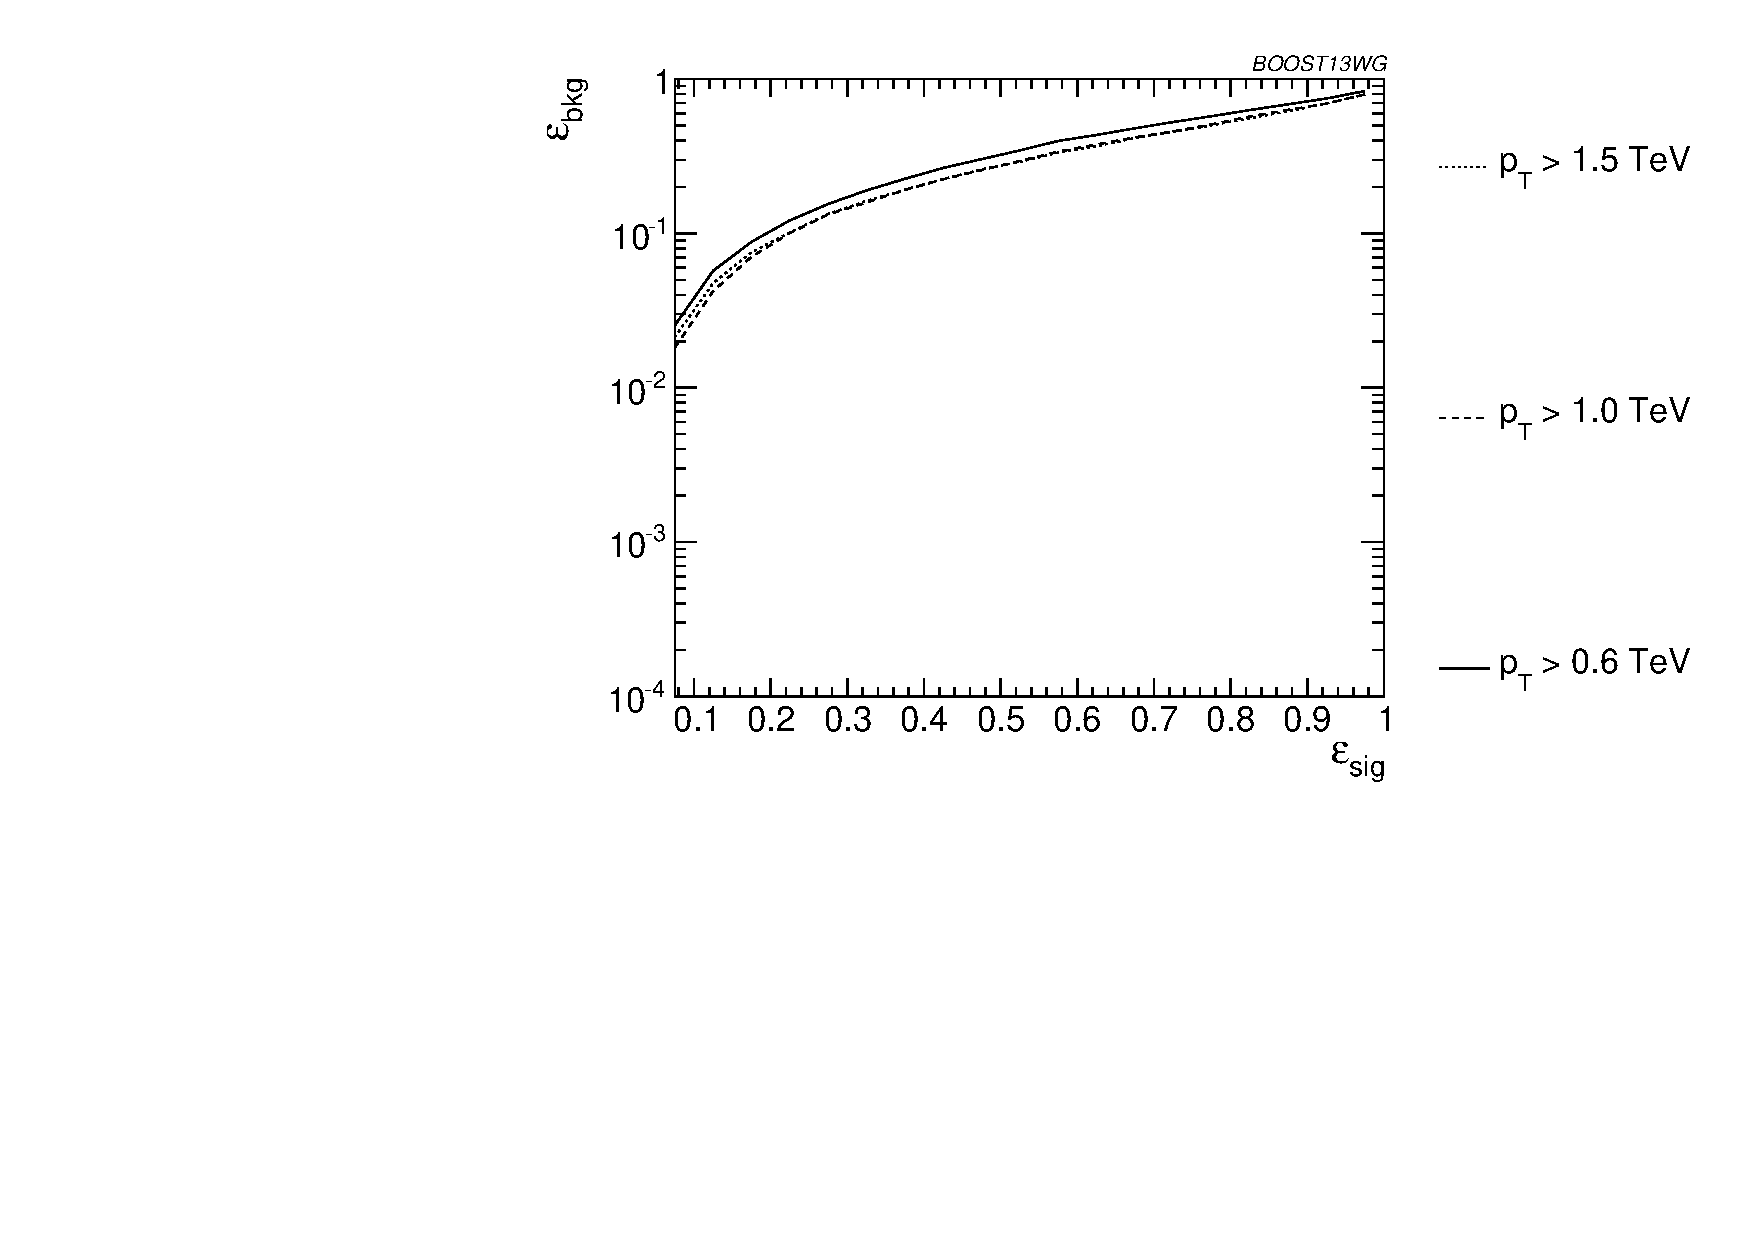
\includegraphics[width=0.48\textwidth]{./Figures/TTagging/single_variable/pT_compare/Rocs_C3b1_pTcompare.pdf}\label{fig:ptcomparison_singleshape_top_C3}}
\subfigure[\tautwoone]{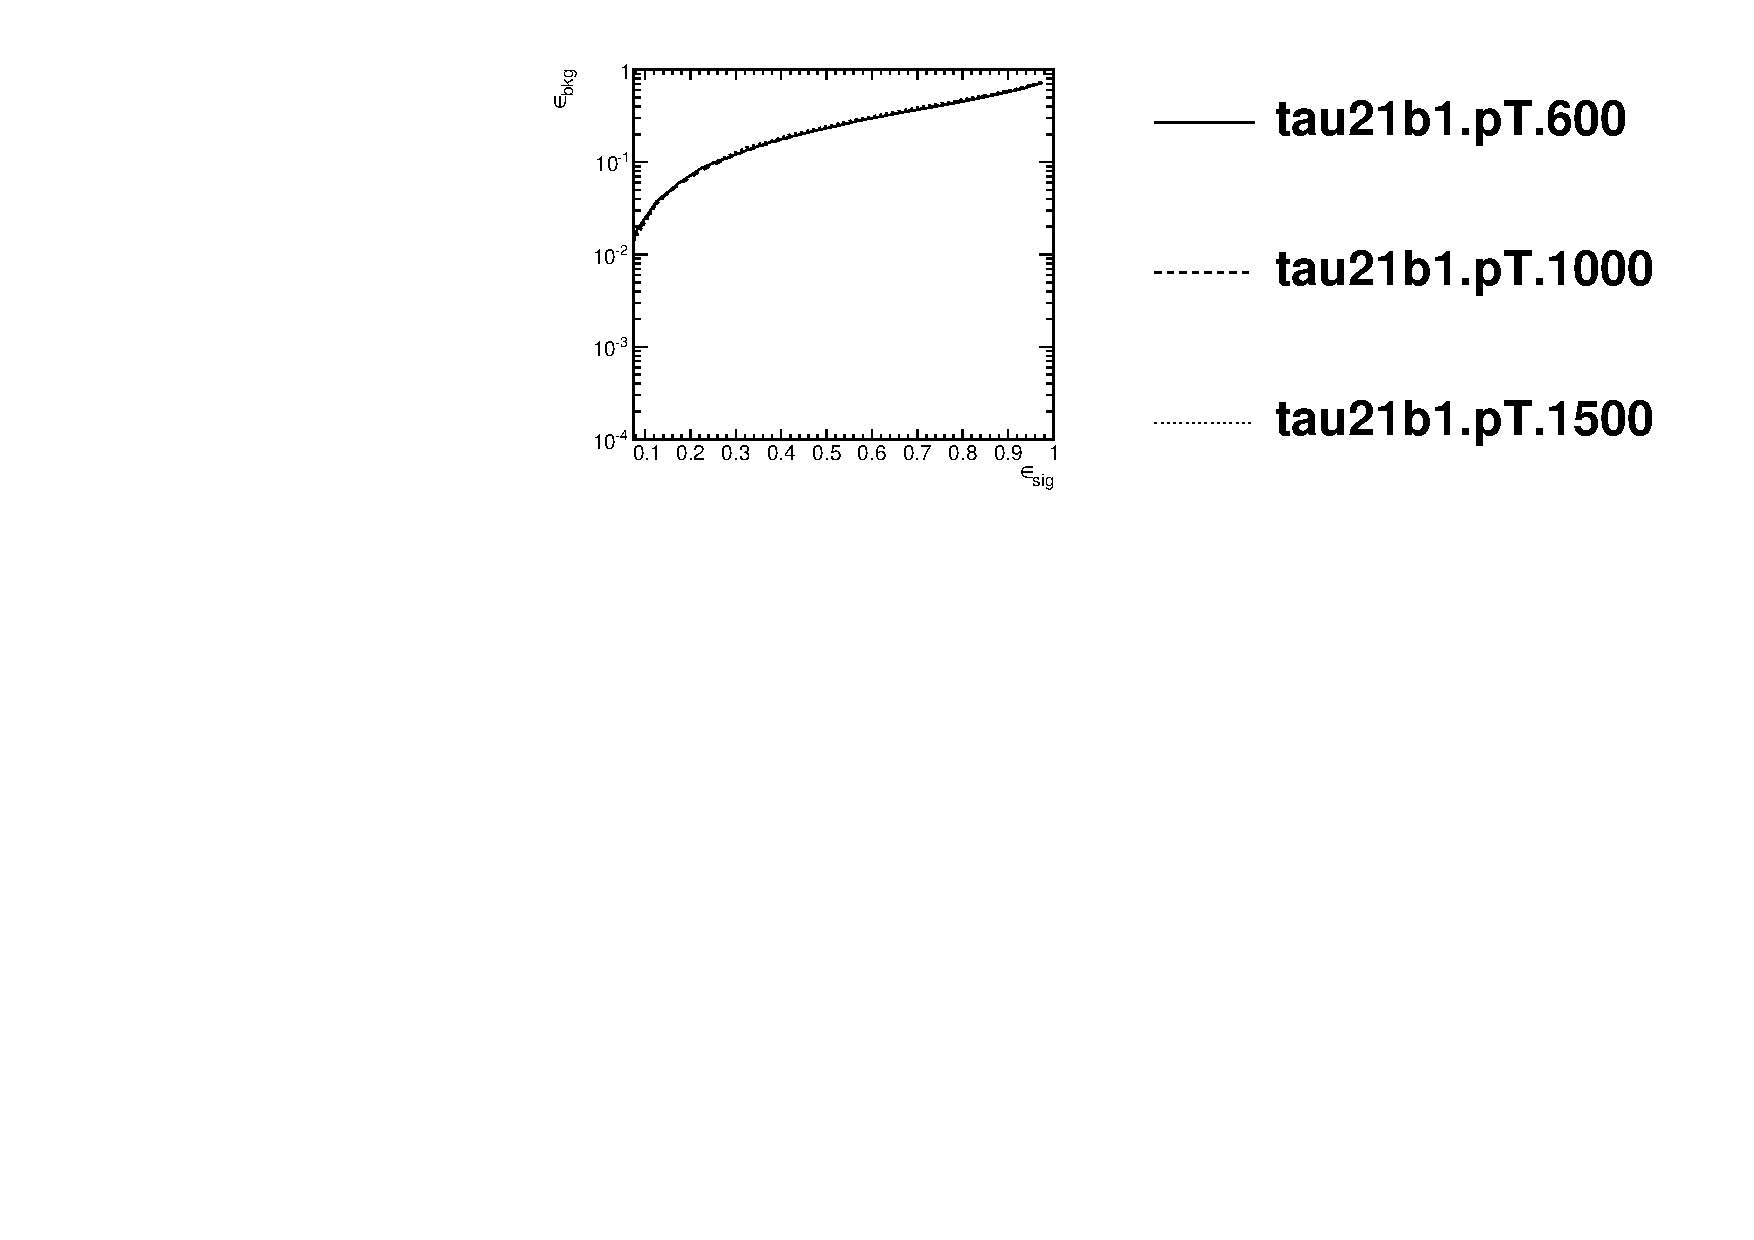
\includegraphics[width=0.48\textwidth]{./Figures/TTagging/single_variable/pT_compare/Rocs_tau21b1_pTcompare.pdf}}
\subfigure[\tauthreetwo]{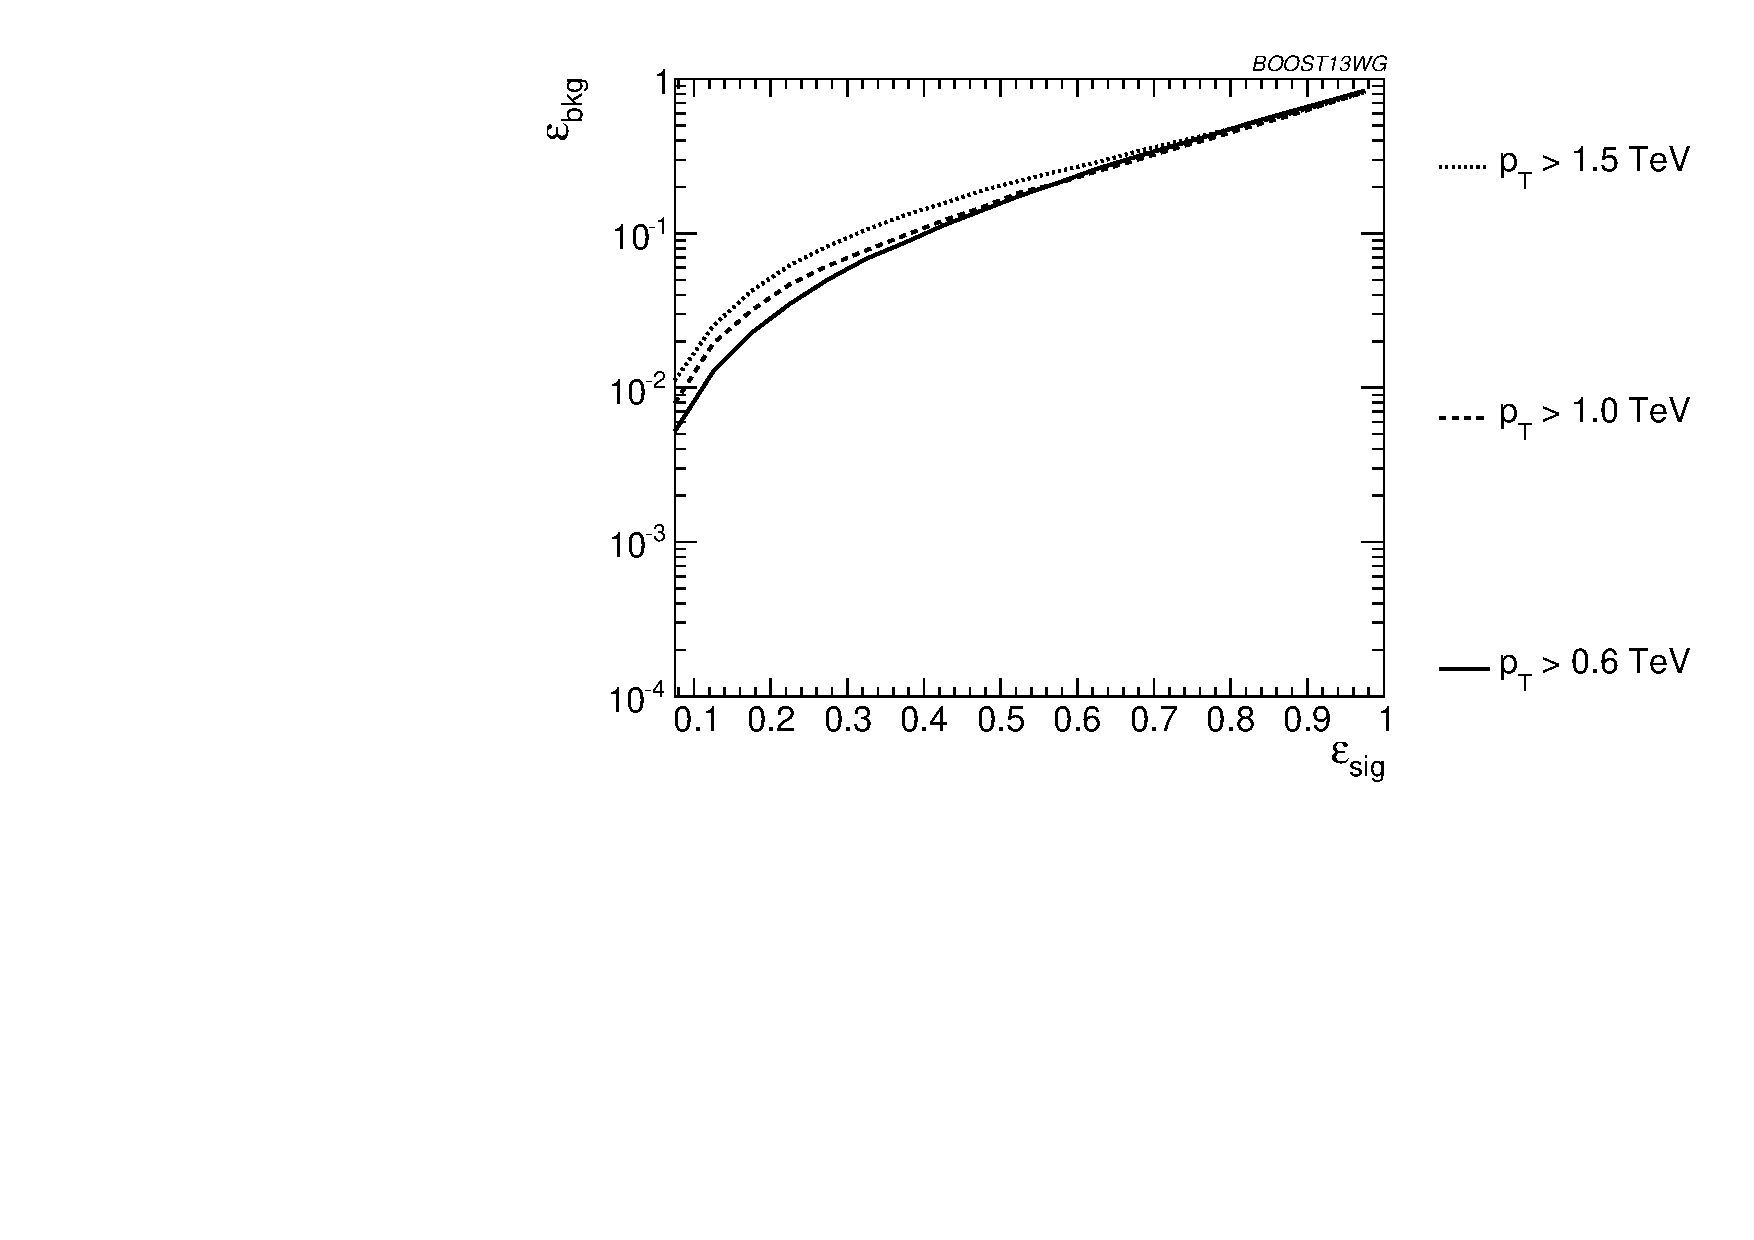
\includegraphics[width=0.48\textwidth]{./Figures/TTagging/single_variable/pT_compare/Rocs_tau32b1_pTcompare.pdf}}
\subfigure[$\Gamma_{\rm Qjet}$]{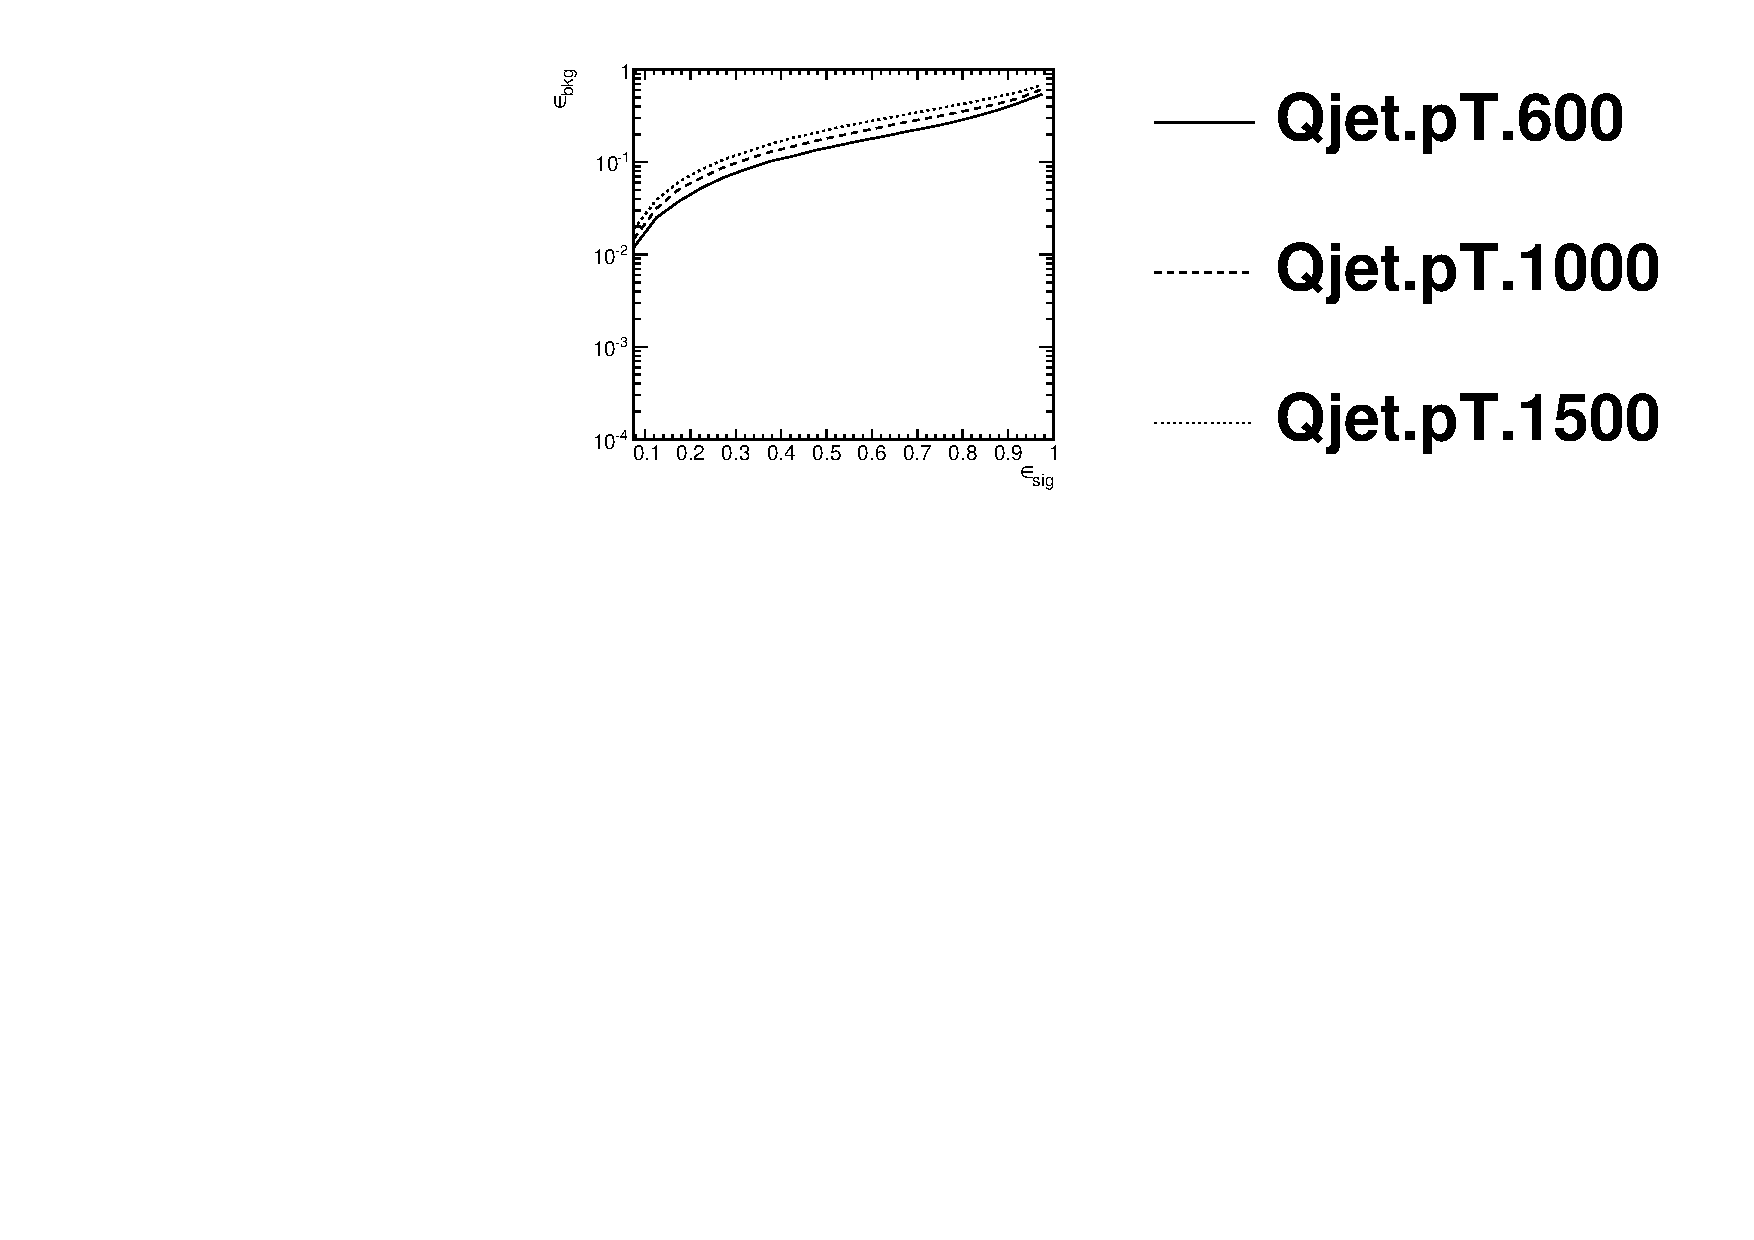
\includegraphics[width=0.48\textwidth]{./Figures/TTagging/single_variable/pT_compare/Rocs_Qjet_pTcompare.pdf}}
\caption{Comparison of individual jet shape performance at different \pt using the anti-\kT $R=0.8$ algorithm.}
\label{fig:ptcomparison_singleshape_top}
\end{figure*}


\begin{figure*}
\centering
\subfigure[HEPTopTagger $m_t$]{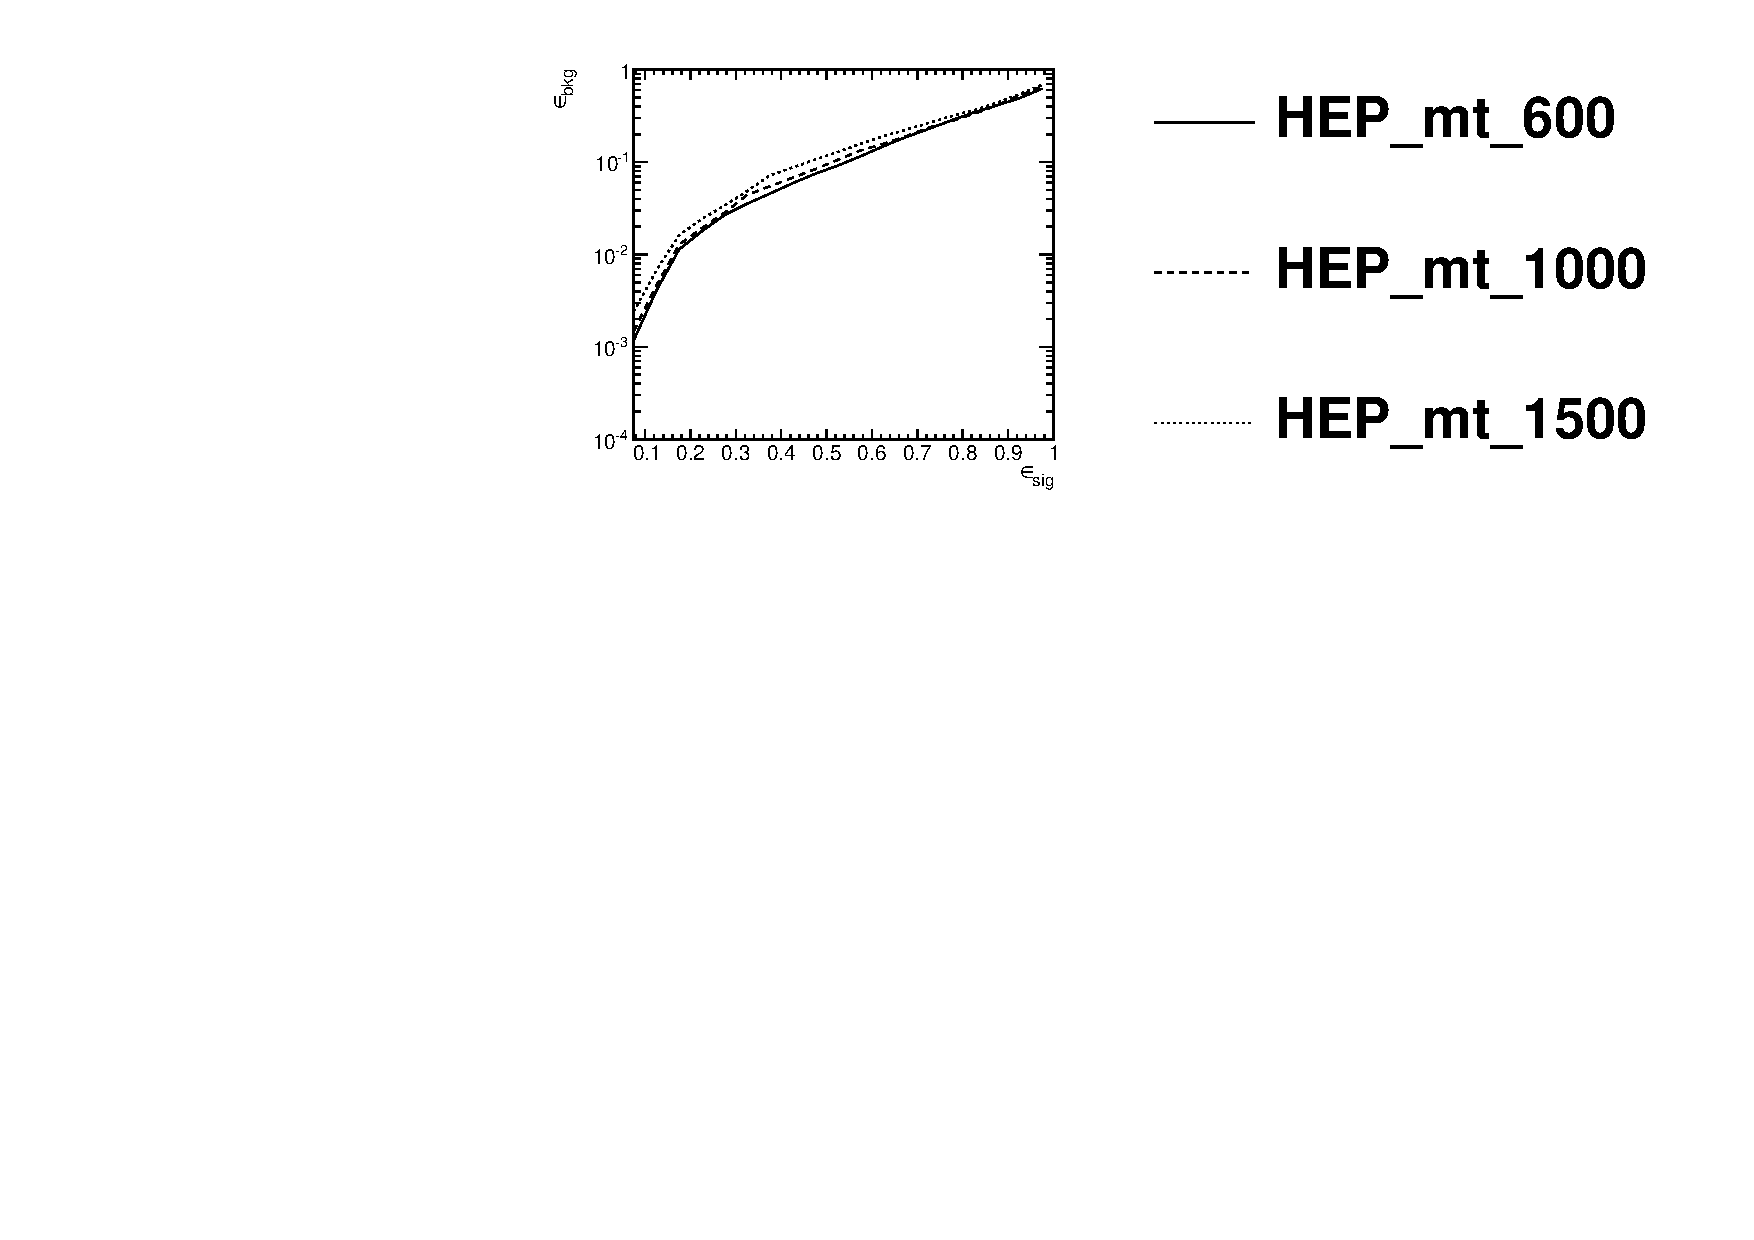
\includegraphics[width=0.48\textwidth]{./Figures/TTagging/single_variable/pT_compare/Rocs_HEP_mt_pTcompare.pdf}}
\subfigure[Johns Hopkins Tagger $m_t$]{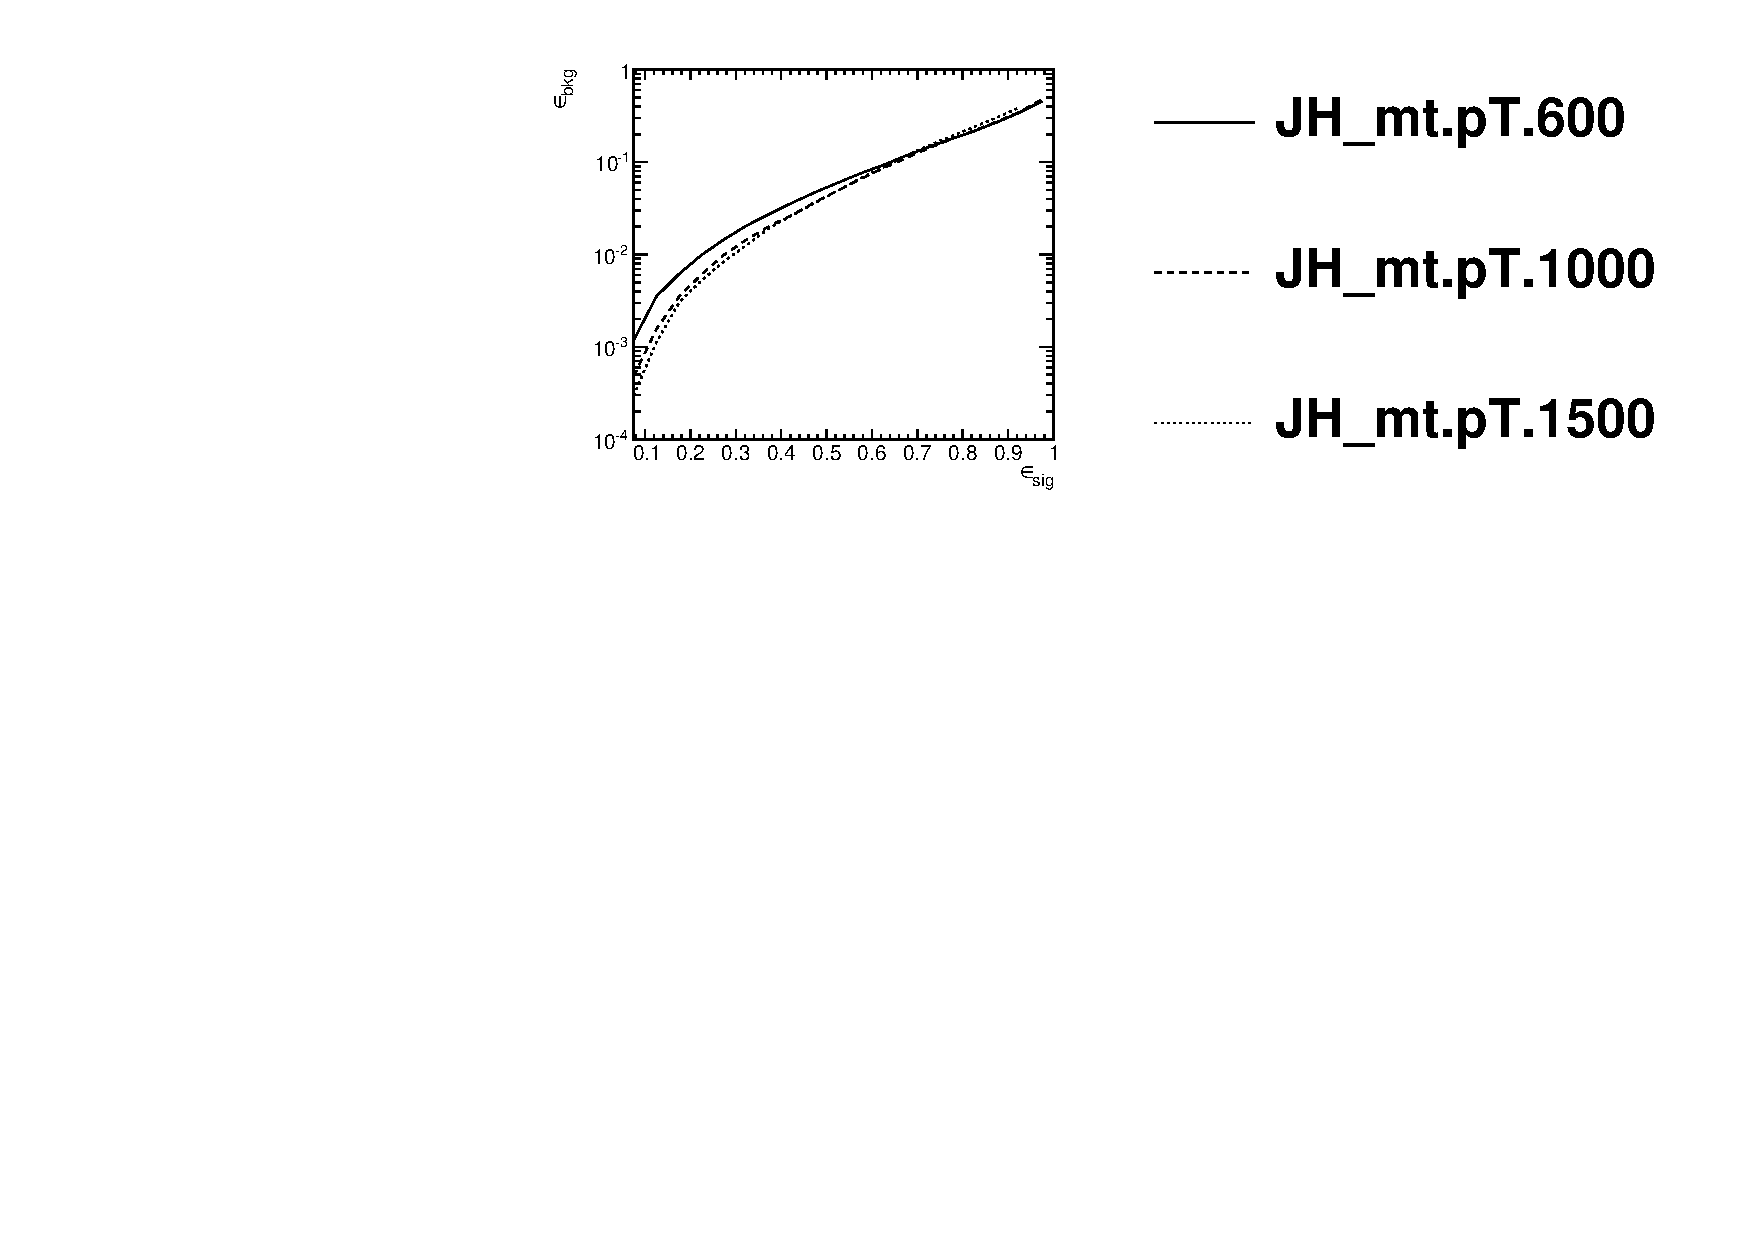
\includegraphics[width=0.48\textwidth]{./Figures/TTagging/single_variable/pT_compare/Rocs_JH_mt_pTcompare.pdf}}
\subfigure[Pruning $m_t$]{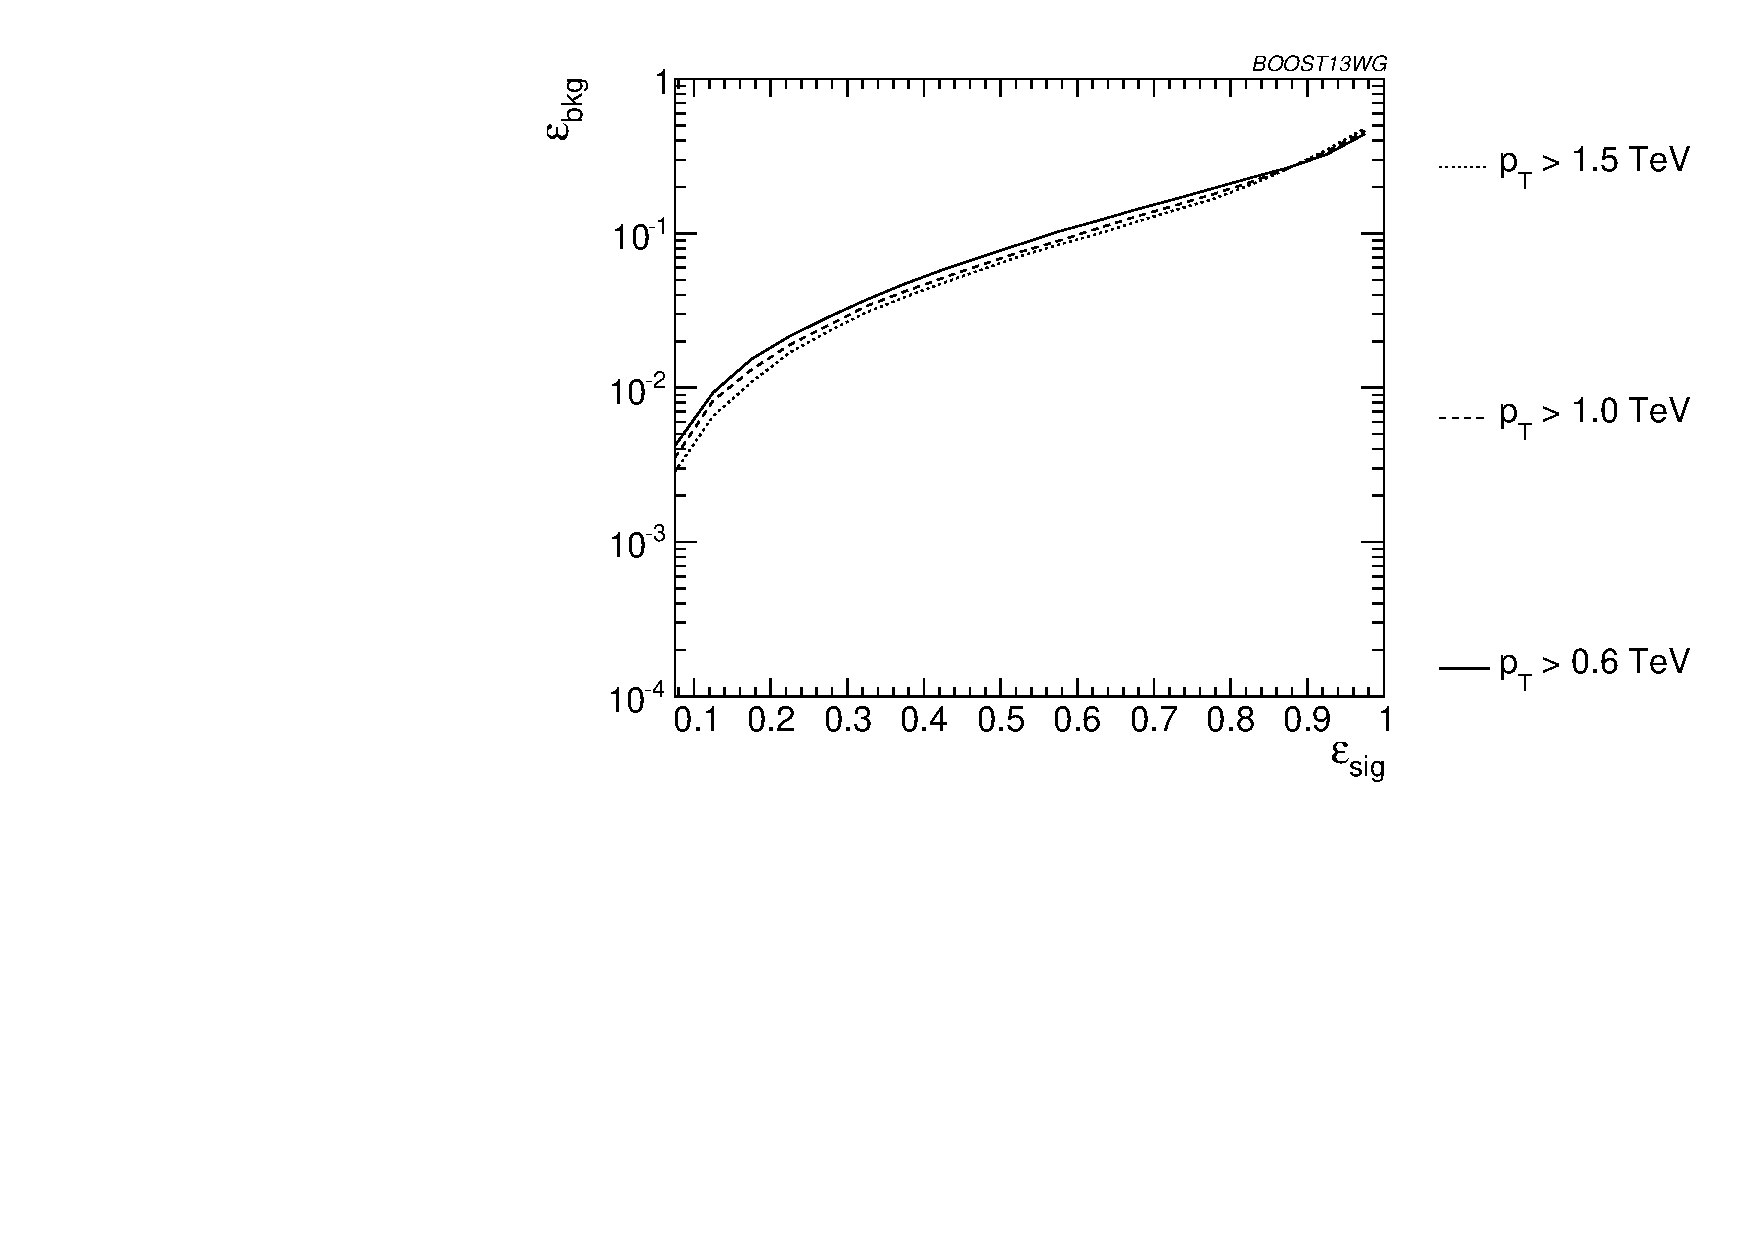
\includegraphics[width=0.48\textwidth]{./Figures/TTagging/single_variable/pT_compare/Rocs_prune_pTcompare.pdf}}
\subfigure[Trimming $m_t$]{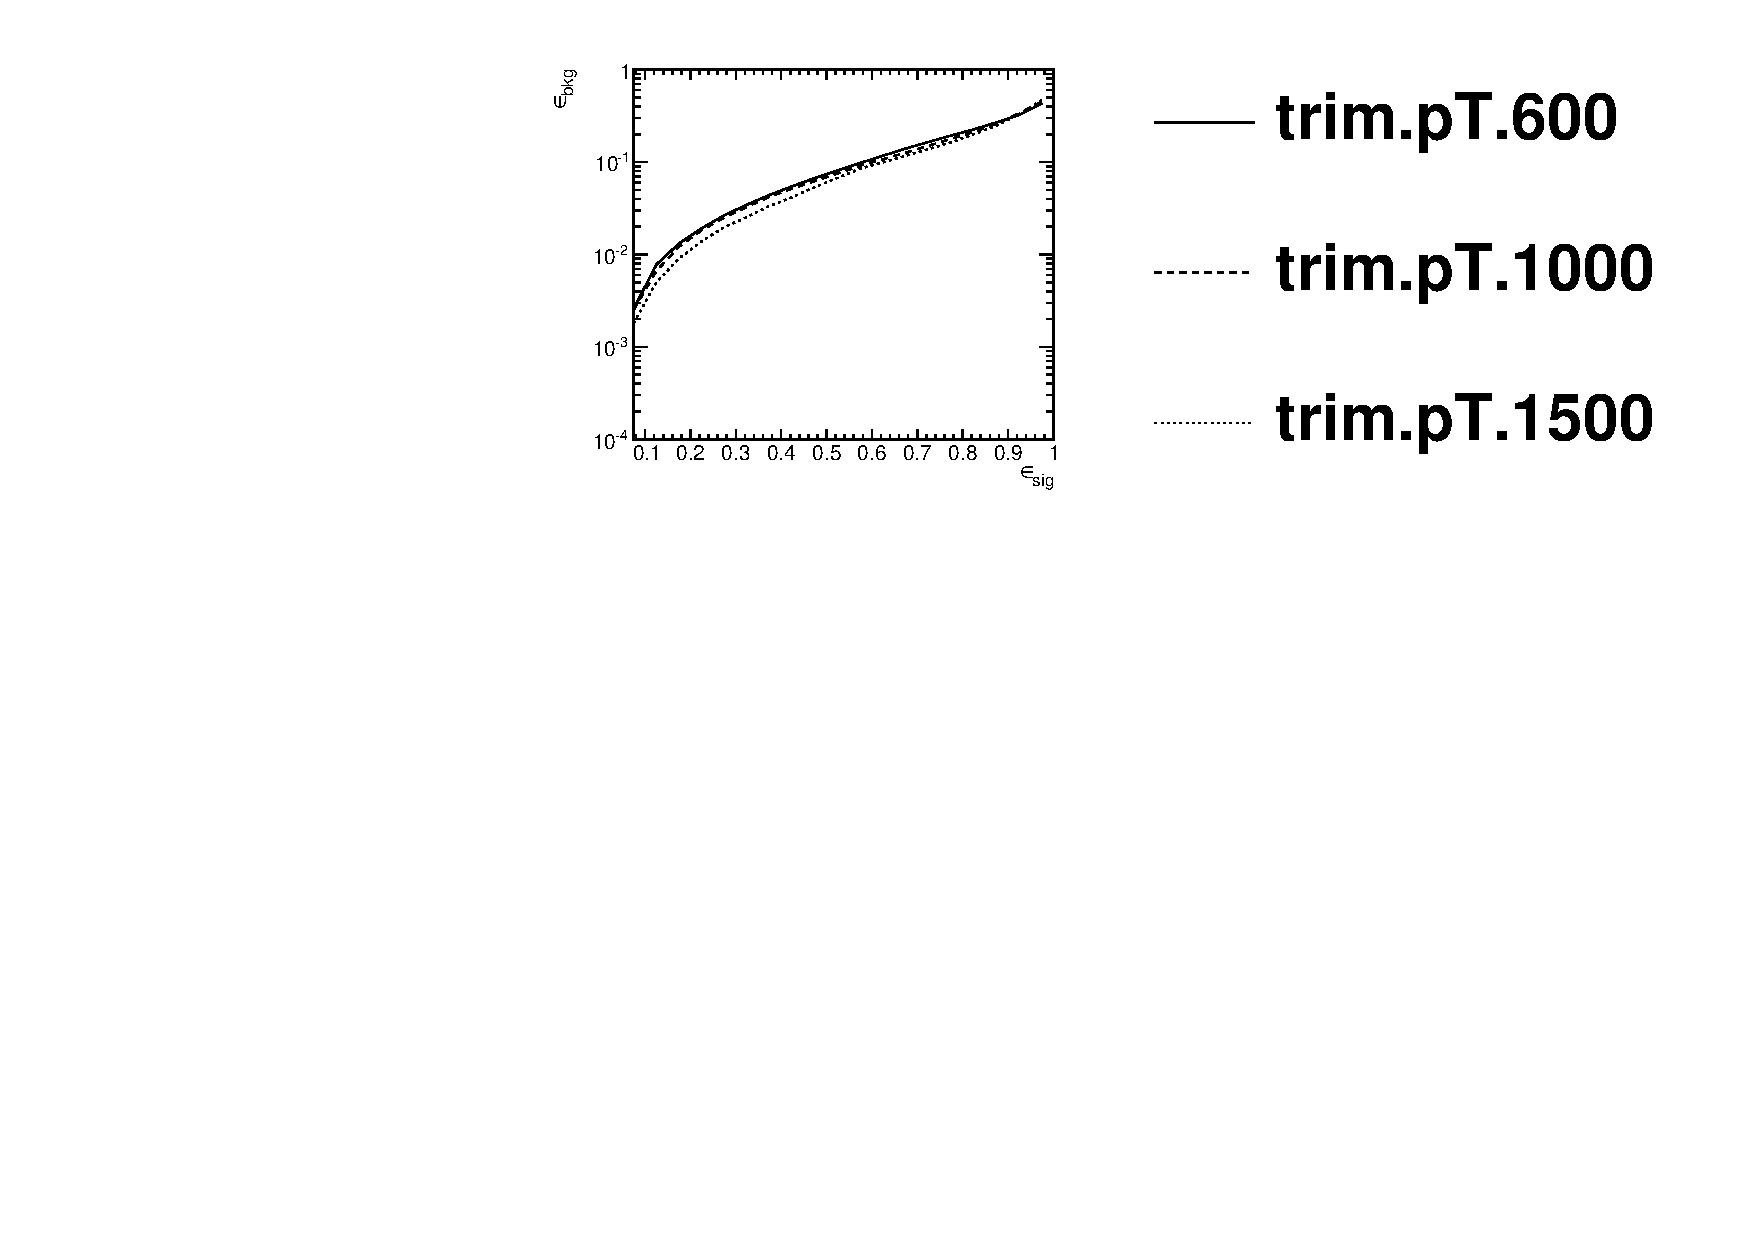
\includegraphics[width=0.48\textwidth]{./Figures/TTagging/single_variable/pT_compare/Rocs_trim_pTcompare.pdf}}
\caption{Comparison of top mass performance of different taggers at different \pt using the anti-\kT R=0.8 algorithm.}
\label{fig:ptcomparison_singletopmass_top}
\end{figure*}

\begin{figure*}
\centering
\subfigure[$\Gamma_{\rm Qjet}$, \pt = 600-700 \GeV]{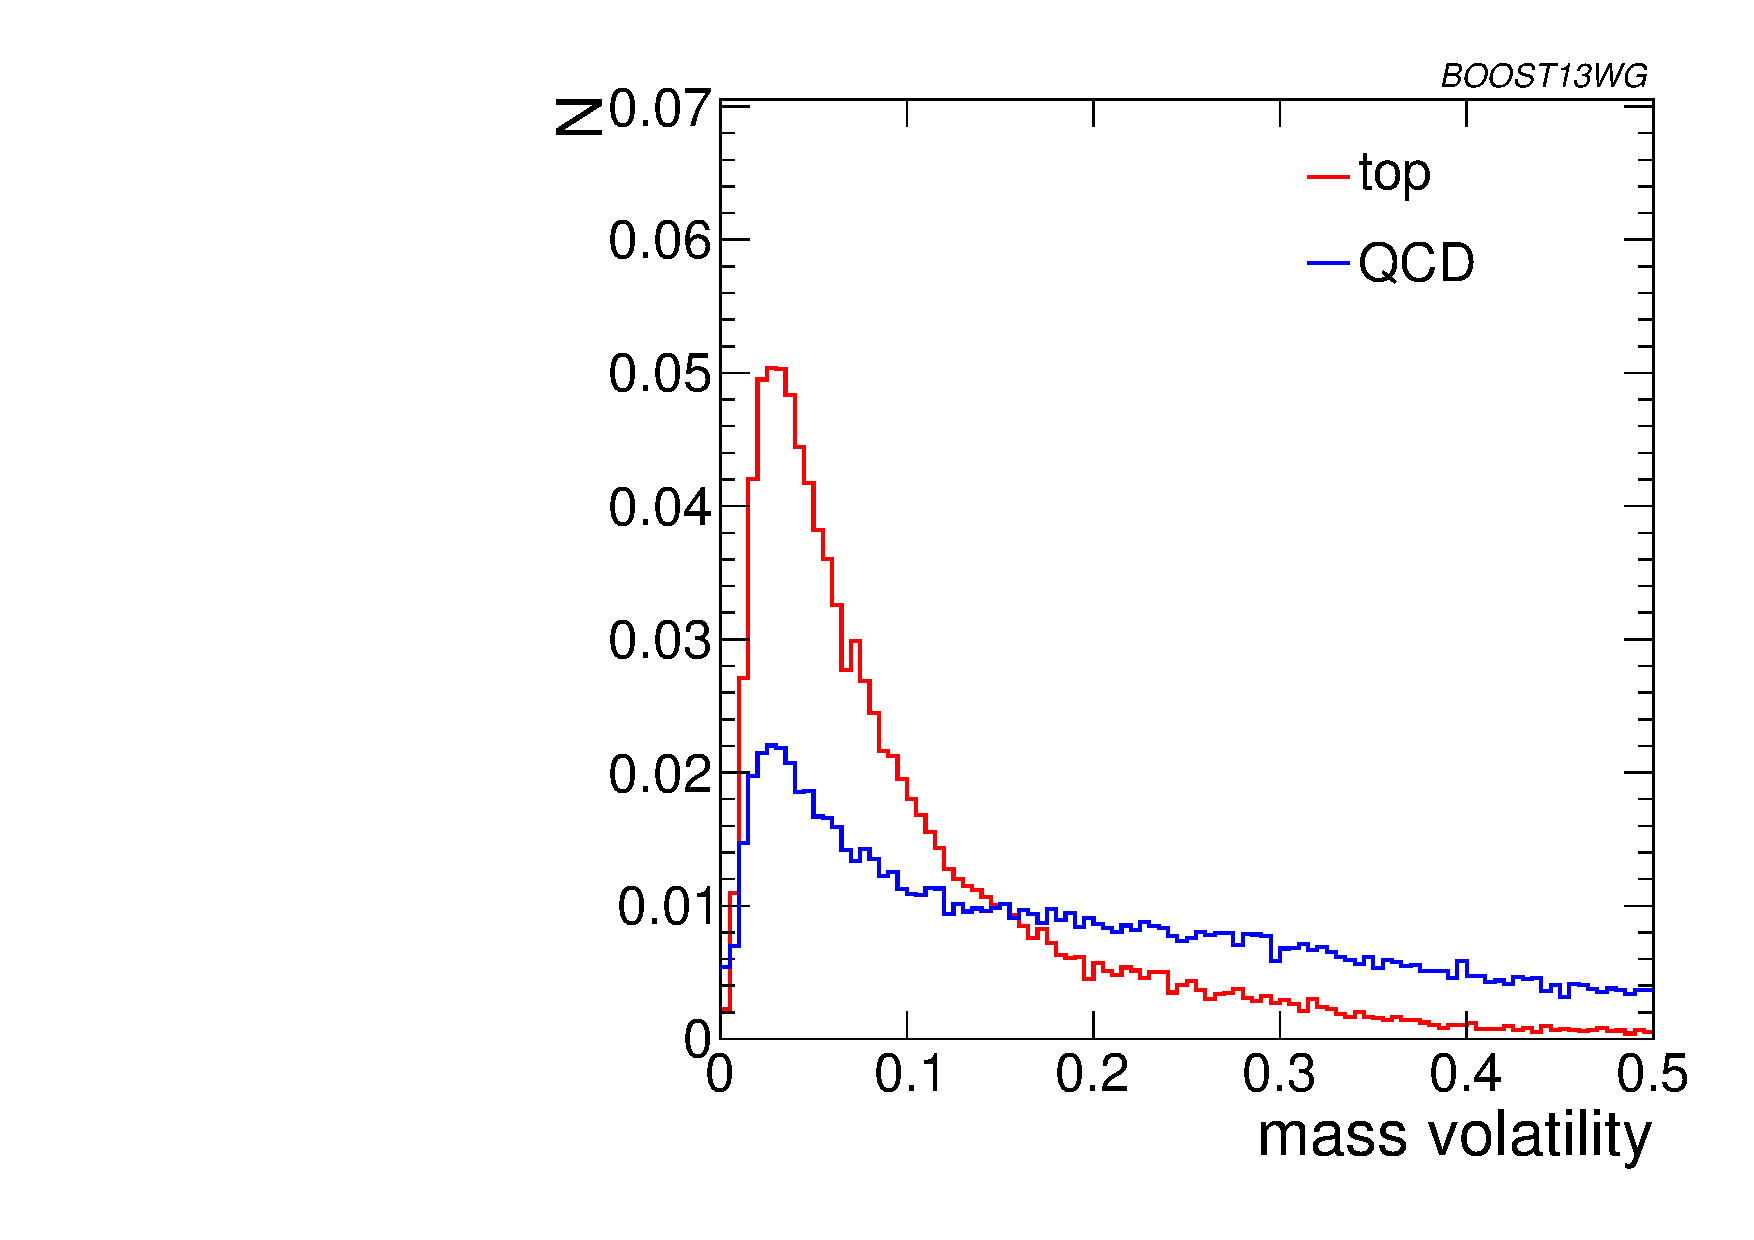
\includegraphics[width=0.245\textwidth]{./Figures/TTagging/single_variable/pT.600GeV.R.0.8/h_qjetVol_pT_0_6.pdf}}
\subfigure[$\Gamma_{\rm Qjet}$, \pt = 1.5-1.6 \TeV]{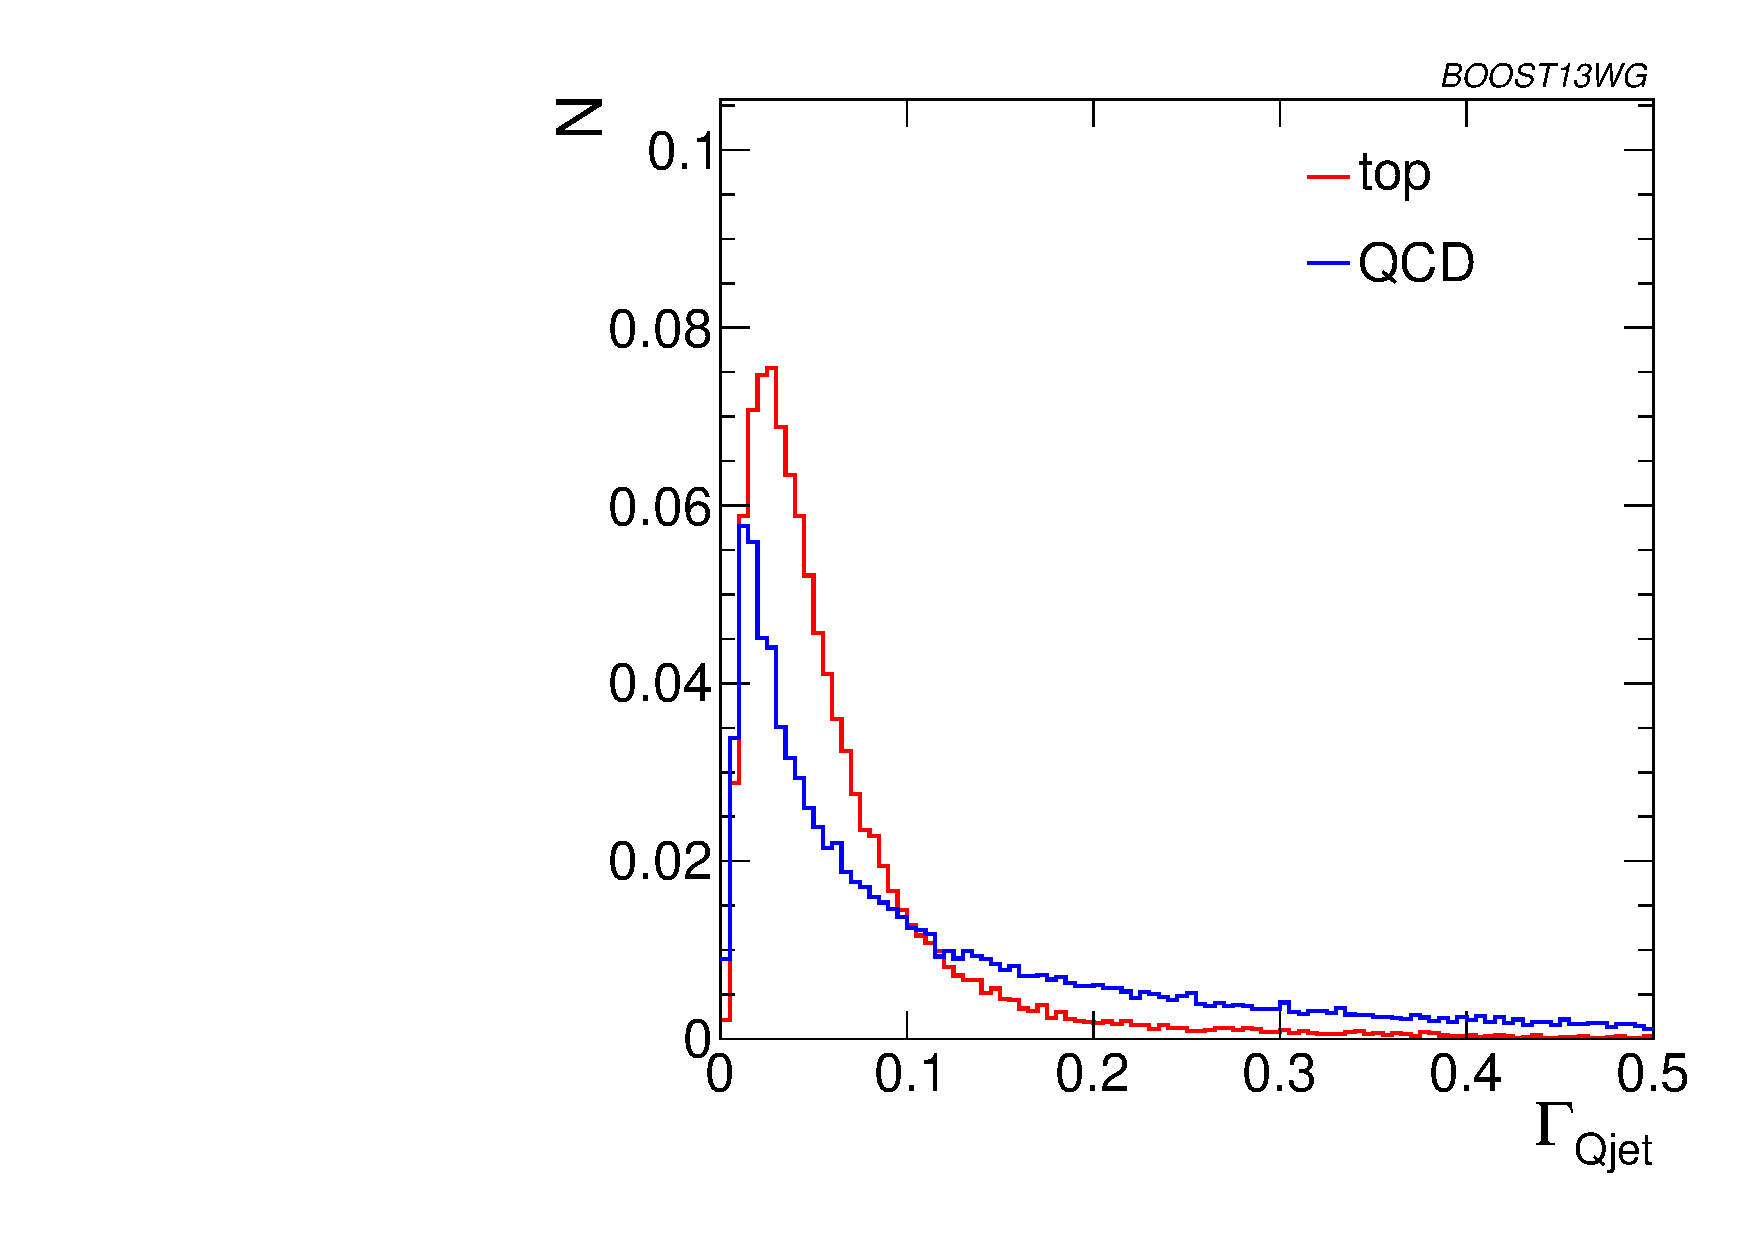
\includegraphics[width=0.245\textwidth]{./Figures/TTagging/single_variable/pT.1.5TeV.R.0.8/h_qjetVol_R_0_8.pdf}}
\subfigure[\tauthreetwo, \pt = 600-700 \GeV]{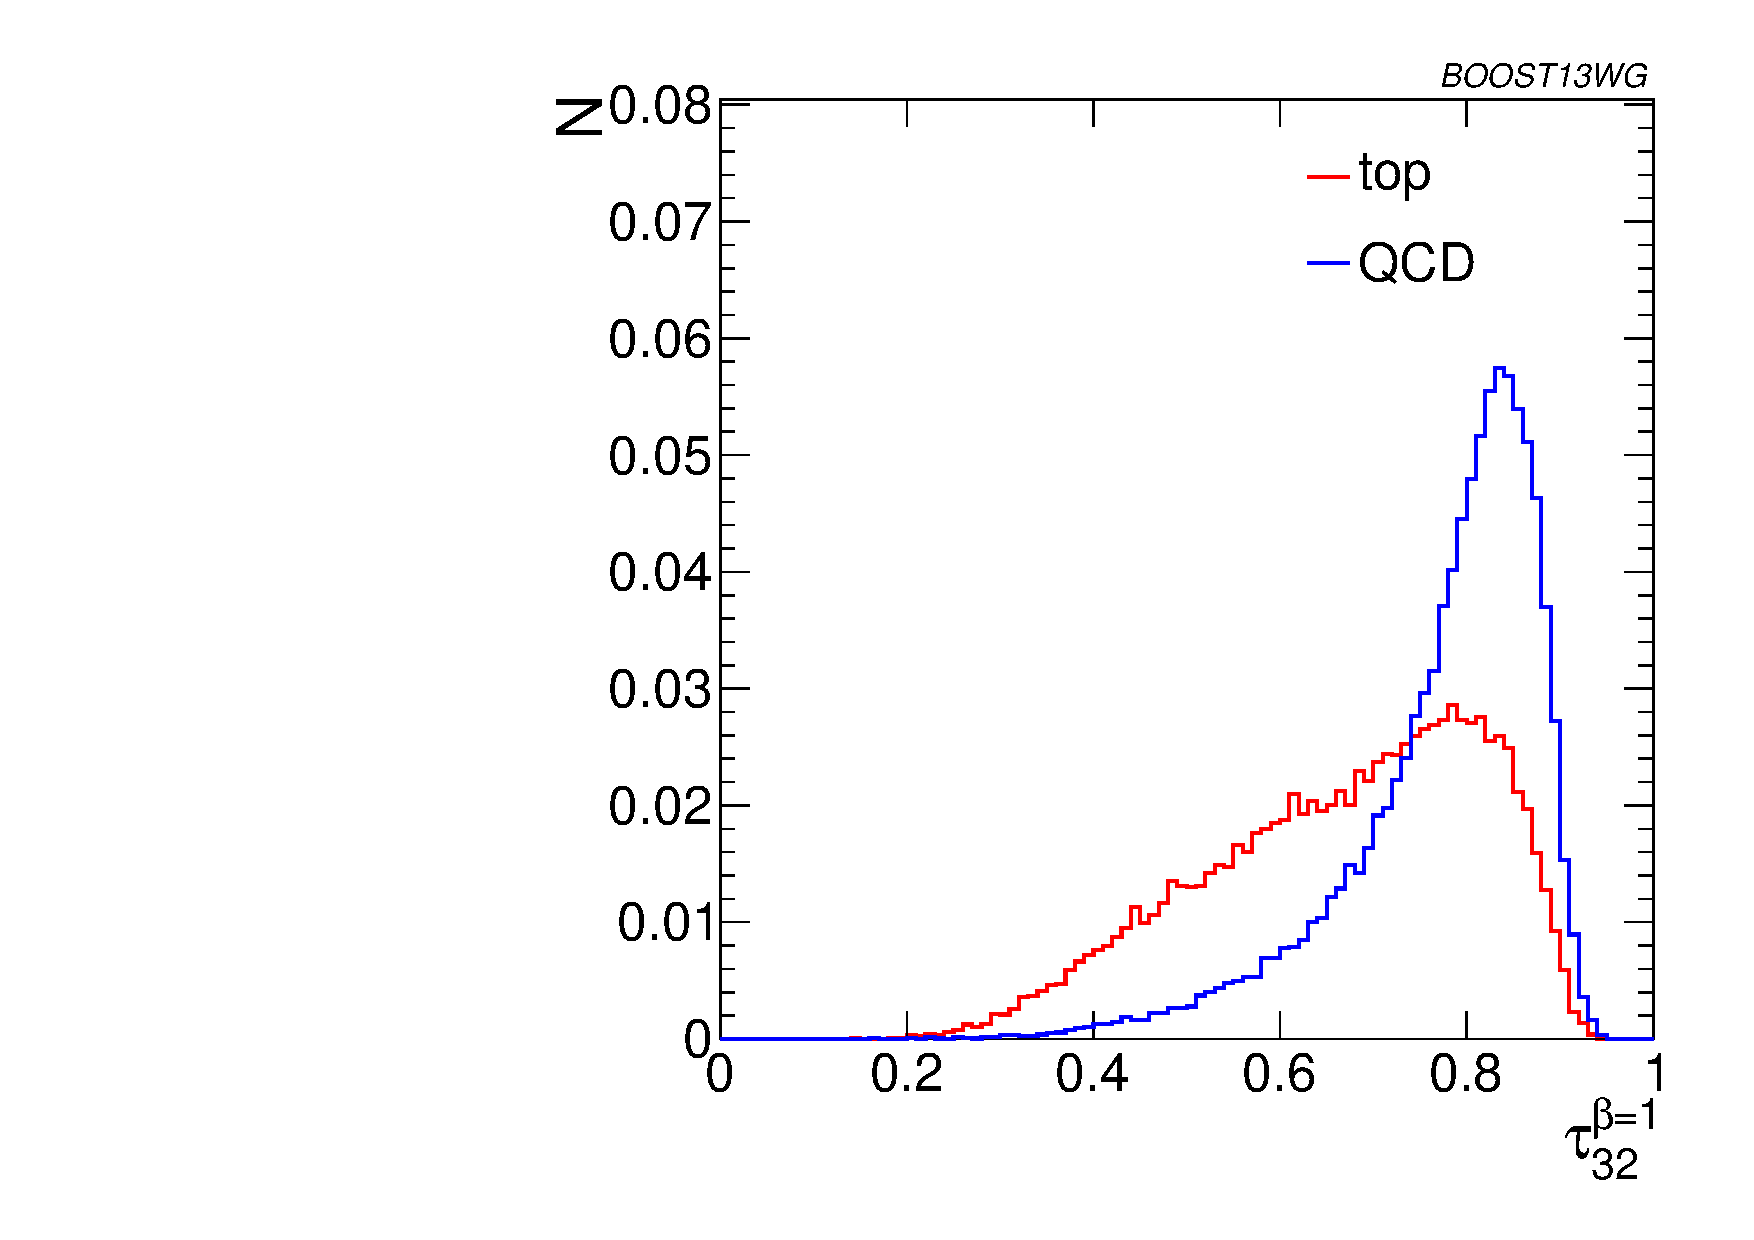
\includegraphics[width=0.245\textwidth]{./Figures/TTagging/single_variable/pT.600GeV.R.0.8/h_tau32b1_pT_0_6.pdf}}
\subfigure[\tauthreetwo, \pt = 1.5-1.6 \TeV]{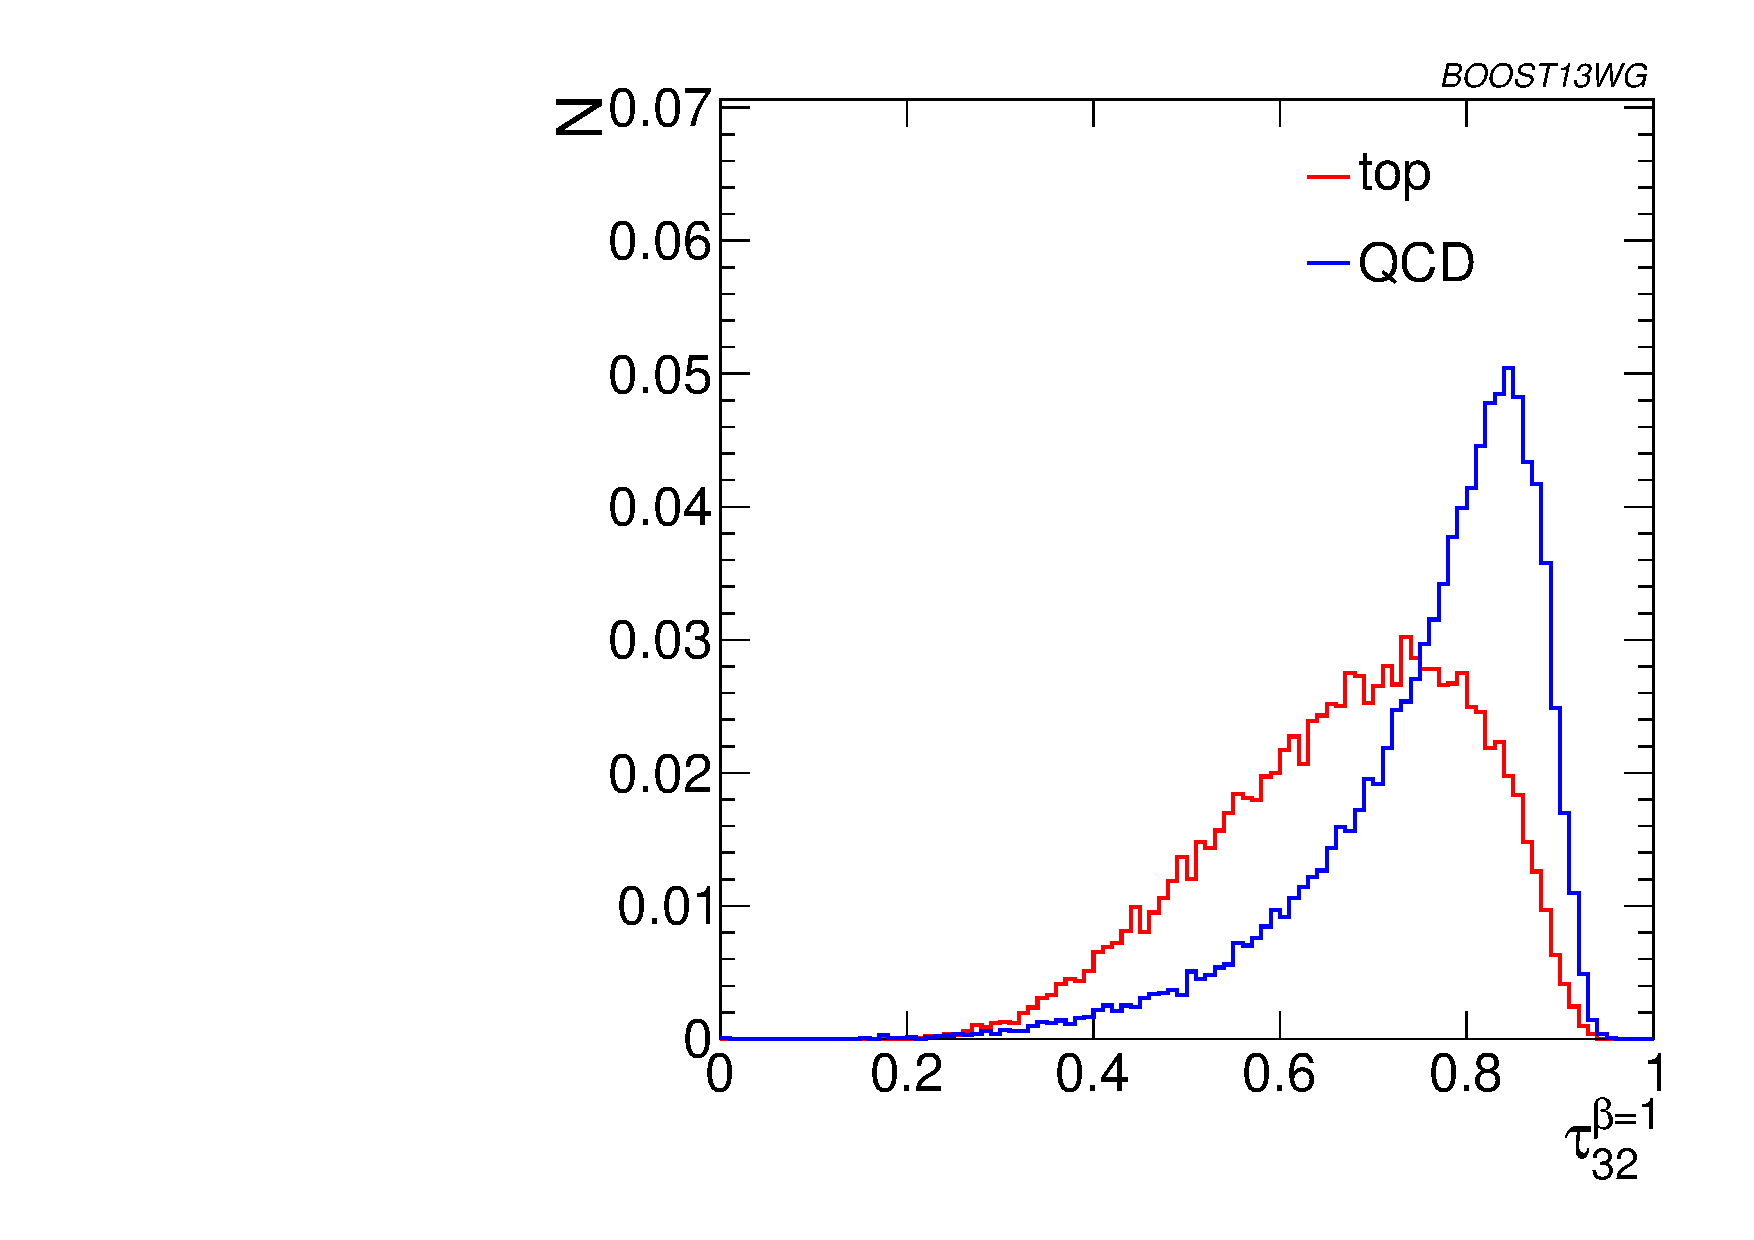
\includegraphics[width=0.245\textwidth]{./Figures/TTagging/single_variable/pT.1.5TeV.R.0.8/h_tau32b1_R_0_8.pdf}}
\caption{Comparison of $\Gamma_{\rm Qjet}$ and $\tau_{32}^{\beta=1}$ at $R=0.8$ and different values of the \pt. These shape variables are the most sensitive to varying \pt.}
\label{fig:Qjet_comparison_pT}
\end{figure*}

In Figures~\ref{fig:Rcomparison_singleshape_top} and~\ref{fig:Rcomparison_singletopmass_top} we directly compare ROC curves for jet-shape variable performance and top-mass performance, respectively, for three different jet radii  within the \pt = 1.5-1.6 TeV bin. Again, the input parameters of the taggers, groomers and shape variables are separately optimized for each jet radius. We can see from these figures that most of the top-tagging variables, both shape and reconstructed top mass, perform best for smaller radius, as was generally observed in the case of $W$-tagging in Section~\ref{sec:wtagging}. This is likely because, at such high \pt, most of the radiation from the top quark is confined within $R=0.4$, and having a larger jet radius makes the variable more susceptible to contamination from the underlying event and other uncorrelated radiation. In Figure~\ref{fig:C_comparison_R}, we compare the individual top signal and QCD background distributions for each shape variable considered in the \pt = 1.5-1.6 TeV bin for the various jet radii. 
 In Figures~\ref{fig:C_comparison_R} (a) to (h) the distributions for both signal and background broaden with increasing $R$, degrading the discriminating power. 
For $C_2^{\beta=1}$ and $C_3^{\beta=1}$, the background distributions are shifted to larger values as well. 
For the variable $\Gamma_{\rm Qjet}$, as already discussed for increasing \pt (and in  Section~\ref{sec:wtagging}) the behavior with increasing $R$ is a bit
more complicated, with the QCD jets becoming less volatile and the signal jets more volatile, \textit{i.e.}, the two volatility distributions become more
similar as we move from Figure~\ref{fig:C_comparison_R} (i) to Figure~\ref{fig:C_comparison_R} (j).  So again 
the discriminating power decreases with increasing $R$. 
The main exception is   for $C_3^{\beta=1}$, which performs optimally at $R=0.8$; in this case, the signal and background coincidentally 
happen to have the same distribution around $R=0.4$, and so $R=0.8$ gives better discrimination.


\begin{figure*}
\centering
\subfigure[$C_2^{\beta=1}$]{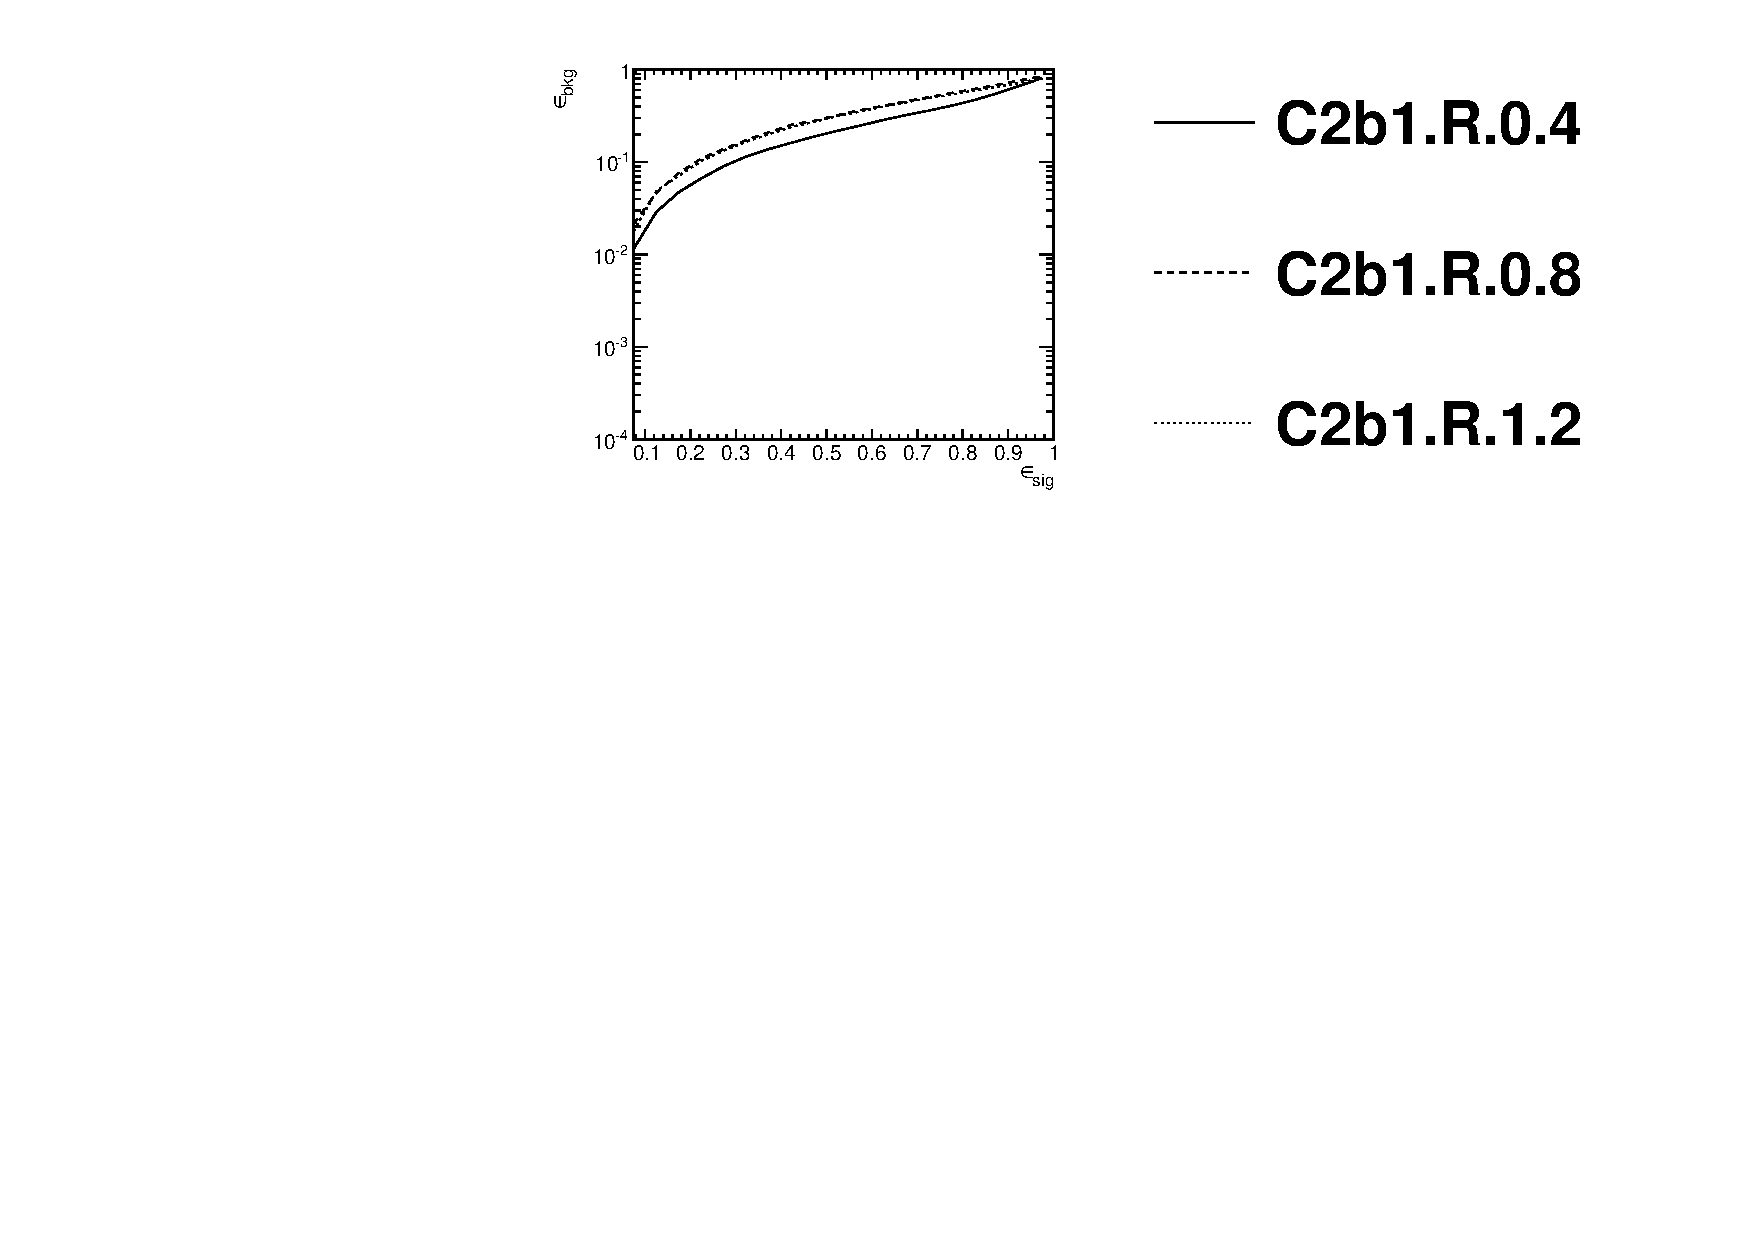
\includegraphics[width=0.48\textwidth]{./Figures/TTagging/single_variable/R_compare/Rocs_C2b1_Rcompare.pdf}}
\subfigure[$C_3^{\beta=1}$]{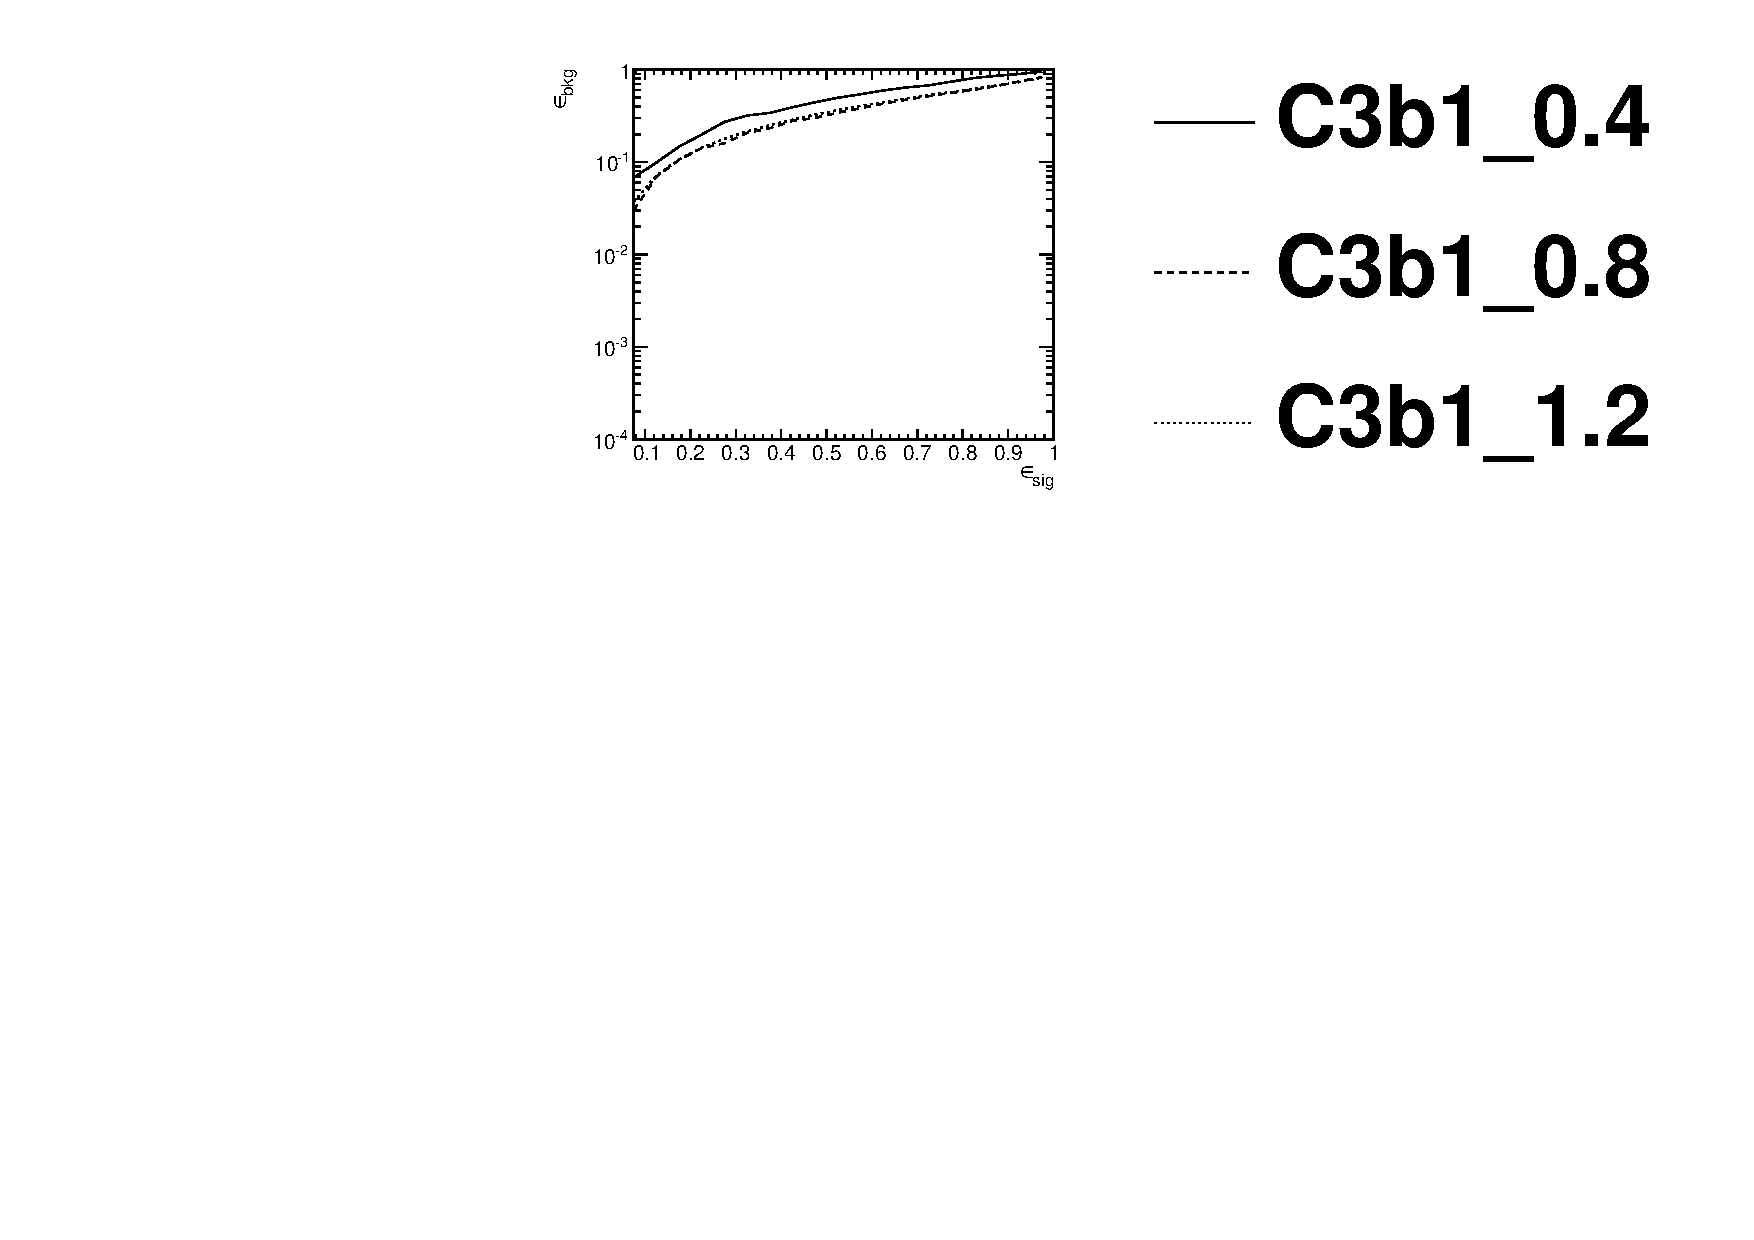
\includegraphics[width=0.48\textwidth]{./Figures/TTagging/single_variable/R_compare/Rocs_C3b1_Rcompare.pdf}}
\subfigure[\tautwoone]{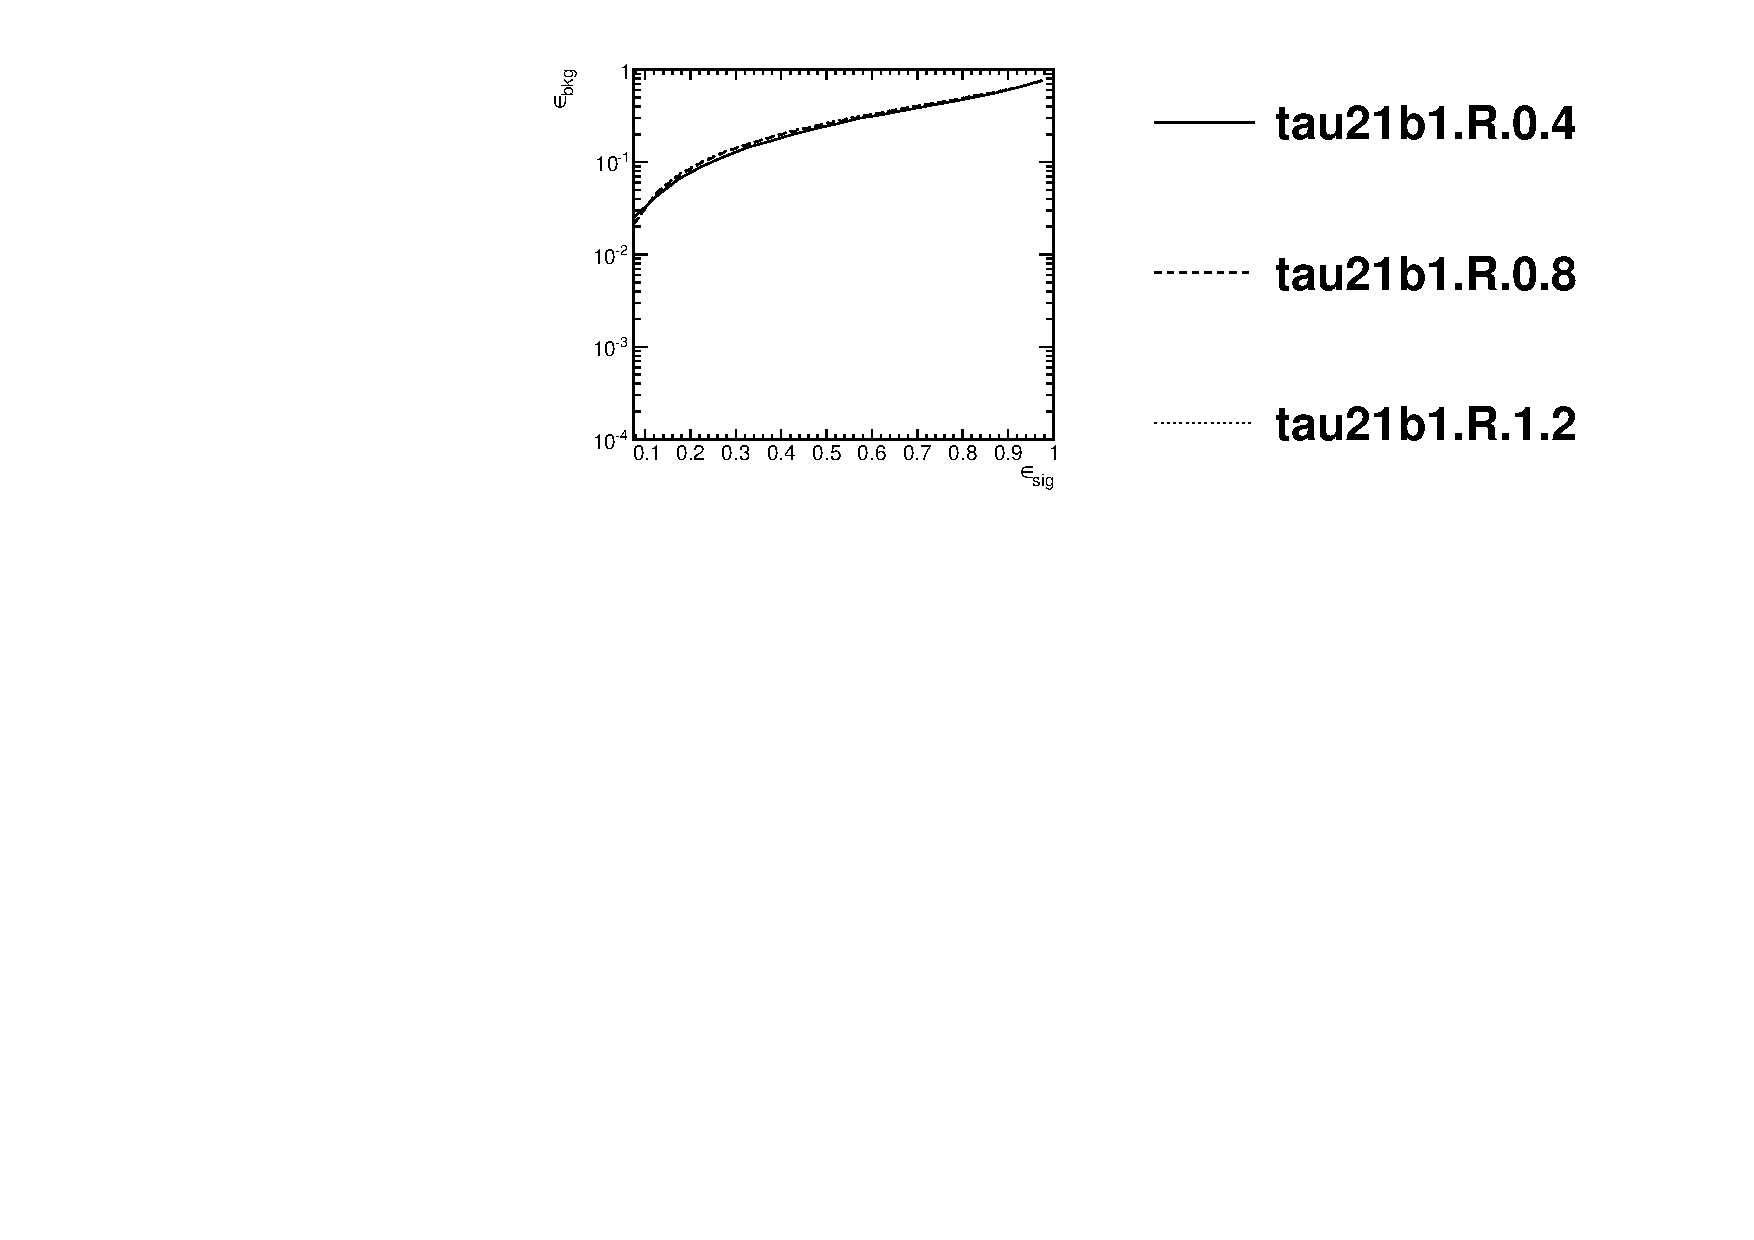
\includegraphics[width=0.48\textwidth]{./Figures/TTagging/single_variable/R_compare/Rocs_tau21b1_Rcompare.pdf}}
\subfigure[\tauthreetwo]{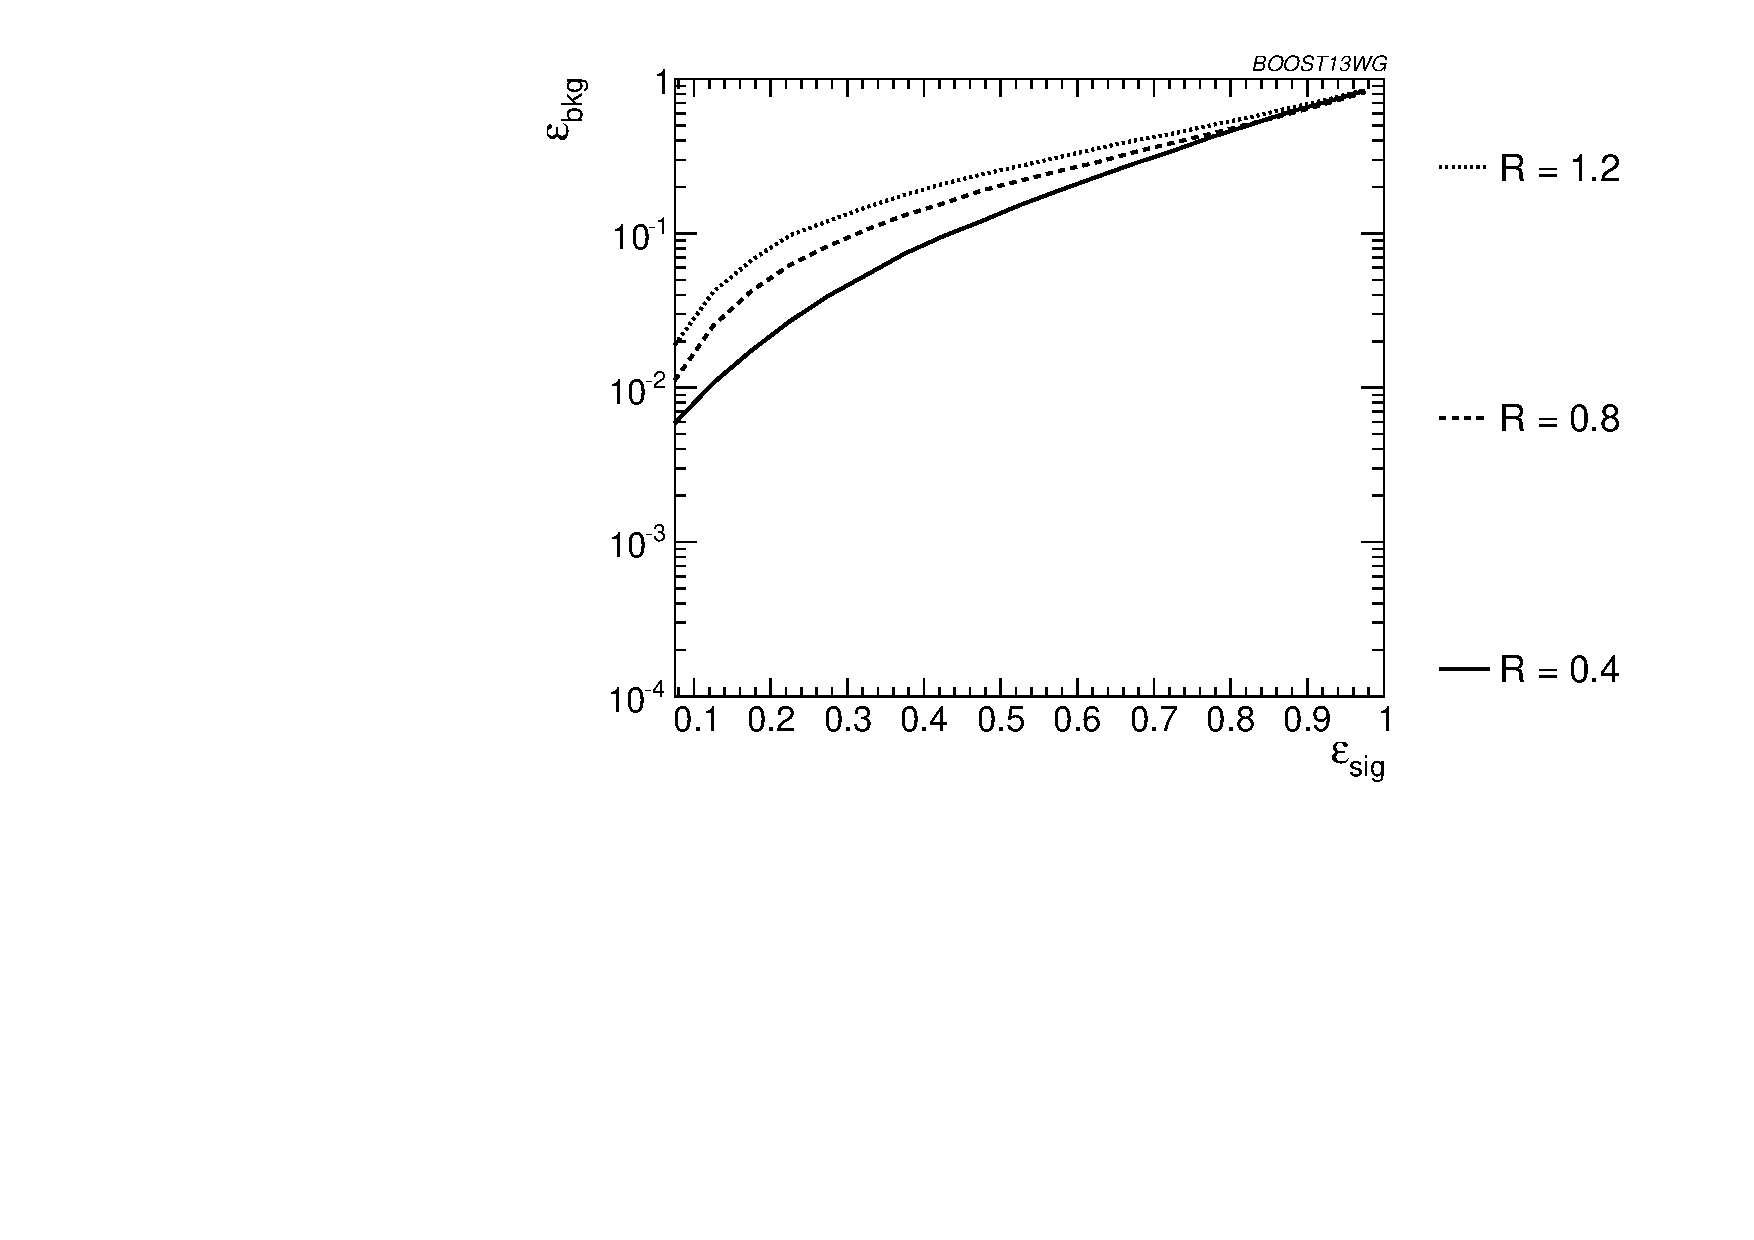
\includegraphics[width=0.48\textwidth]{./Figures/TTagging/single_variable/R_compare/Rocs_tau32b1_Rcompare.pdf}}
\subfigure[$\Gamma_{\rm Qjet}$]{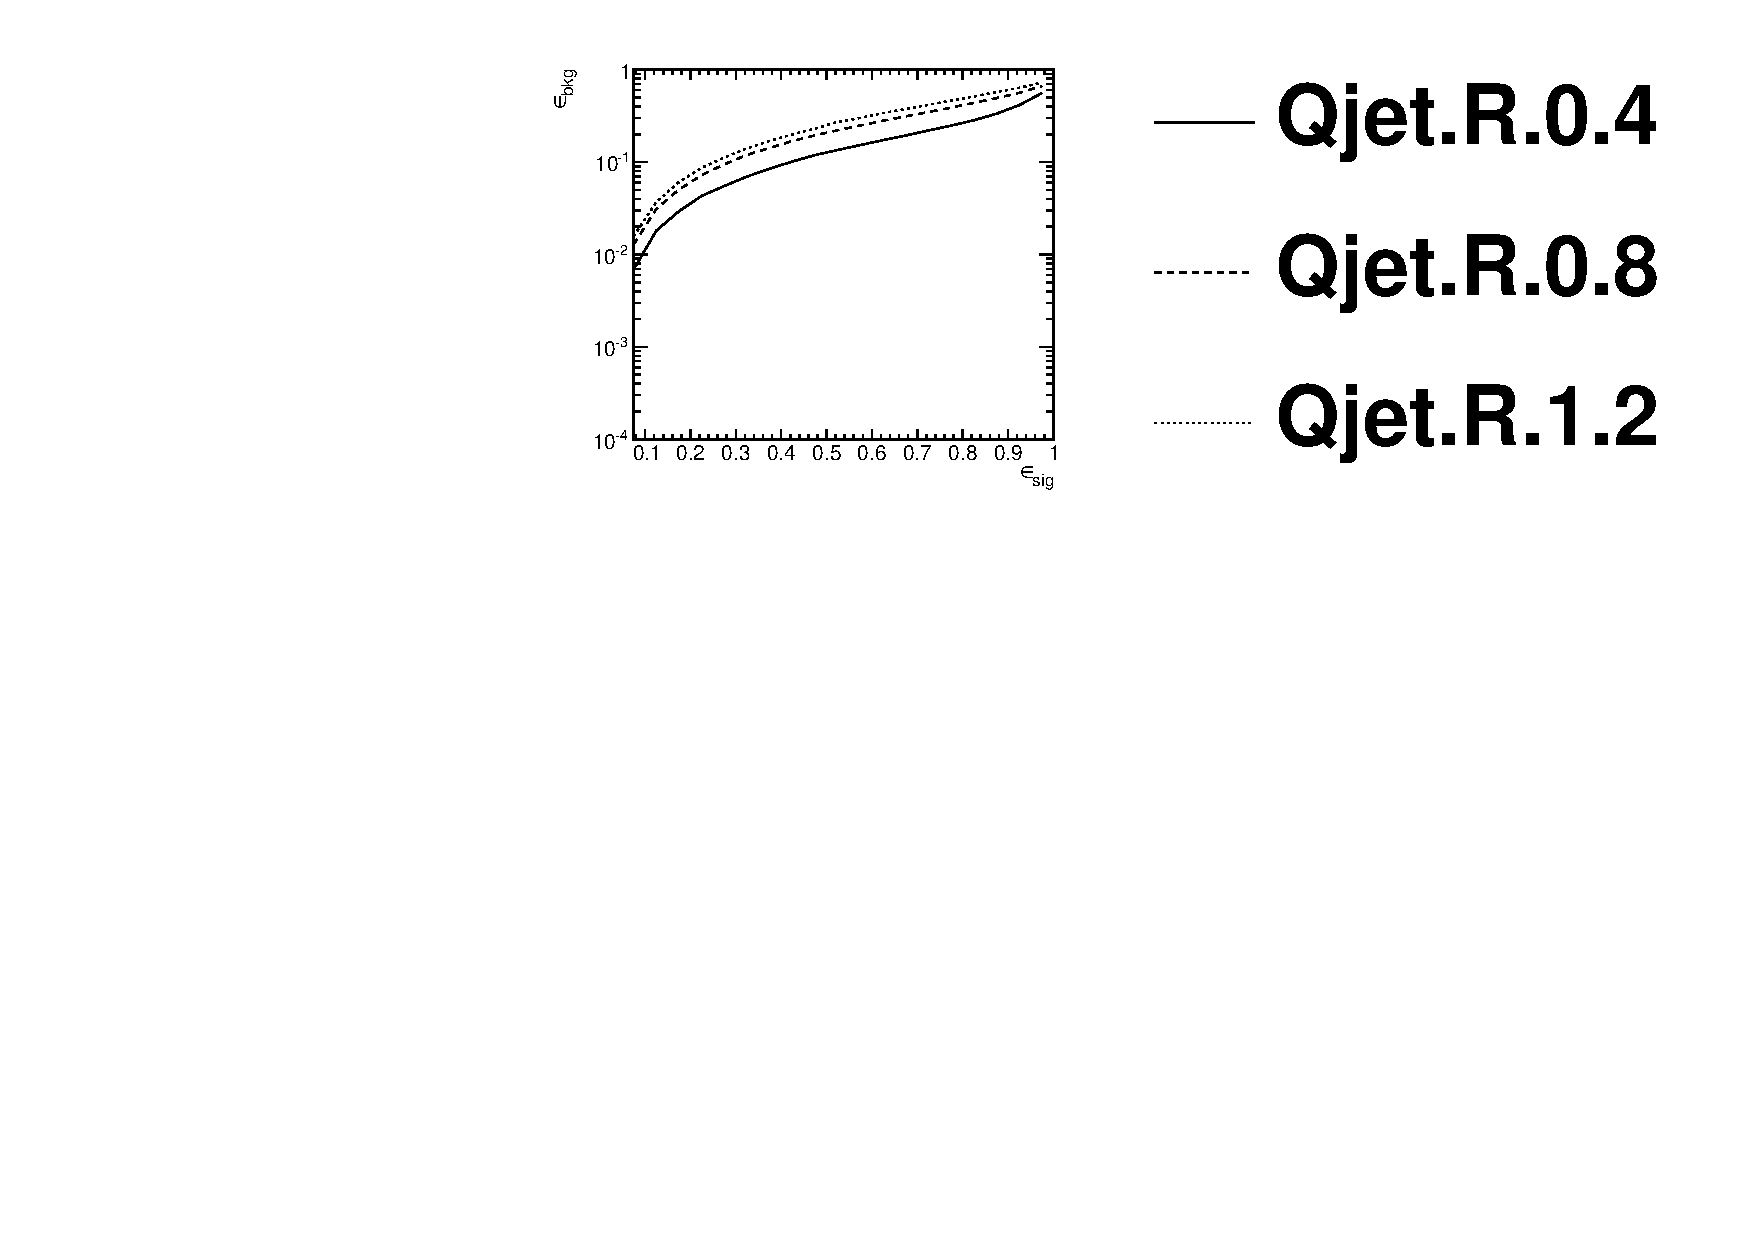
\includegraphics[width=0.48\textwidth]{./Figures/TTagging/single_variable/R_compare/Rocs_Qjet_Rcompare.pdf}}
\caption{Comparison of individual jet shape performance at different $R$ in the \pt = 1.5-1.6 \TeV bin.}
\label{fig:Rcomparison_singleshape_top}
\end{figure*}





\begin{figure*}
\centering
\subfigure[HEPTopTagger $m_t$]{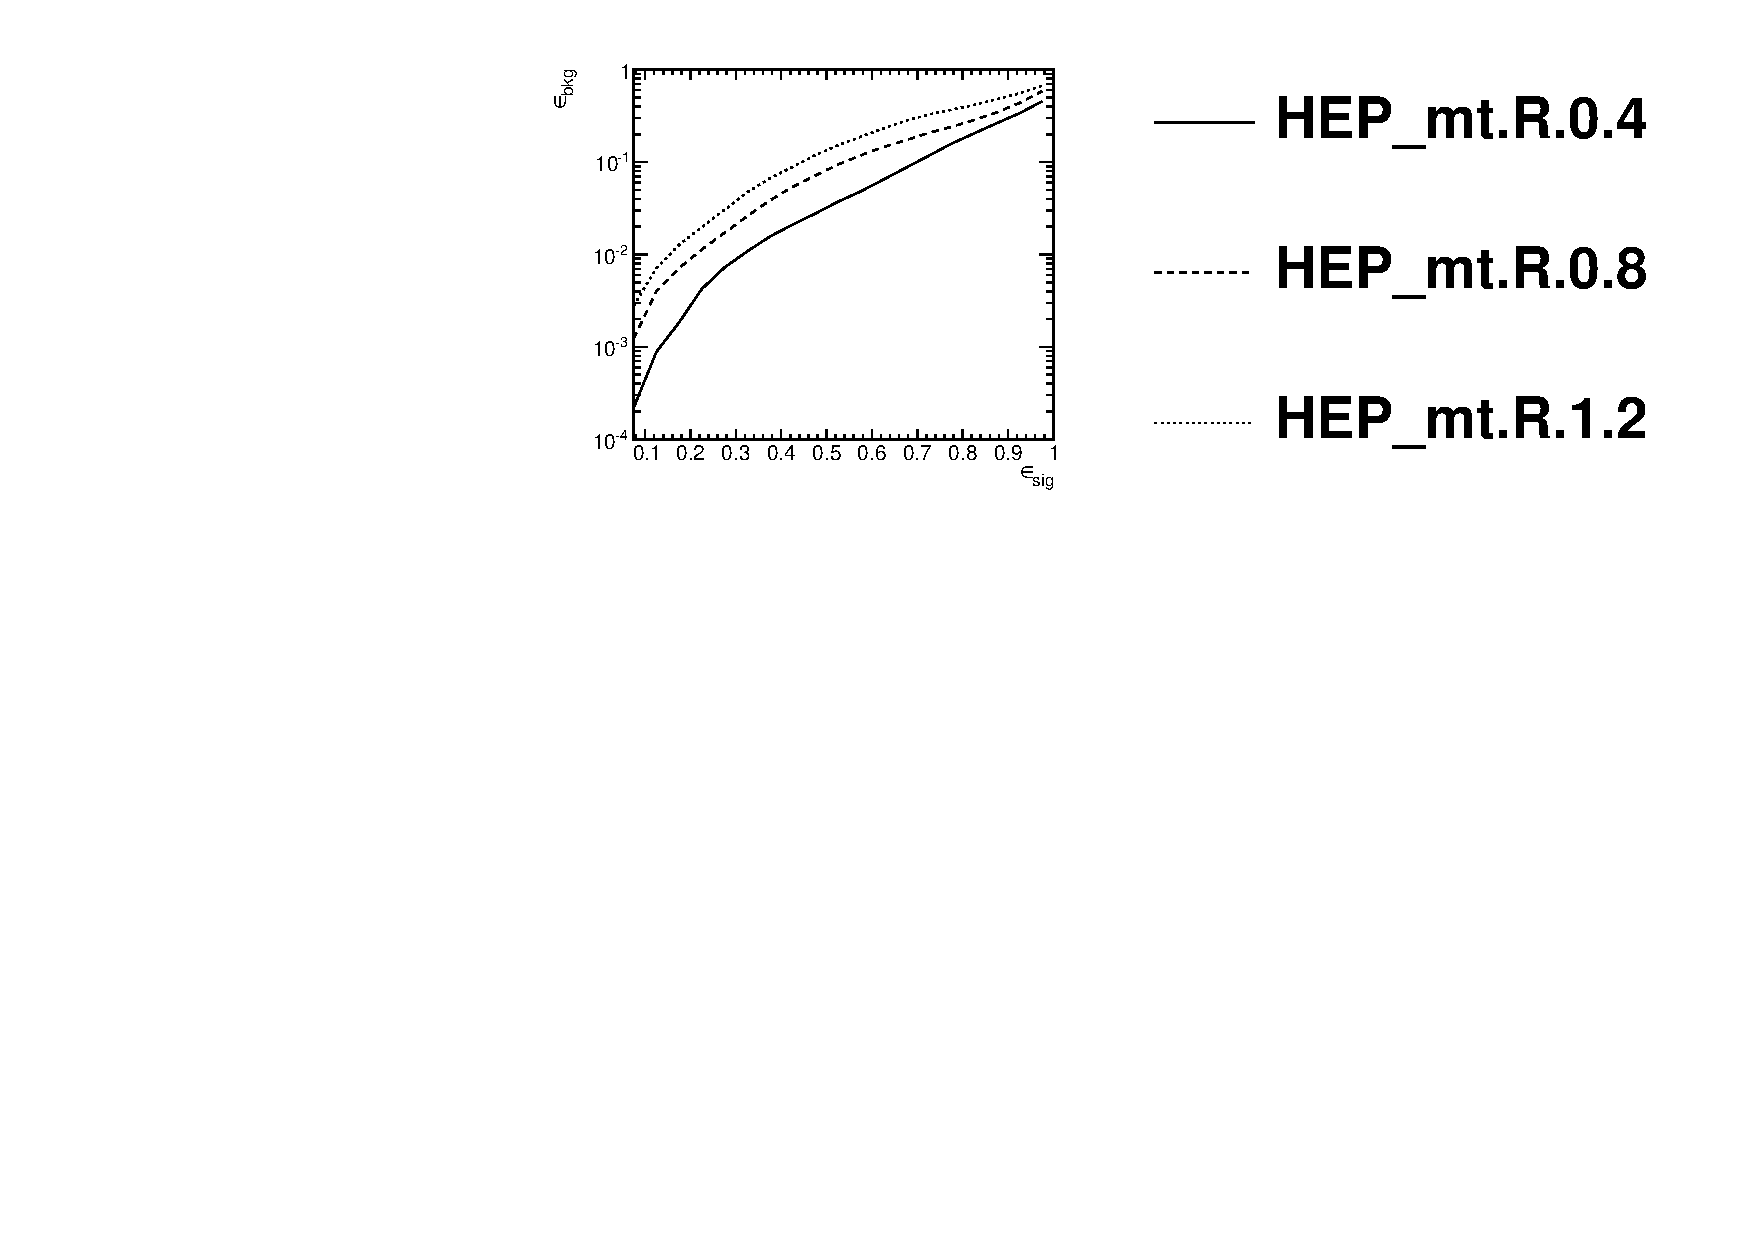
\includegraphics[width=0.48\textwidth]{./Figures/TTagging/single_variable/R_compare/Rocs_HEP_mt_Rcompare.pdf}}
\subfigure[Johns Hopkins Tagger $m_t$]{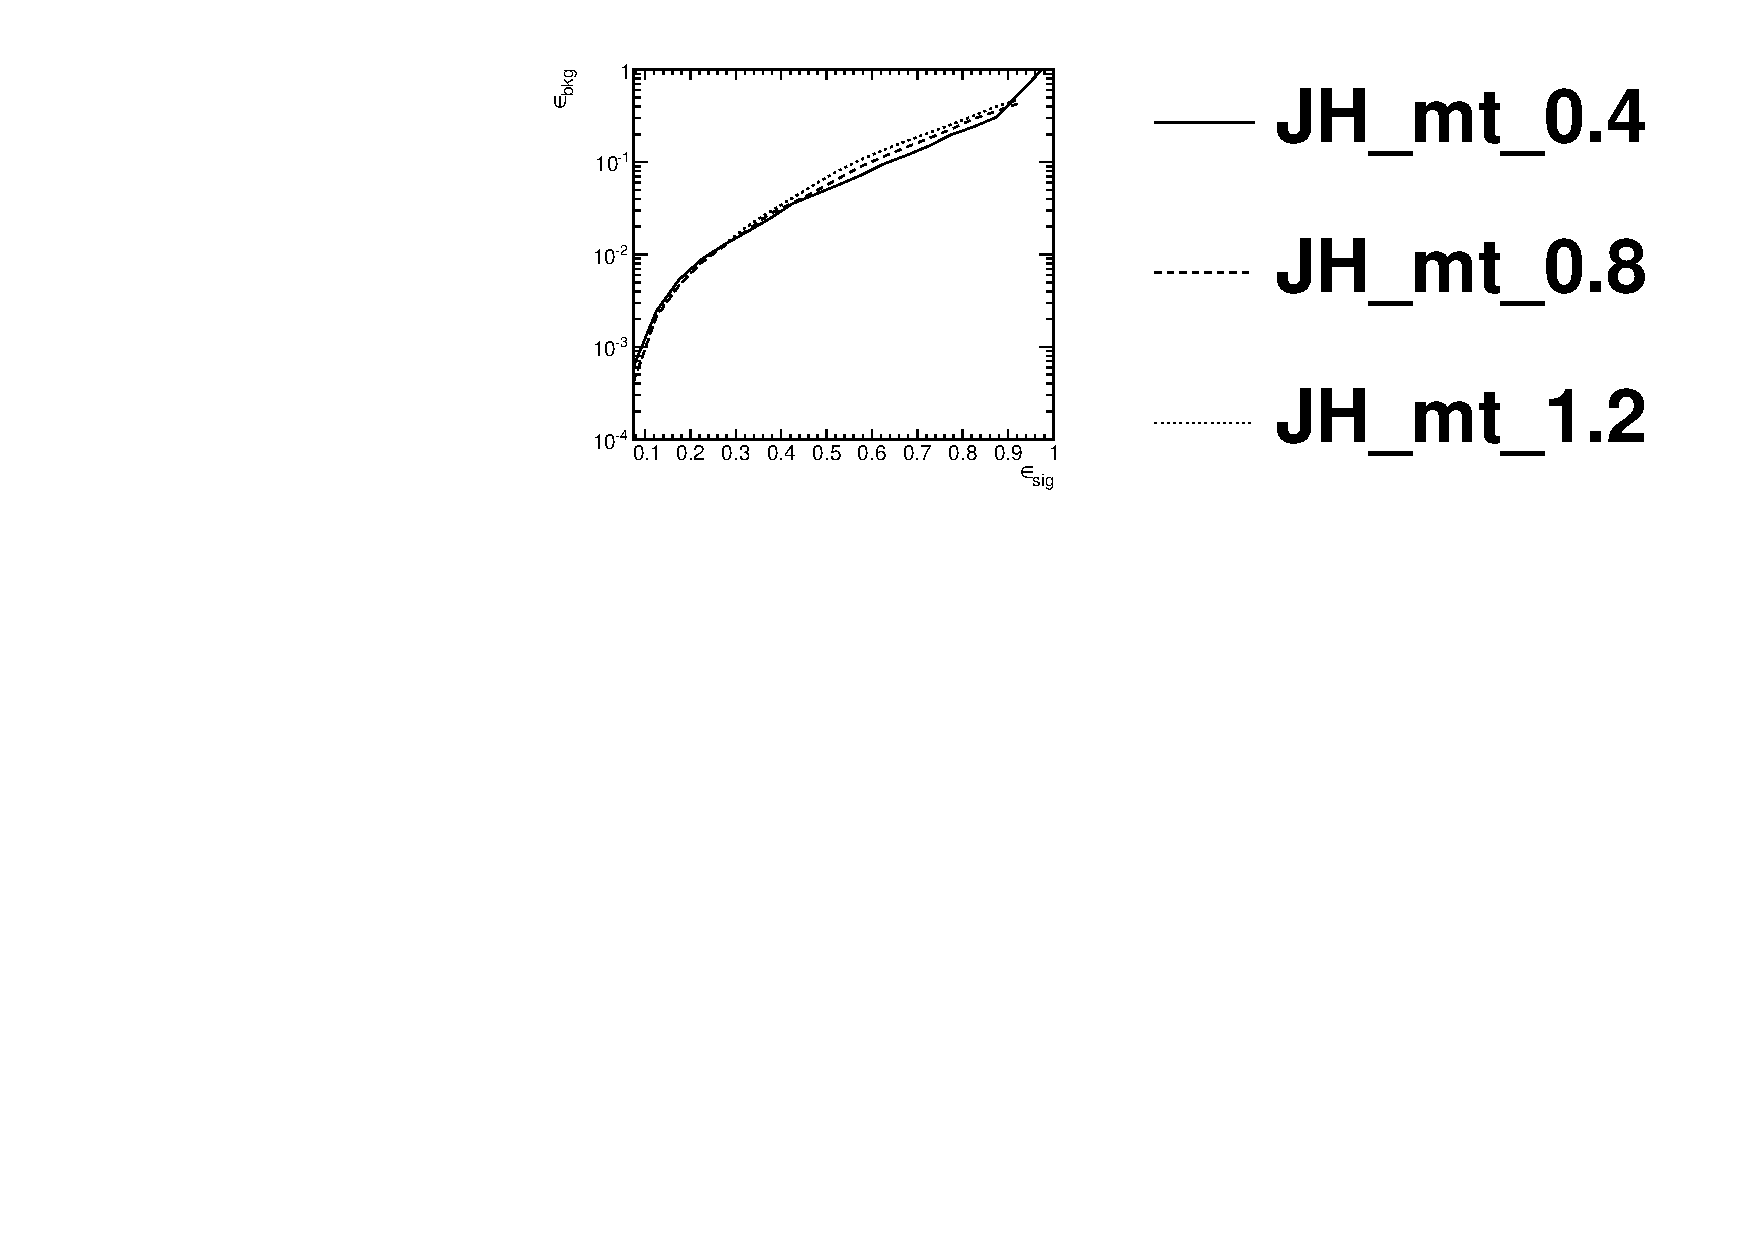
\includegraphics[width=0.48\textwidth]{./Figures/TTagging/single_variable/R_compare/Rocs_JH_mt_Rcompare.pdf}}
\subfigure[Pruning $m_t$]{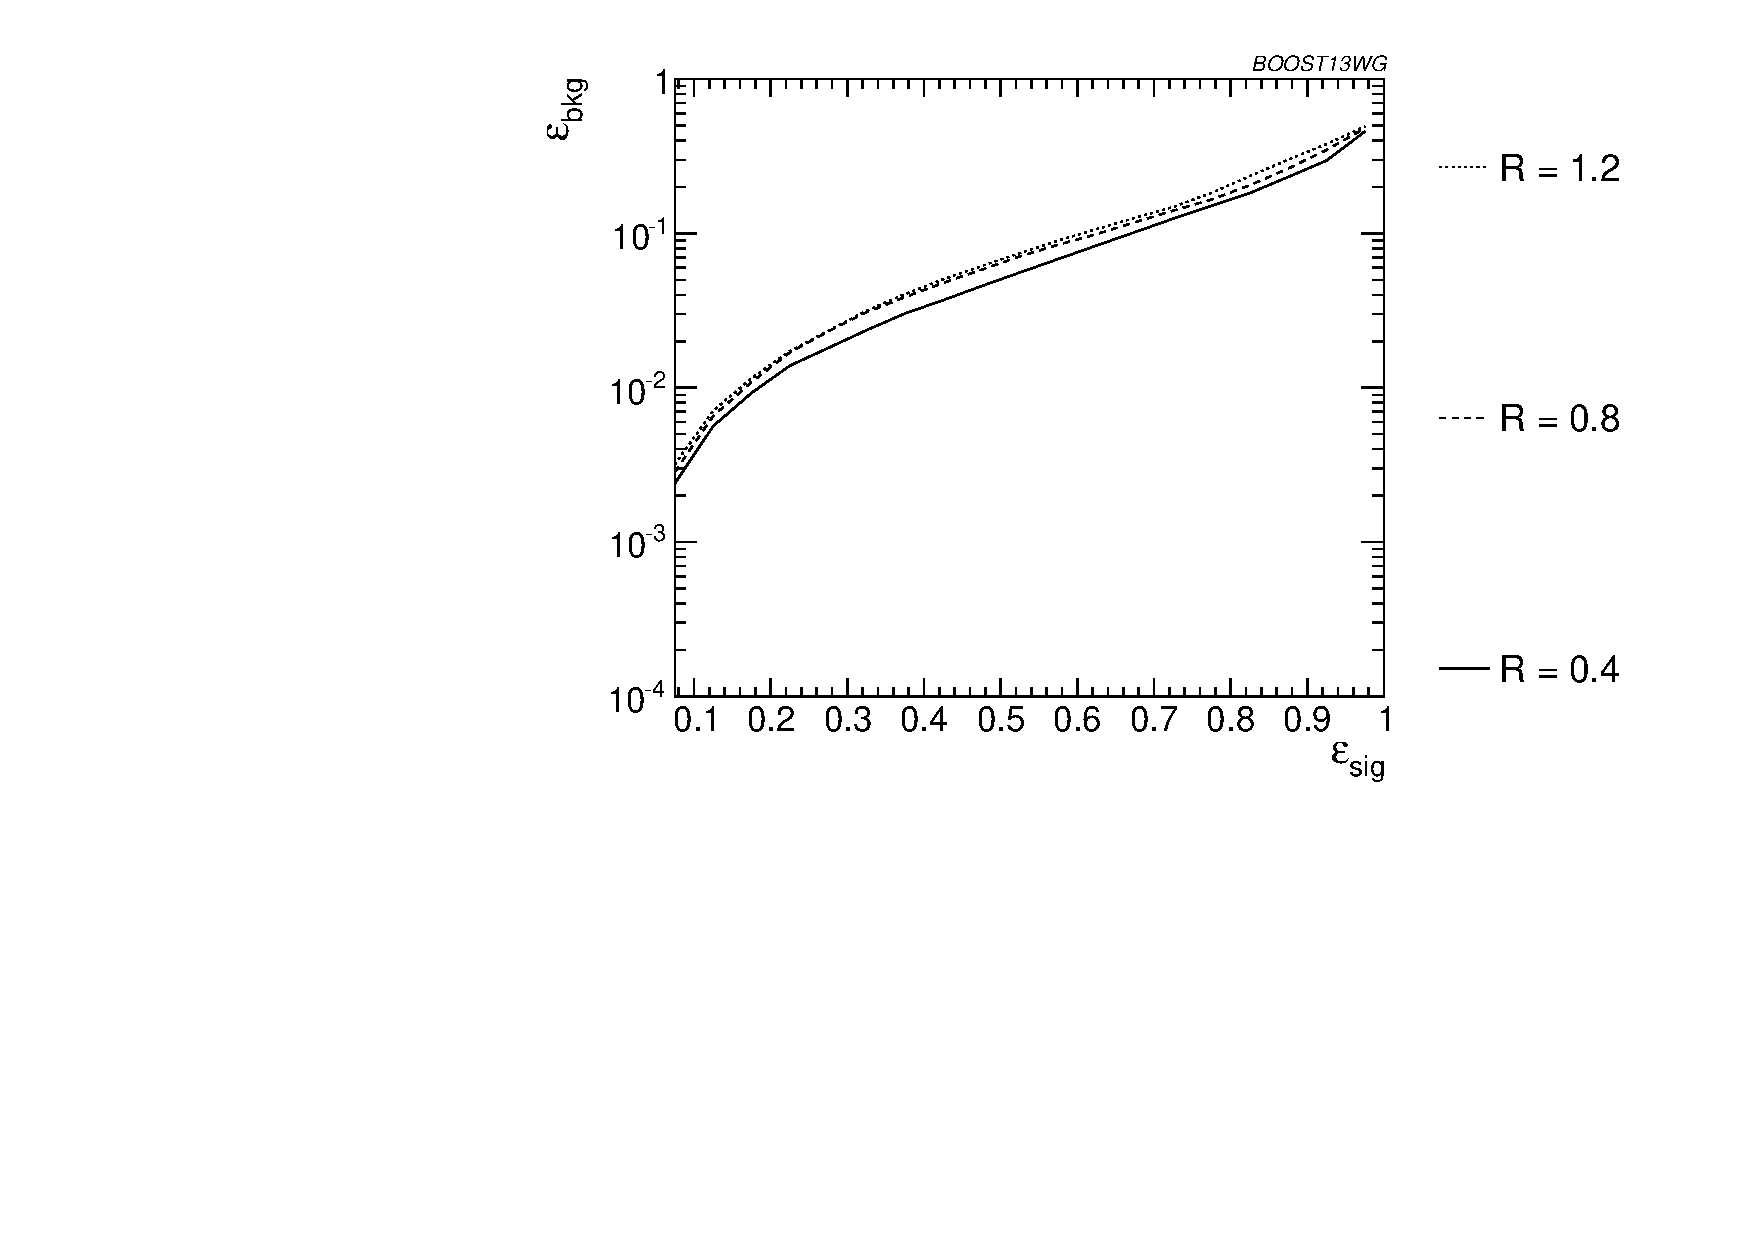
\includegraphics[width=0.48\textwidth]{./Figures/TTagging/single_variable/R_compare/Rocs_prune_Rcompare.pdf}}
\subfigure[Trimming $m_t$]{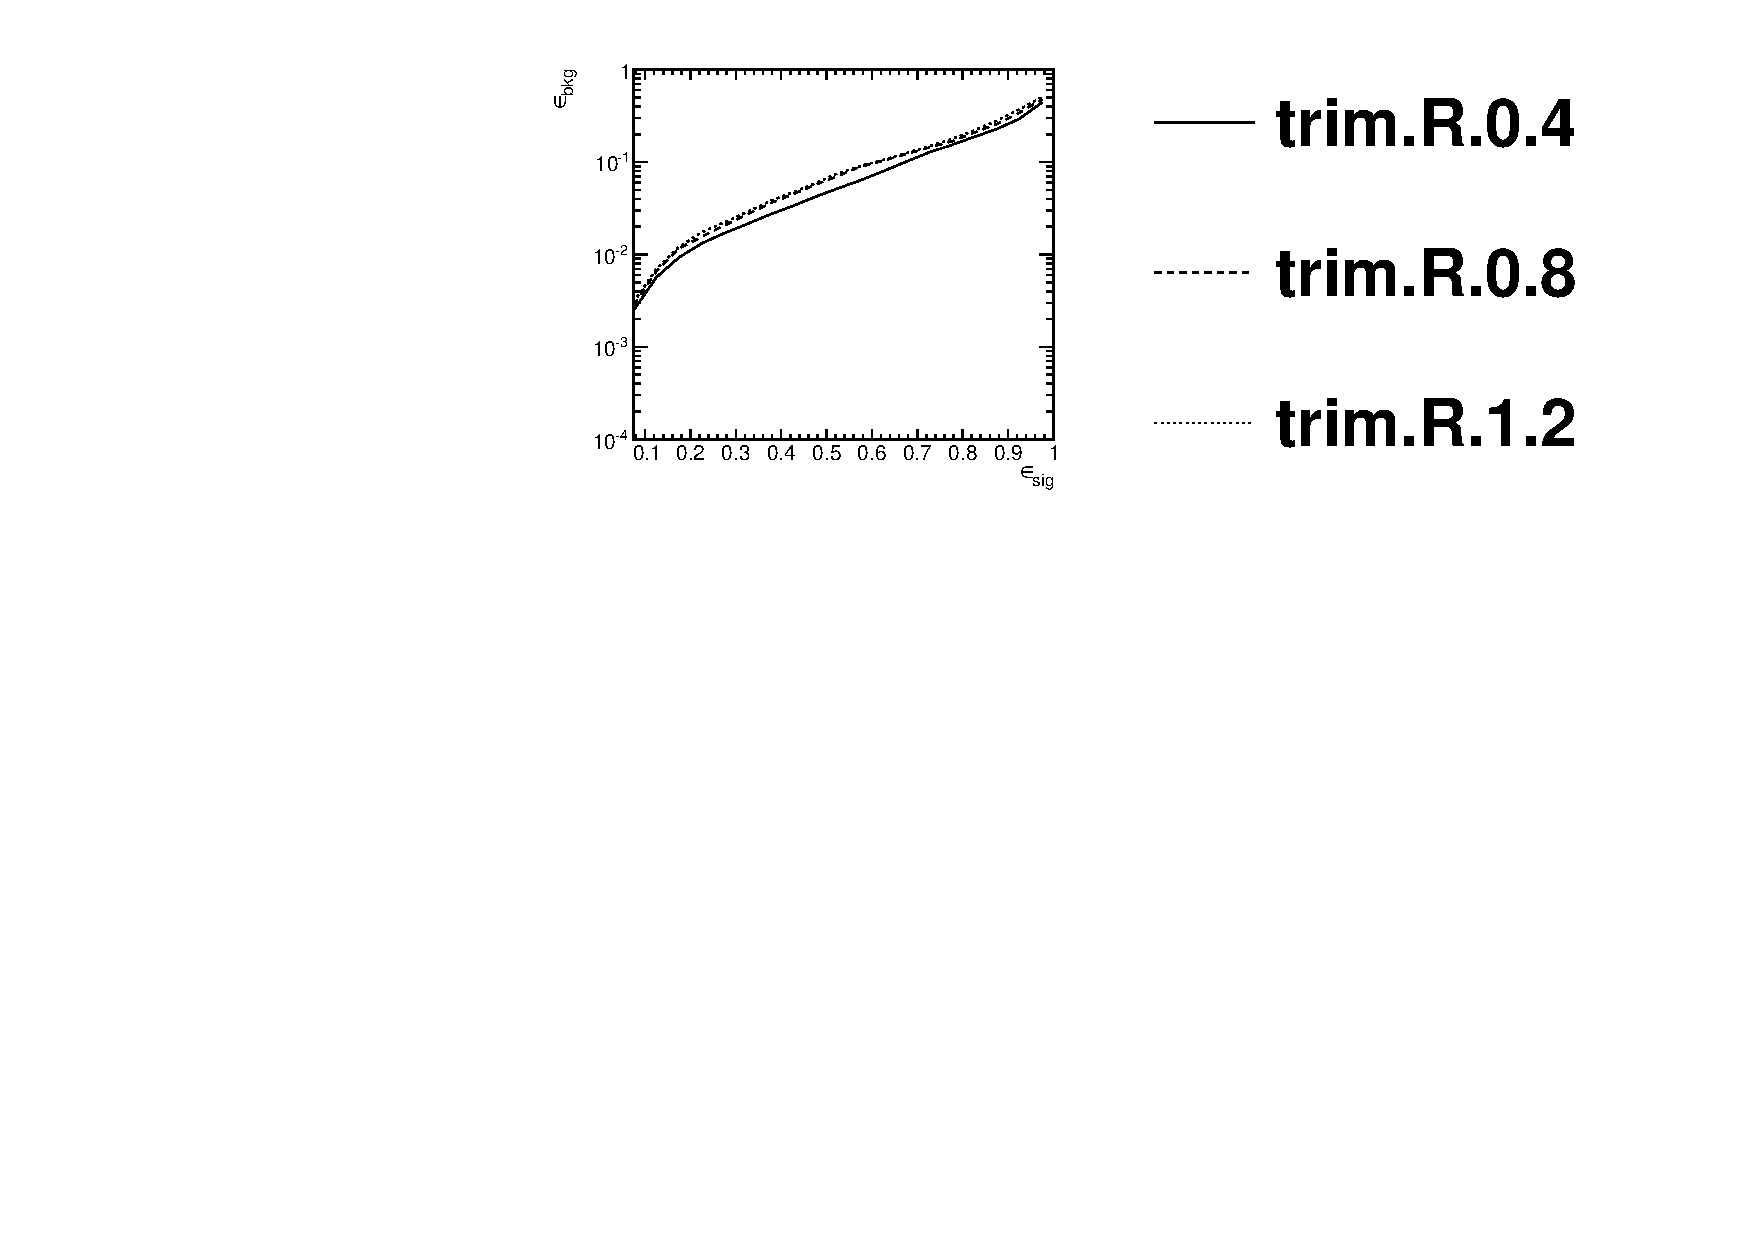
\includegraphics[width=0.48\textwidth]{./Figures/TTagging/single_variable/R_compare/Rocs_trim_Rcompare.pdf}}
\caption{Comparison of top mass performance of different taggers at different $R$ in the \pt = 1.5-1.6 \TeV bin.}
\label{fig:Rcomparison_singletopmass_top}
\end{figure*}

\begin{figure*}
\centering
\subfigure[$C_2^{\beta=1}$, $R=0.4$]{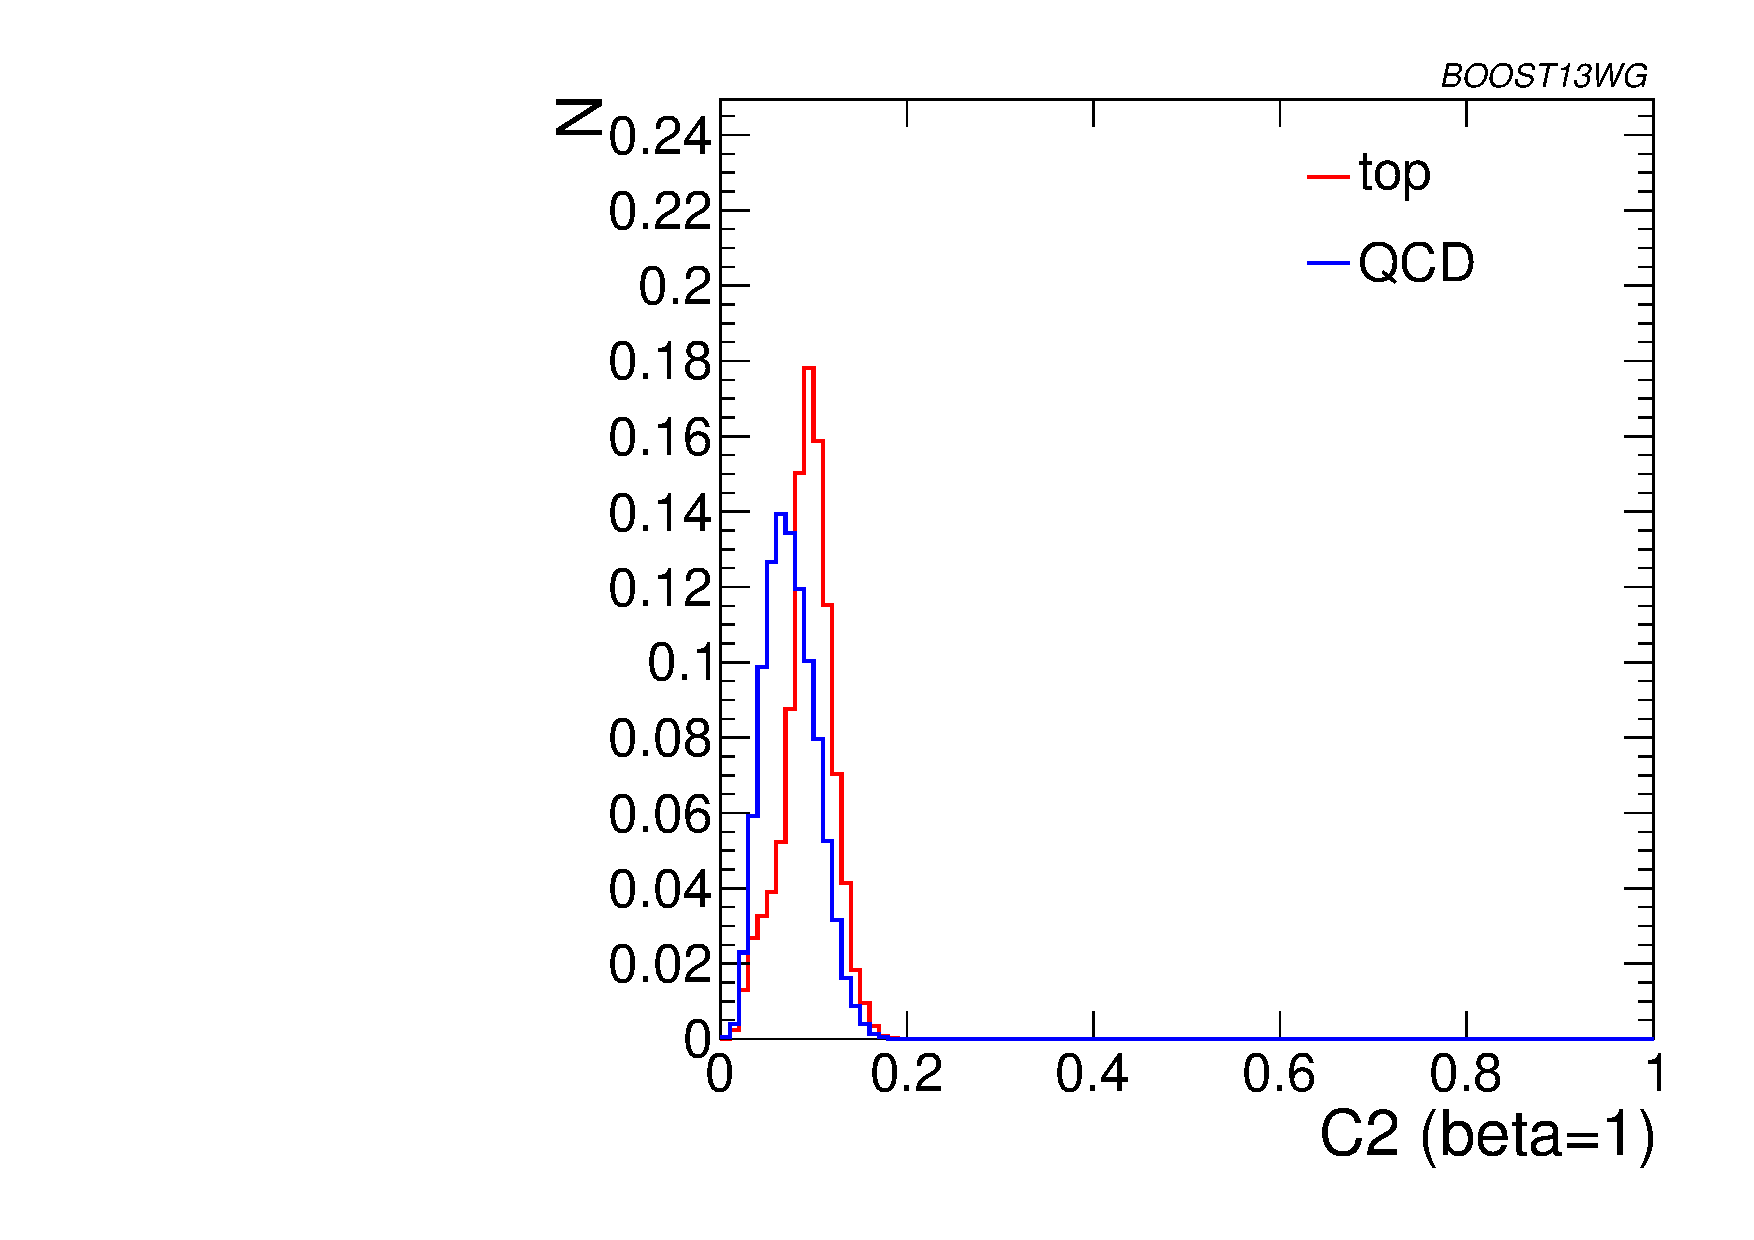
\includegraphics[width=0.245\textwidth]{./Figures/TTagging/single_variable/pT.1.5TeV.R.0.4/h_C2B1_R_0_4.pdf}}
\subfigure[$C_2^{\beta=1}$, $R=1.2$]{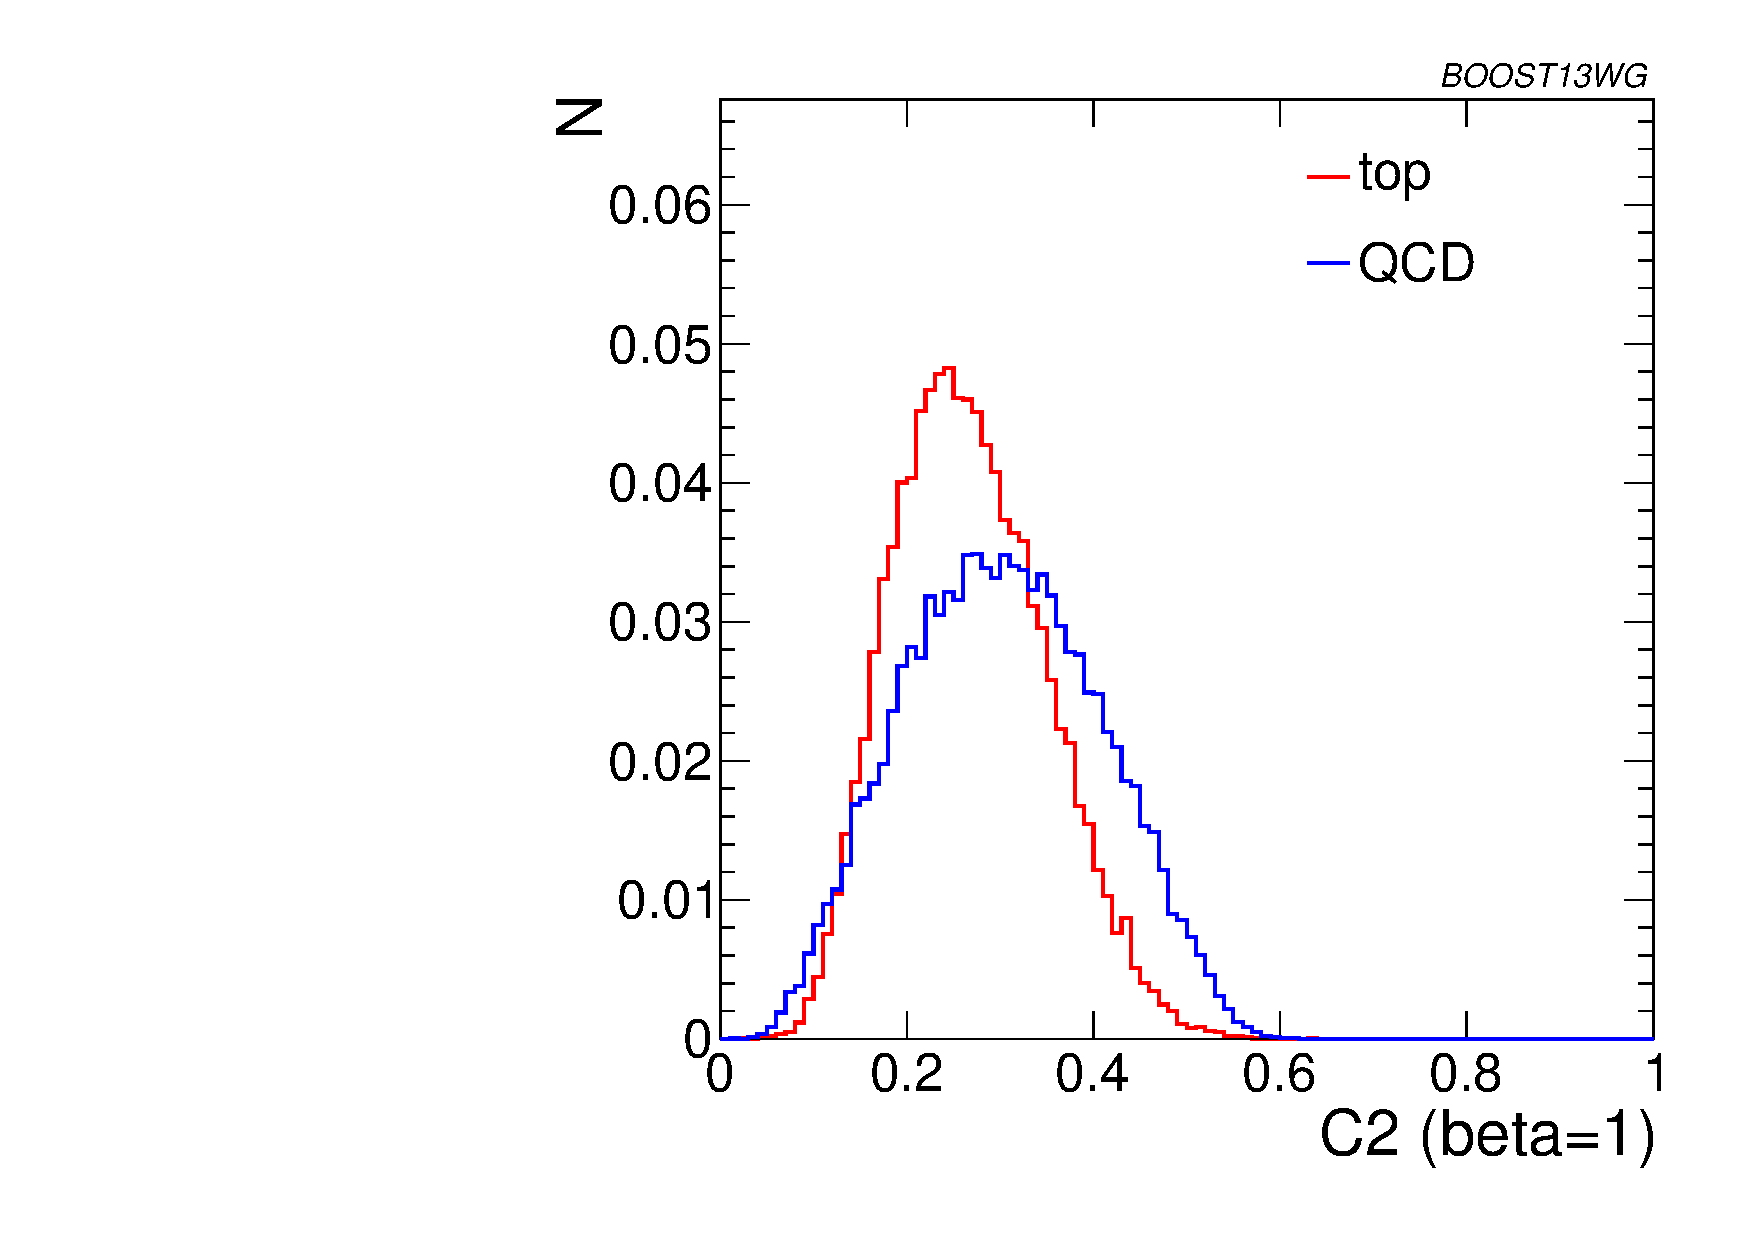
\includegraphics[width=0.245\textwidth]{./Figures/TTagging/single_variable/pT.1.5TeV.R.1.2/h_C2B1_R_1_2.pdf}}
\subfigure[$C_3^{\beta=1}$, $R=0.4$]{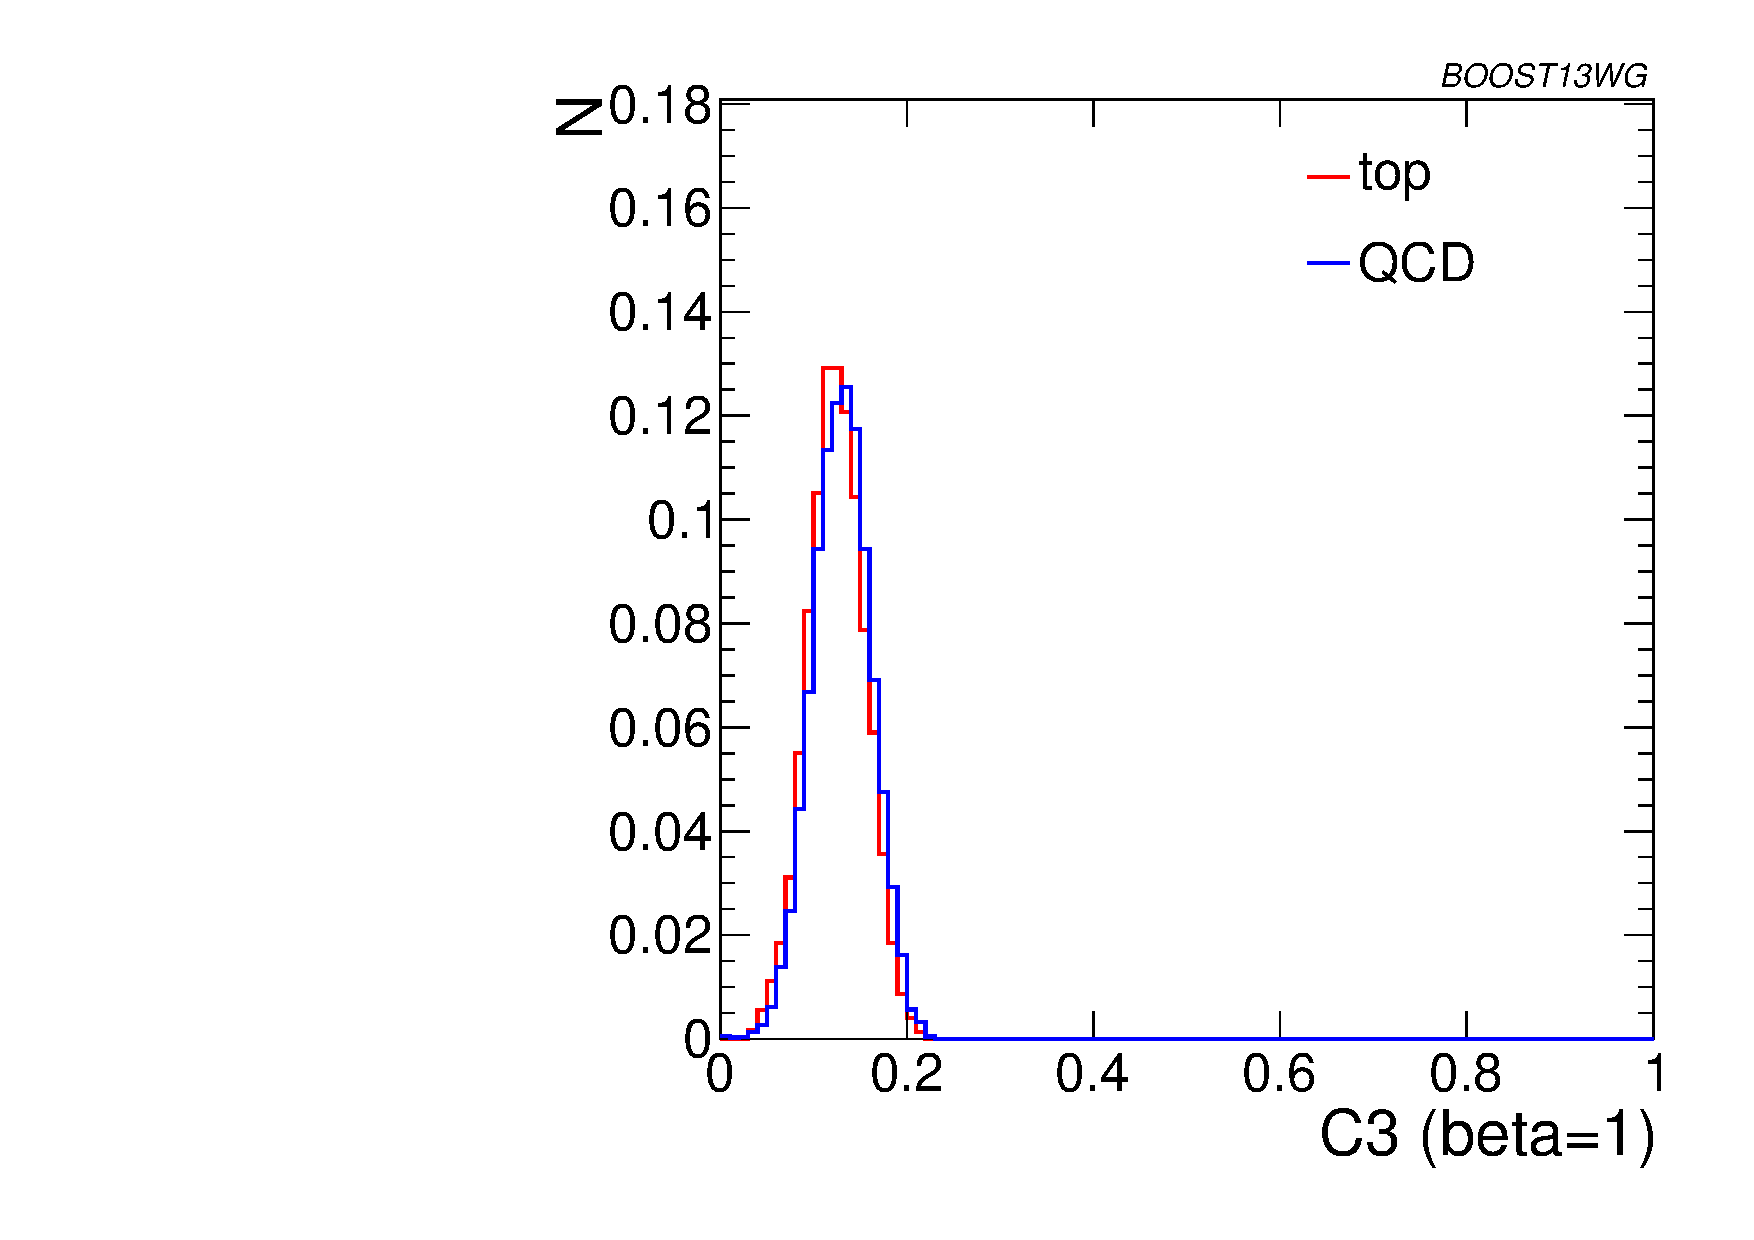
\includegraphics[width=0.245\textwidth]{./Figures/TTagging/single_variable/pT.1.5TeV.R.0.4/h_C3B1_R_0_4.pdf}}
\subfigure[$C_3^{\beta=1}$, $R=1.2$]{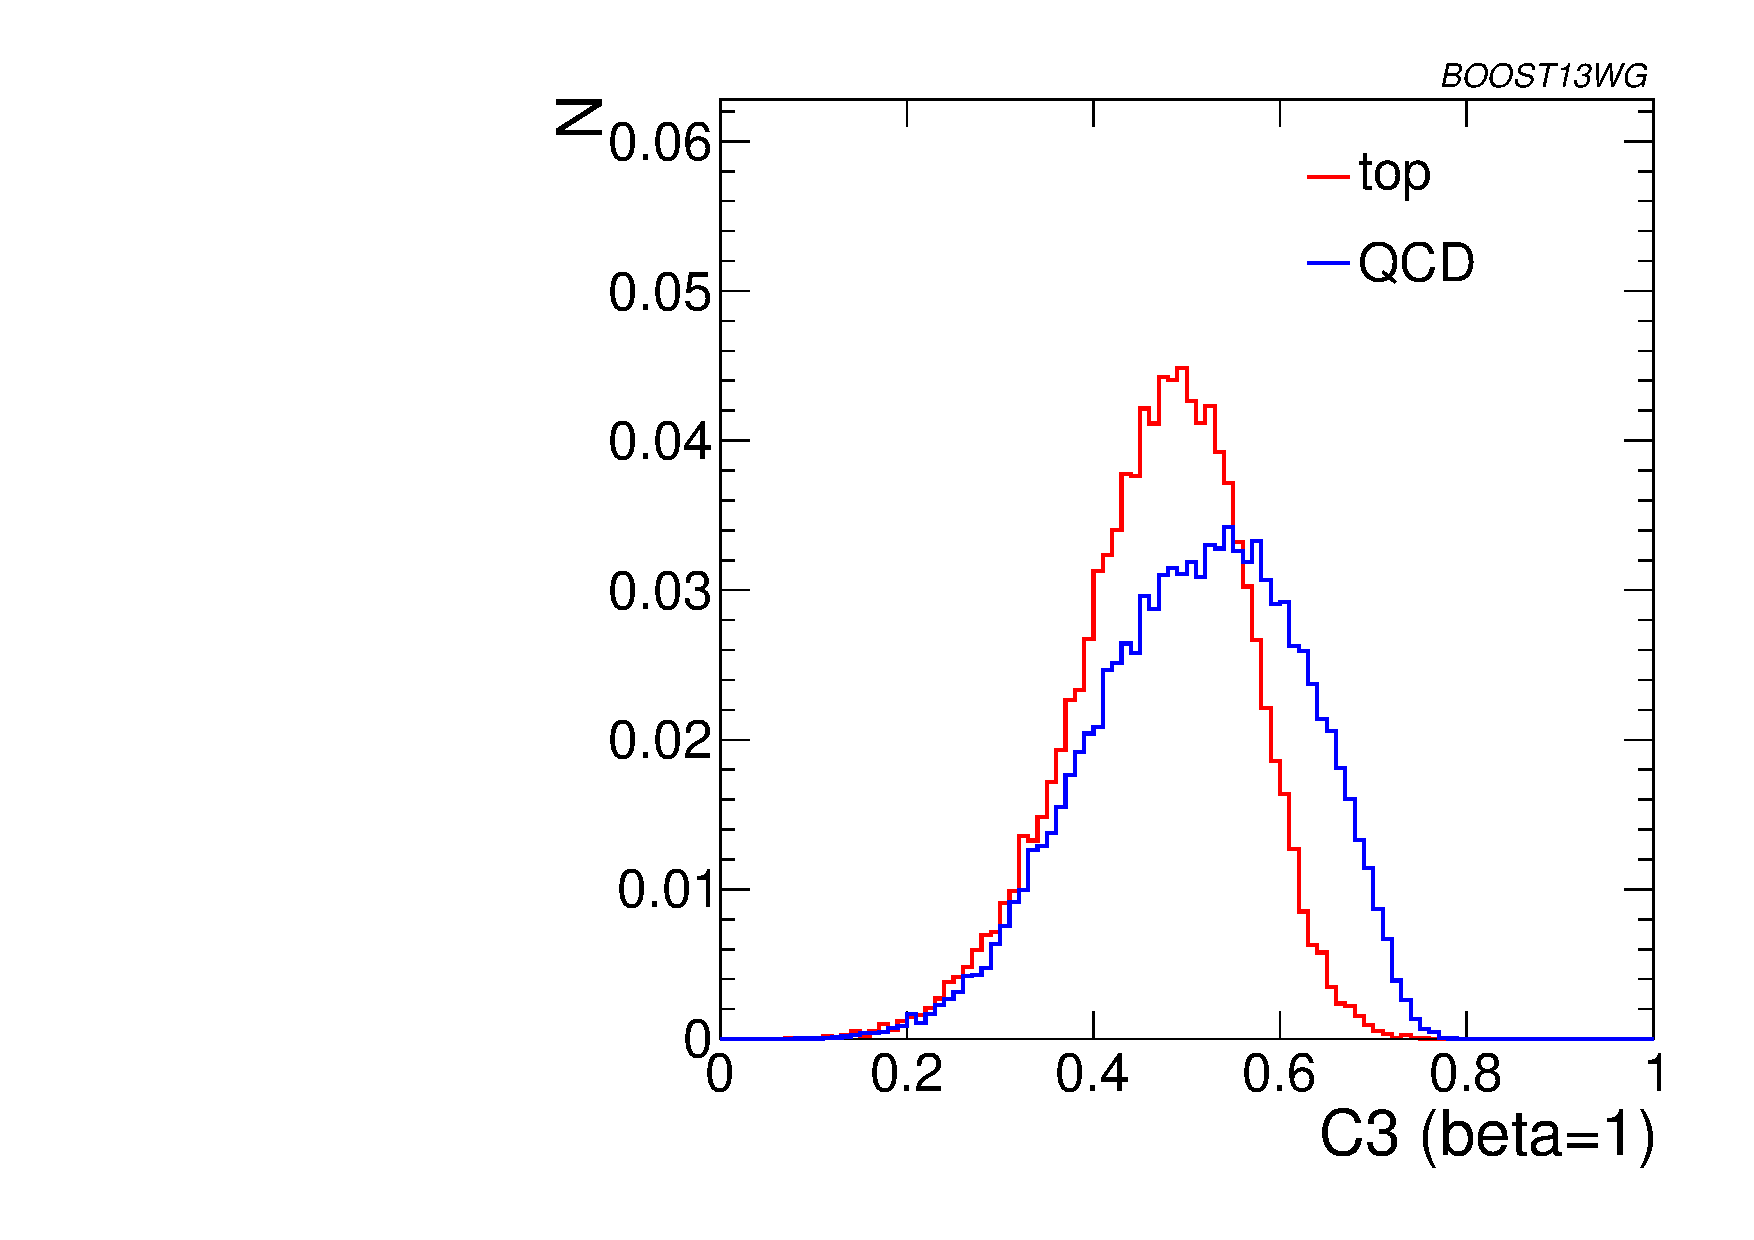
\includegraphics[width=0.245\textwidth]{./Figures/TTagging/single_variable/pT.1.5TeV.R.1.2/h_C3B1_R_1_2.pdf}}\\
\subfigure[\tautwoone, $R=0.4$]{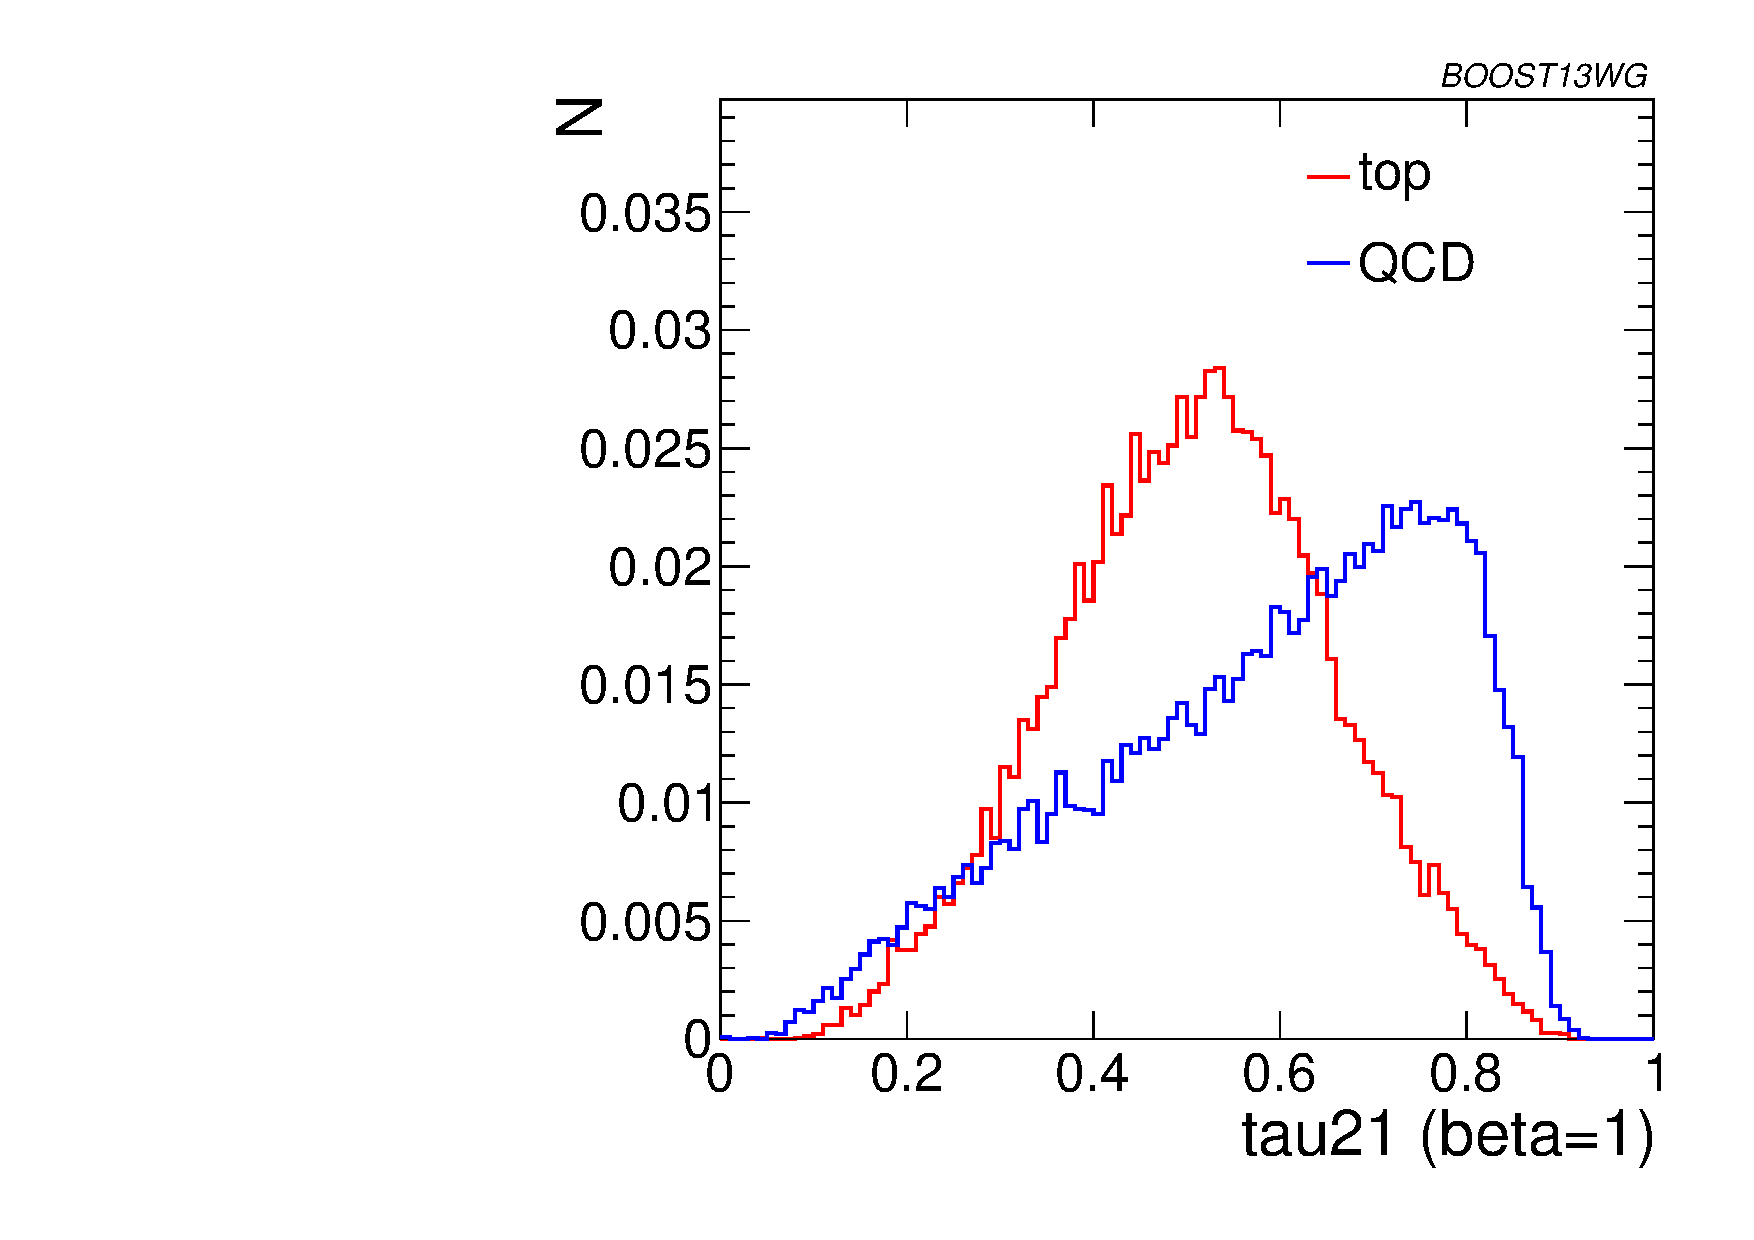
\includegraphics[width=0.245\textwidth]{./Figures/TTagging/single_variable/pT.1.5TeV.R.0.4/h_tau21b1_R_0_4.pdf}}
\subfigure[\tautwoone, $R=1.2$]{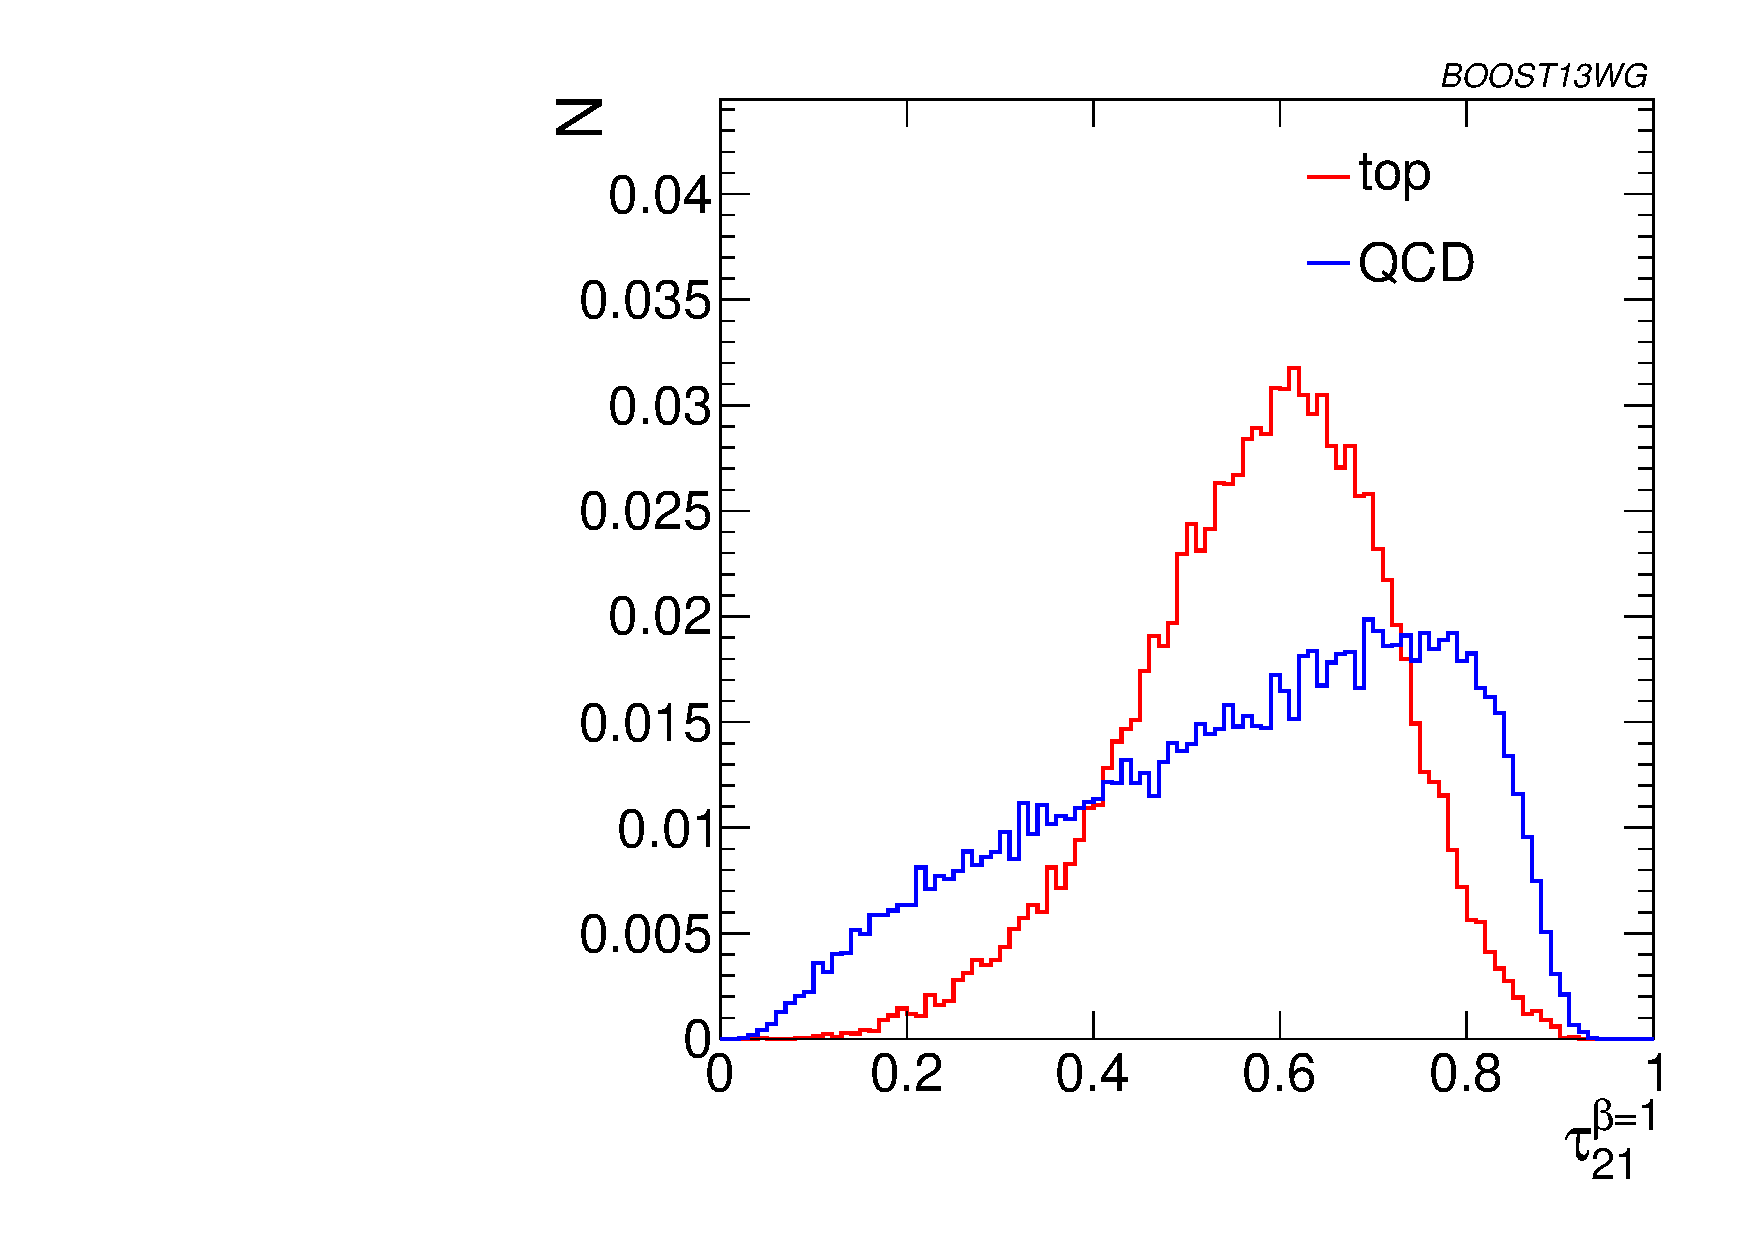
\includegraphics[width=0.245\textwidth]{./Figures/TTagging/single_variable/pT.1.5TeV.R.1.2/h_tau21b1_R_1_2.pdf}}
\subfigure[\tauthreetwo, $R=0.4$]{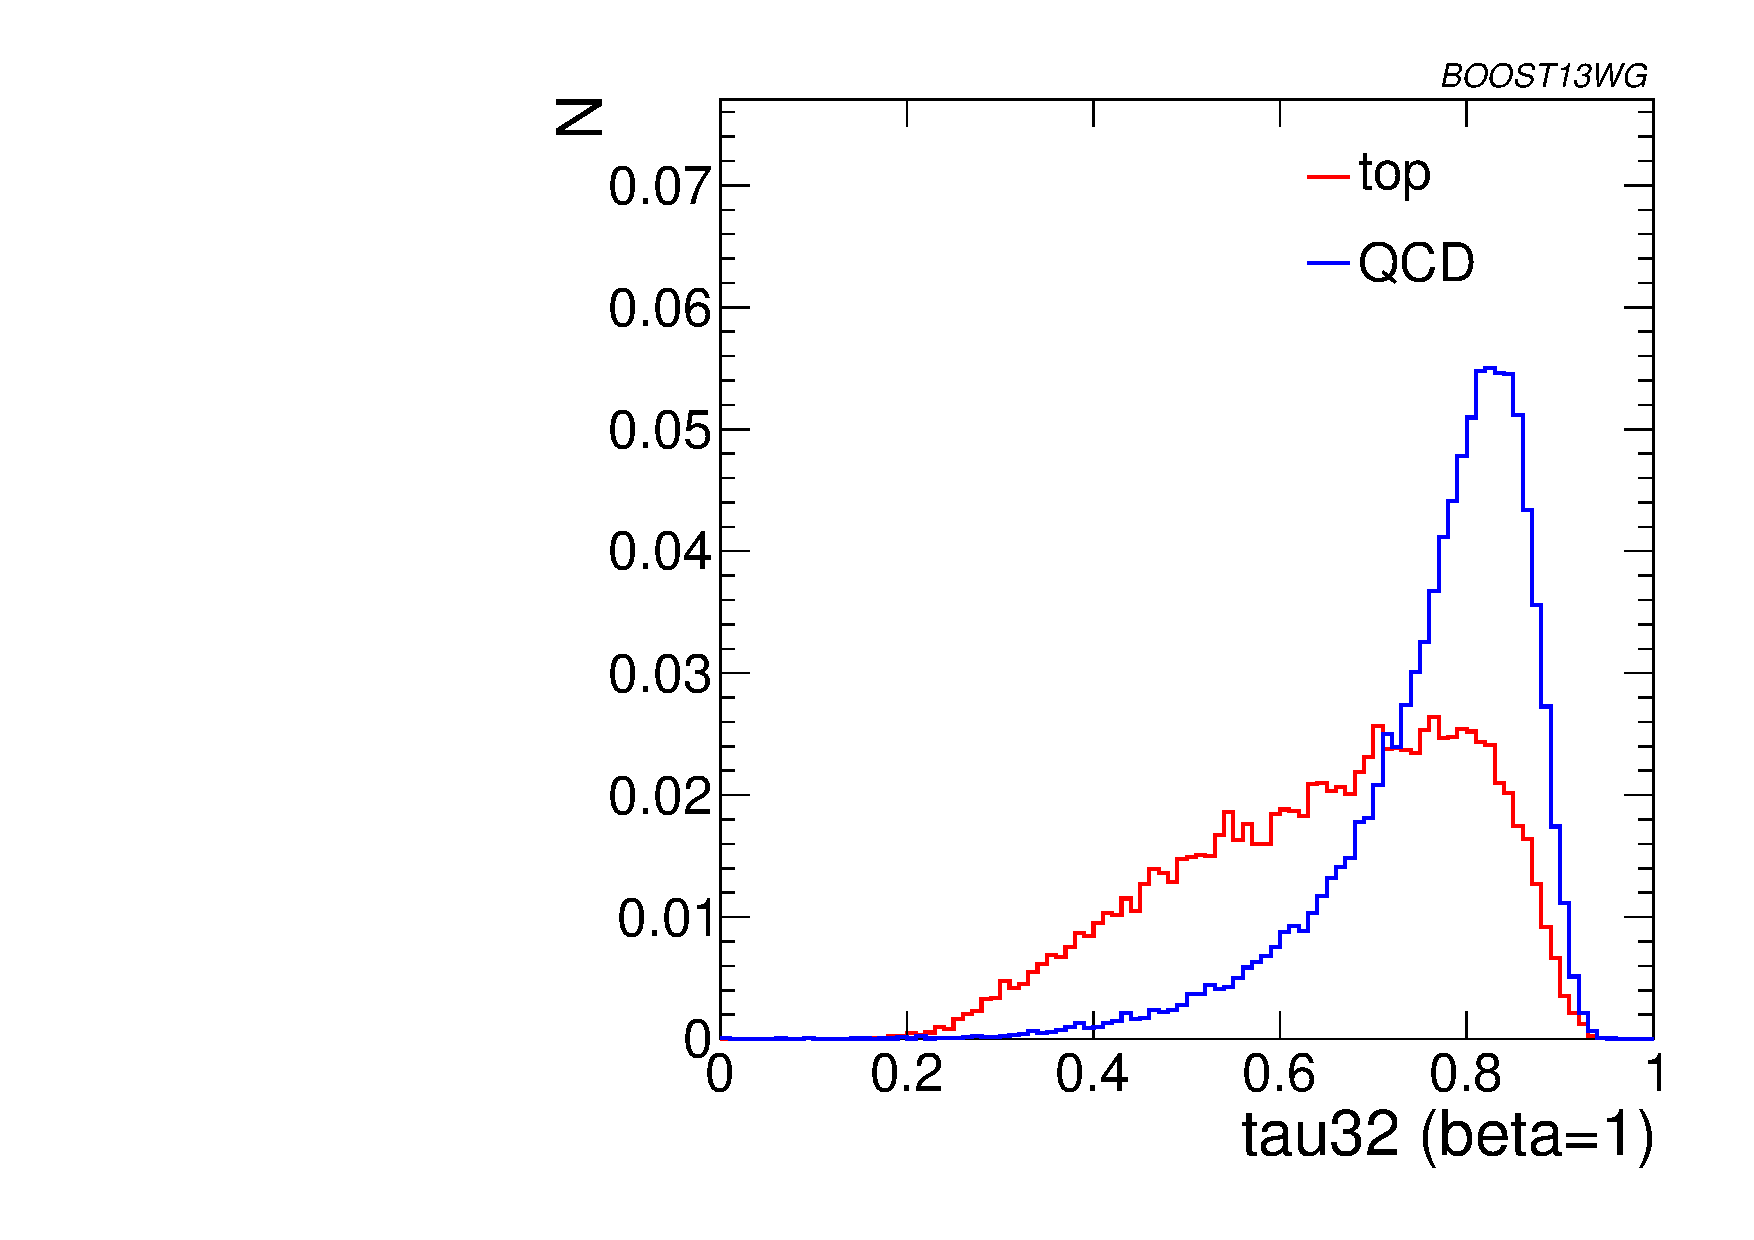
\includegraphics[width=0.245\textwidth]{./Figures/TTagging/single_variable/pT.1.5TeV.R.0.4/h_tau32b1_R_0_4.pdf}}
\subfigure[\tauthreetwo, $R=1.2$]{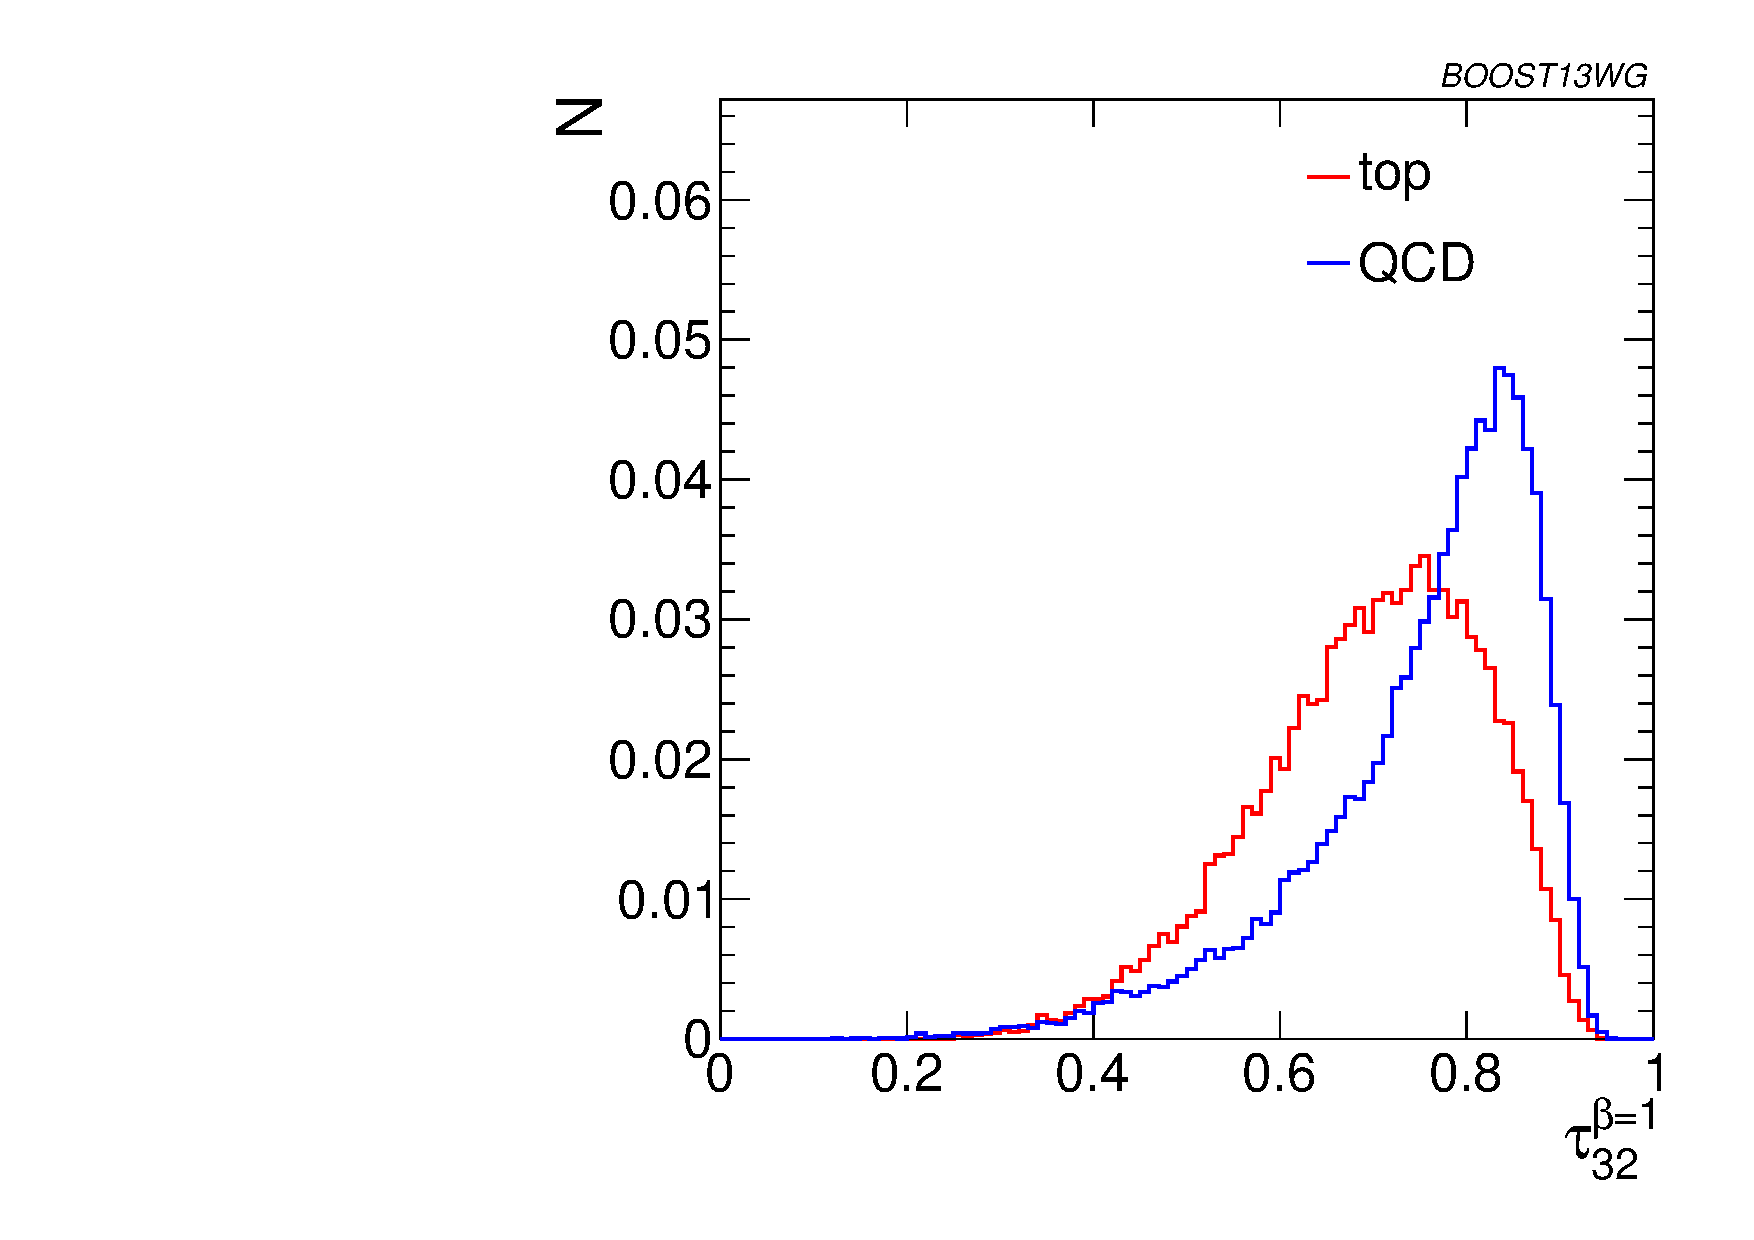
\includegraphics[width=0.245\textwidth]{./Figures/TTagging/single_variable/pT.1.5TeV.R.1.2/h_tau32b1_R_1_2.pdf}}\\
\subfigure[$\Gamma_{\rm Qjet}$, $R=0.4$]{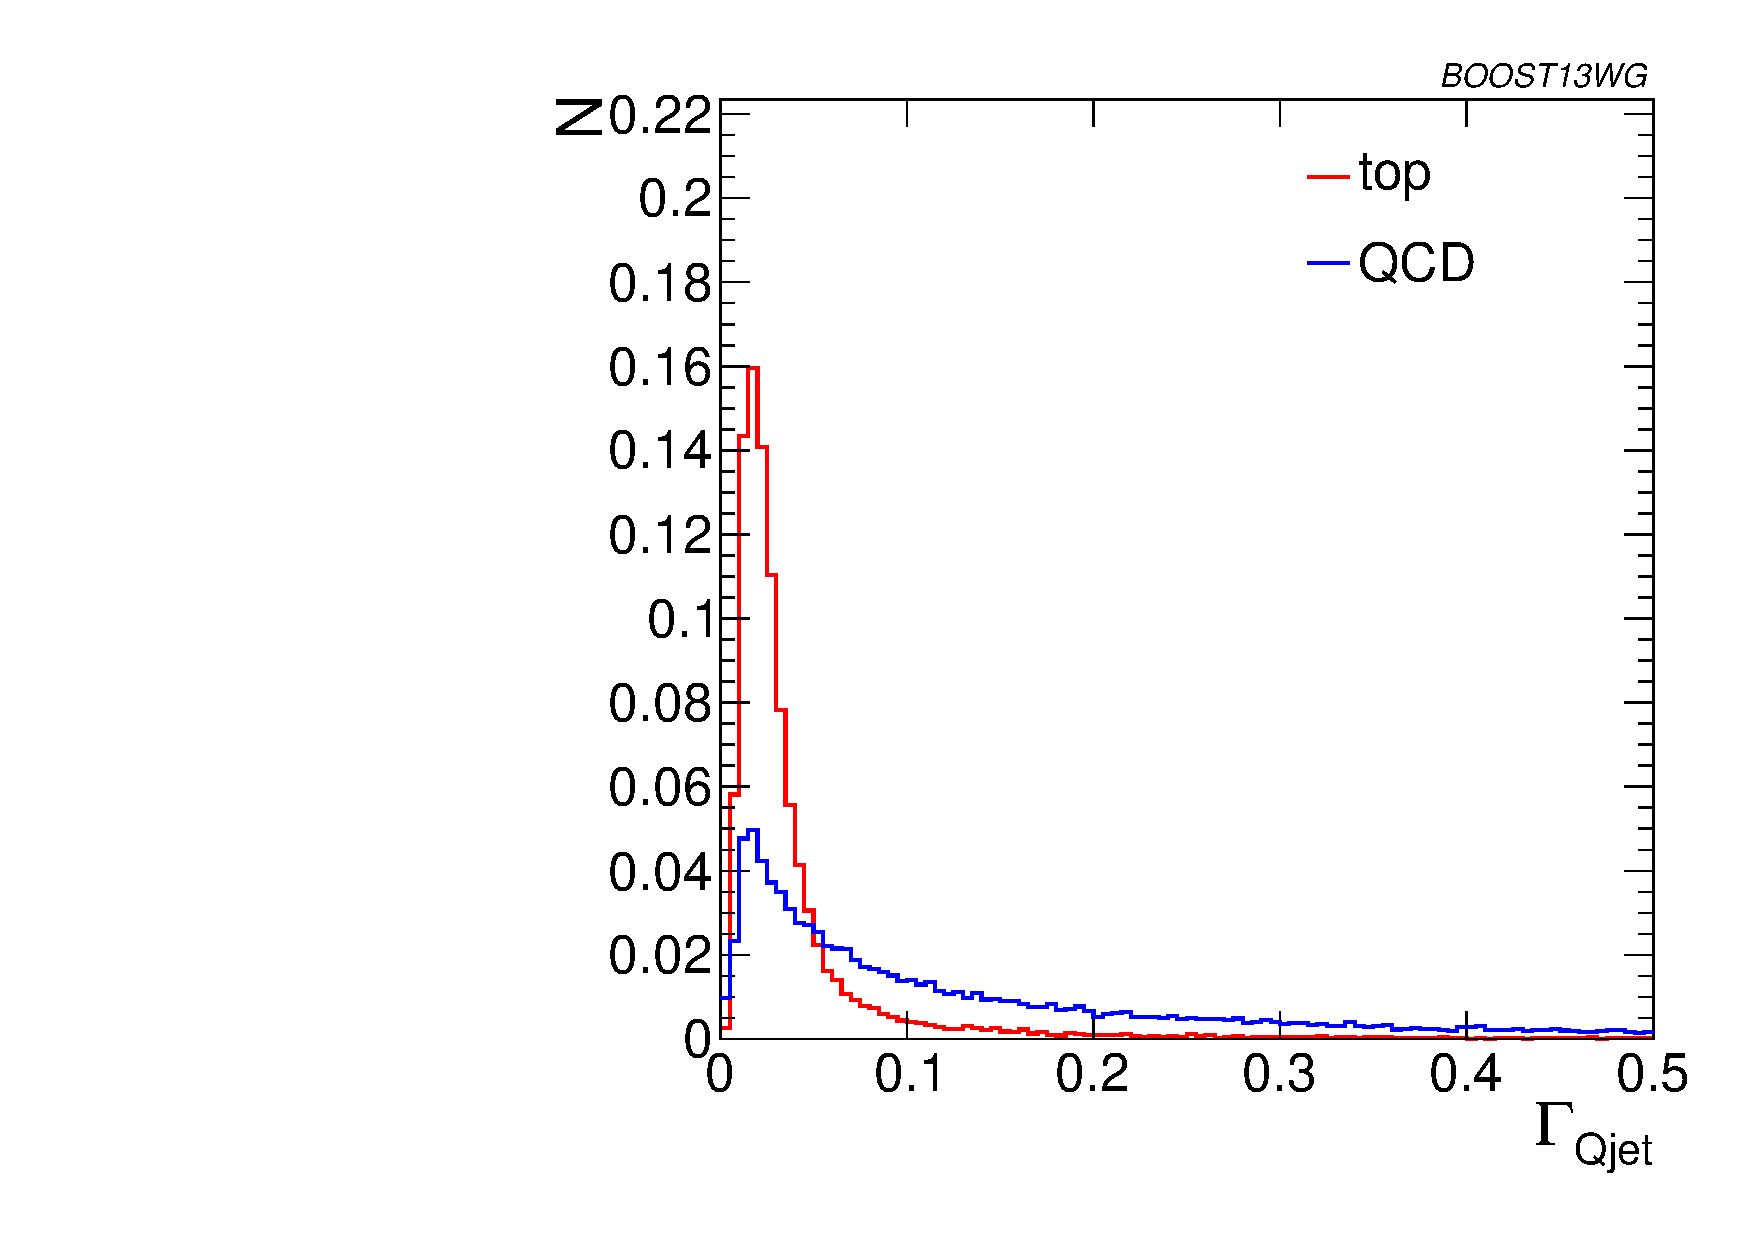
\includegraphics[width=0.245\textwidth]{./Figures/TTagging/single_variable/pT.1.5TeV.R.0.4/h_qjetVol_R_0_4.pdf}}
\subfigure[$\Gamma_{\rm Qjet}$, $R=1.2$]{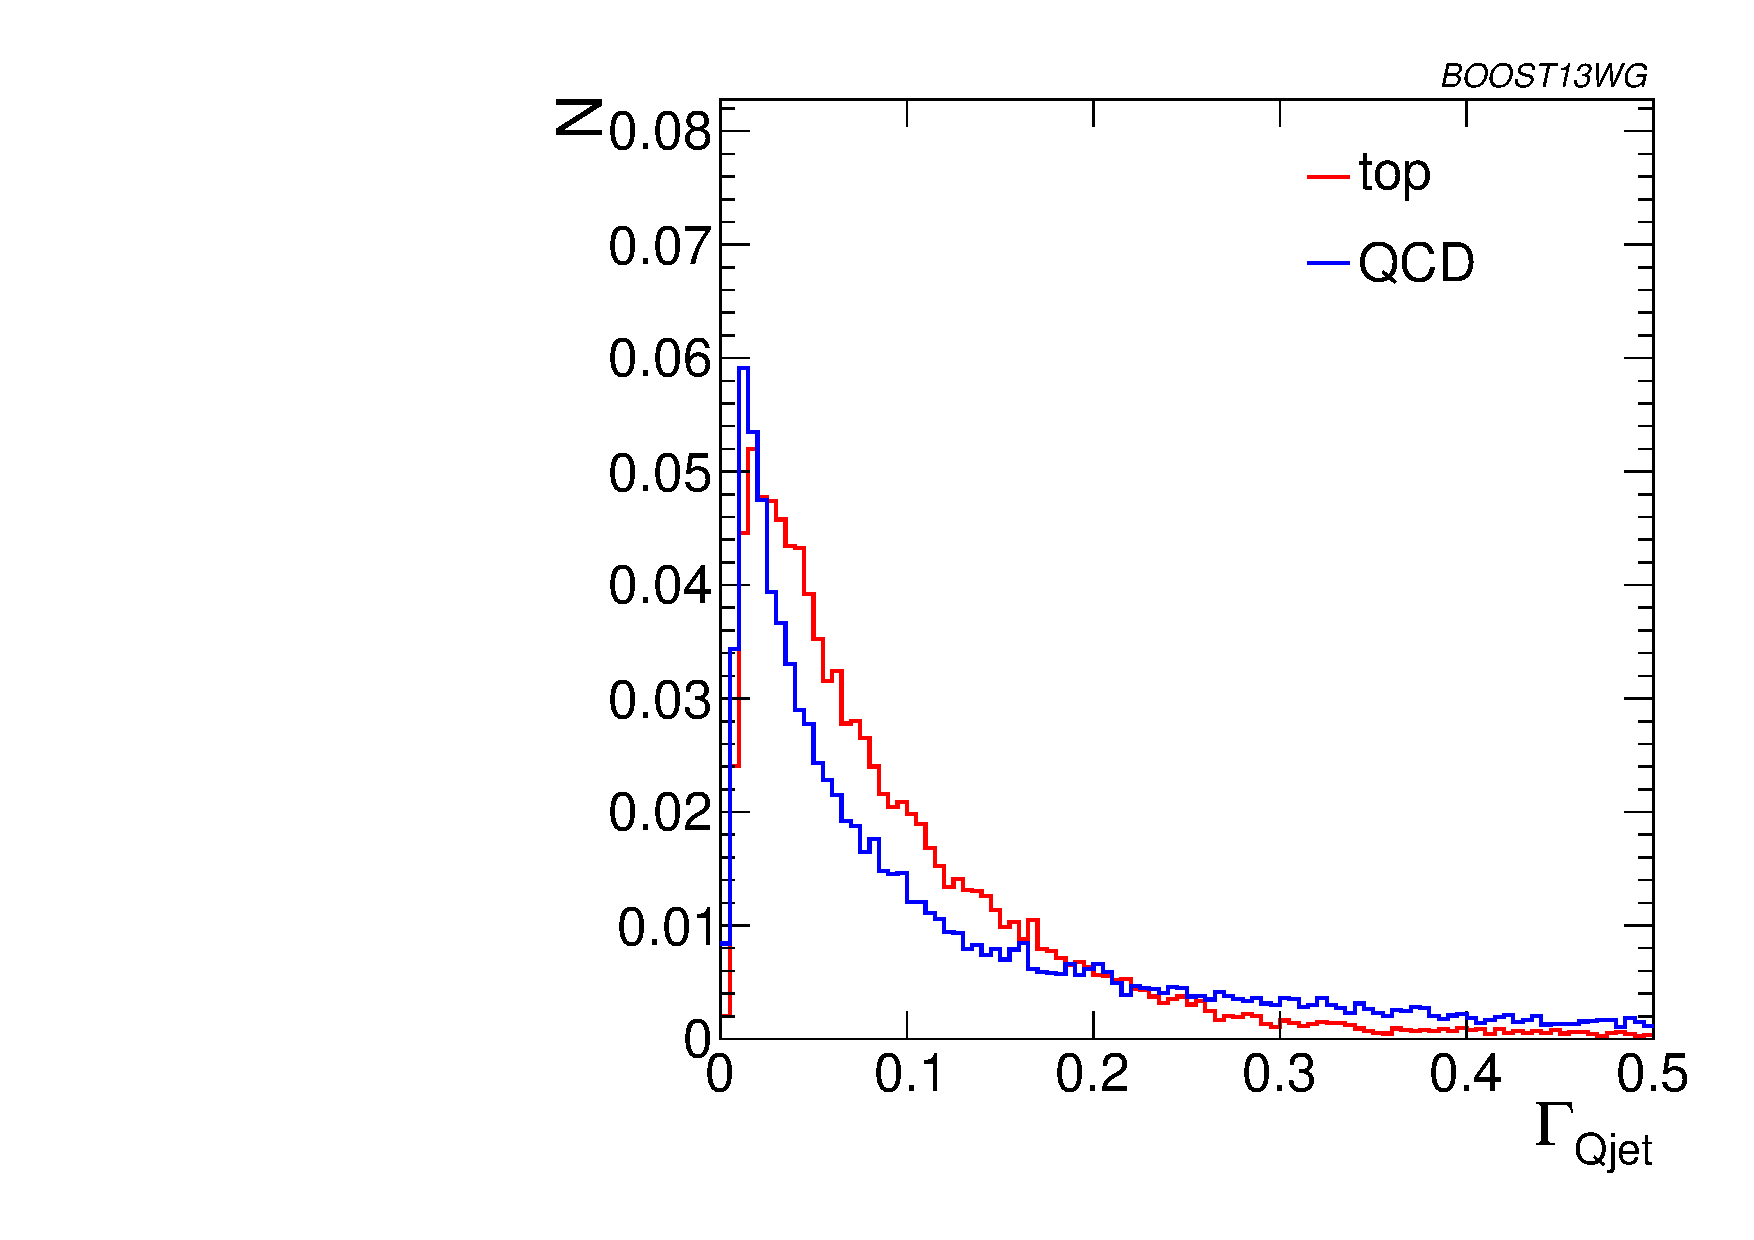
\includegraphics[width=0.245\textwidth]{./Figures/TTagging/single_variable/pT.1.5TeV.R.1.2/h_qjetVol_R_1_2.pdf}}
\caption{Comparison of various shape variables in the \pt = 1.5-1.6 \TeV bin and different values of the anti-$k_{\rm T}$ radius $R$.}
\label{fig:C_comparison_R}
\end{figure*}


\subsection{Performance of Multivariable Combinations}
We now consider various BDT combinations of the single variables considered in the last section, using the techniques described in Section~\ref{sec:multivariate}. In particular, we consider the performance of individual taggers such as the JH tagger and HEPTopTagger, which output information about the top and $W$ candidate masses and the helicity angle; for each tagger, all three output variables are combined in a BDT. For trimming and pruning, the output candidate $\wmass$ and $\topmass$ are combined in a BDT. Finally, we consider the combination of the full set of outputs of each of the above taggers/groomers with the shape variables, as well also a combination of the outputs of the HEPTopTagger and JH tagger. This allows us to determine the degree of complementary information in taggers/groomers and shape variables, as well as between the top tagging algorithms themselves. For all variables with tuneable input parameters, we scan and optimize over realistic values of such parameters, as described in Section~\ref{sec:topmethod}.



In Figure~\ref{fig:pt1000_allcompare_AKt_R08_TG}, we directly compare the performance of the HEPTopTagger, the JH tagger, trimming, and pruning, in the $\pt = 1-1.1$ TeV bin with $R=0.8$, where both \topmass~and \wmass~are used in the groomers. Generally, we find that pruning, which does not naturally incorporate subjets into the algorithm, does not perform as well as the others. Interestingly, trimming, which does include a subjet-identification step, performs comparably to the HEPTopTagger over much of the range, possibly due to the background-shaping observed in Section \ref{sec:single_variable}. By contrast, the JH tagger outperforms the other algorithms. To determine whether there is complementary information in the mass outputs from different top taggers, we also consider in Figure~\ref{fig:pt1000_allcompare_AKt_R08_TG} a multivariable combination of all of the JH and HEPTopTagger outputs. The maximum efficiency of the combined JH and HEPTopTaggers is limited, as some fraction of signal events inevitably fails either one or other of the taggers. We do see a 20-50\% improvement in performance when combining all outputs, which suggests that the different algorithms used to identify the top and $W$ for different taggers contains complementary information.

\begin{figure*}
\centering
{\includegraphics[width=0.68\textwidth]{./Figures/TTagging/multi_variable/pT.1TeV.R.0.8/Rocs_tagger_groom.pdf}}
\caption{The performance of the various taggers in the $\pt = 1-1.1$ TeV bin using the anti-\kT R=0.8 algorithm. For the groomers a BDT combination of the reconstructed \topmass~and \wmass~are used. Also shown is a multivariable combination of all of the JH and HEPTopTagger outputs. The ungroomed mass performance is shown for comparison.}
\label{fig:pt1000_allcompare_AKt_R08_TG}
\end{figure*}


In Figure~\ref{fig:pt1000_allcompare_AKt_R08_TagSh} we present the results for multivariable combinations of the top tagger outputs with and without shape variables. We see that, for both the HEPTopTagger and the JH tagger, the shape variables contain additional information uncorrelated with the masses and helicity angle, and give on average a factor 2-3 improvement in signal discrimination. We see that, when combined with the tagger outputs, both the energy correlation functions $C_2+C_3$ and the $N$-subjettiness ratios $\tau_{21}+\tau_{32}$ give comparable performance, while $\Gamma_{\rm Qjet}$ is slightly worse; this is unsurprising, as Qjets accesses shape information in a more indirect way from other shape variables. Combining all shape variables with a single top tagger provides even greater enhancement in discrimination power. We directly compare the performance of the JH and HEPTopTaggers in Figure~\ref{fig:pt1000_allcompare_AKt_R08_TagSh_Comp}. Combining the taggers with shape information nearly erases the difference between the tagging methods observed in Figure~\ref{fig:pt1000_allcompare_AKt_R08_TG}; this indicates that combining the shape information with the HEPTopTagger identifies the differences between signal and background missed by the tagger alone. This also suggests that further improvement to discriminating power may be minimal, as various multivariable combinations converge to within a factor of 20\% or so.


\begin{figure*}
\centering
\subfigure[HEPTopTagger + Shape]{\includegraphics[width=0.48\textwidth]{./Figures/TTagging/multi_variable/pT.1TeV.R.0.8/Rocs_HEP.pdf}}
\subfigure[Johns Hopkins Tagger + shape]{\includegraphics[width=0.48\textwidth]{./Figures/TTagging/multi_variable/pT.1TeV.R.0.8/Rocs_JH.pdf}}
\subfigure[HEP vs.~JH comparison (incl. shape)]{\includegraphics[width=0.48\textwidth]{./Figures/TTagging/multi_variable/pT.1TeV.R.0.8/Rocs_tagger_shape.pdf}\label{fig:pt1000_allcompare_AKt_R08_TagSh_Comp}}
\caption{The performance of BDT combinations of the JH and HepTopTagger outputs with various shape variables in the $\pt = 1-1.1$ TeV bin using the anti-\kT $R=0.8$ algorithm. Taggers are combined with the following shape variables: $\tau_{21}^{\beta=1}+\tau_{32}^{\beta=1}$, $C_{2}^{\beta=1}+C_{3}^{\beta=1}$, $\Gamma_{\rm Qjet}$, and all of the above (denoted ``shape'').}
\label{fig:pt1000_allcompare_AKt_R08_TagSh}
\end{figure*}

In Figure~\ref{fig:pt1000_allcompare_AKt_R08_GroomSh} we present the results for multivariable combinations of groomer outputs with and without shape variables. As with the tagging algorithms, combinations of groomers with shape variables improves their discriminating power; combinations with $\tau_{32}+\tau_{21}$ perform comparably to those with $C_3+C_2$, and both of these are superior to combinations with the mass volatility, $\Gamma_{\rm Qjet}$. Substantial further improvement is possible by combining the groomers with all shape variables. Not surprisingly, the taggers that lag behind in performance enjoy the largest gain in signal-background discrimination with the addition of shape variables. Once again, in Figure~\ref{fig:pt1000_allcompare_AKt_R08_GroomSh_Comp}, we find that the differences between pruning and trimming are erased when combined with shape information.

\begin{figure*}
\centering
\subfigure[Pruning + Shape]{\includegraphics[width=0.48\textwidth]{./Figures/TTagging/multi_variable/pT.1TeV.R.0.8/Rocs_prune.pdf}}
\subfigure[Trimming + Shape]{\includegraphics[width=0.48\textwidth]{./Figures/TTagging/multi_variable/pT.1TeV.R.0.8/Rocs_trim.pdf}}
\subfigure[Trim vs.~Prune comparison (incl. shape)]{\includegraphics[width=0.48\textwidth]{./Figures/TTagging/multi_variable/pT.1TeV.R.0.8/Rocs_groom_shape.pdf}\label{fig:pt1000_allcompare_AKt_R08_GroomSh_Comp}}
\caption{The performance of the BDT combinations of the trimming and pruning outputs with various shape variables in the $\pt = 1-1.1$ TeV bin using the anti-\kT $R=0.8$ algorithm. Groomer mass outputs are combined with the following shape variables: $\tau_{21}^{\beta=1}+\tau_{32}^{\beta=1}$, $C_{2}^{\beta=1}+C_{3}^{\beta=1}$, $\Gamma_{\rm Qjet}$, and all of the above (denoted ``shape'').}
\label{fig:pt1000_allcompare_AKt_R08_GroomSh}
\end{figure*}

Finally, in Figure~\ref{fig:pt1000_allcompare_AKt_R08_Final}, we compare the performance of each of the tagger/groomers when their outputs are combined with all of the shape variables considered. One can see that the discrepancies between the performance of the different taggers/groomers all but vanishes, suggesting perhaps that we are here utilising all available signal-background discrimination information, and that this is the optimal top tagging performance that could be achieved in these conditions. 

\begin{figure*}
\centering
{\includegraphics[width=0.68\textwidth]{./Figures/TTagging/multi_variable/pT.1TeV.R.0.8/Rocs_optimum.pdf}}
\caption{Comparison of the performance of the BDT combinations of all the groomer/tagger outputs with all the available shape variables in the $\pt = 1-1.1$ TeV bin using the anti-\kT R=0.8 algorithm. Tagger/groomer outputs are combined with all of the following shape variables: $\tau_{21}^{\beta=1}+\tau_{32}^{\beta=1}$, $C_{2}^{\beta=1}+C_{3}^{\beta=1}$, $\Gamma_{\rm Qjet}$.}
\label{fig:pt1000_allcompare_AKt_R08_Final}
\end{figure*}



Up to this point, we have  considered only the combined multivariable performance in the \pt =  1.0-1.1 TeV bin with jet radius $R=0.8$. We now compare the BDT combinations of tagger outputs, with and without shape variables, at different $\pt$. The taggers are optimized over all input parameters for each choice of \pt and signal efficiency. As with the single-variable study, we consider \antikt jets clustered with $R=0.8$ and compare the outcomes in the \pt = 500-600 \GeV, \pt = 1-1.1 \TeV, and \pt = 1.5-1.6 \TeV bins. The comparison of the taggers/groomers is shown in Figure~\ref{fig:ptcomparison_top}. The behaviour with \pt is qualitatively similar to the behaviour of the \topmass~variable for each tagger/groomer shown in Figure~\ref{fig:ptcomparison_singletopmass_top}; this suggests that the \pt behaviour of the taggers is dominated by the top-mass reconstruction. As before, the HEPTopTagger performance degrades slightly with increased \pt due to the background shaping effect, while the JH tagger and groomers modestly improve in performance.

In Figure~\ref{fig:ptcomparison_JH_shape}, we show the $\pt$-dependence of BDT combinations of the JH tagger output combined with shape variables. In terms of \pt dependence, we find that the curves look nearly identical to Figure~\ref{fig:ptcomparison_top_JH}:~the \pt dependence is again dominated by the top-mass reconstruction, and combining the tagger outputs with different shape variables does not substantially change this behavior. Although not shown here, the same behavior is observed for trimming and pruning. By contrast,  the \pt dependence of the HEPTopTagger ROC curves, shown in Figure~\ref{fig:ptcomparison_HEP_shape}, does change somewhat when combined with different shape variables; due to the suboptimal performance of the HEPTopTagger at high \pt, we find that combining the HEPTopTagger with $C_3^{\beta=1}$, which in Figure~\ref{fig:ptcomparison_singleshape_top_C3} is seen to have some modest improvement at high \pt, can improve its performance. Combining the HEPTopTagger with multiple shape variables gives the maximum improvement in performance at high \pt relative to at low \pt.\\

\begin{figure*}
\centering
\subfigure[HEPTopTagger]{\includegraphics[width=0.48\textwidth]{./Figures/TTagging/multi_variable/pT_compare/Rocs_HEP_pTcompare.pdf}}
\subfigure[Johns Hopkins Tagger]{\includegraphics[width=0.48\textwidth]{./Figures/TTagging/multi_variable/pT_compare/Rocs_JH_pTcompare.pdf}\label{fig:ptcomparison_top_JH}}
\subfigure[Trimming]{\includegraphics[width=0.48\textwidth]{./Figures/TTagging/multi_variable/pT_compare/Rocs_trim_mt_mw_pTcompare.pdf}}
\subfigure[Pruning]{\includegraphics[width=0.48\textwidth]{./Figures/TTagging/multi_variable/pT_compare/Rocs_prune_mt_mw_pTcompare.pdf}}
\caption{Comparison at different \pt of the performance of various top tagging/grooming algorithms using the anti-\kT $R=0.8$ algorithm. For each tagger/groomer, all output variables are combined in a BDT. }
\label{fig:ptcomparison_top}
\end{figure*}

\begin{figure*}
\centering
\subfigure[JH+$C_2^{\beta=1}$+$C_3^{\beta=1}$]{\includegraphics[width=0.48\textwidth]{./Figures/TTagging/multi_variable/pT_compare/Rocs_JH_C_pTcompare.pdf}}
\subfigure[JH+\tautwoone+\tauthreetwo]{\includegraphics[width=0.48\textwidth]{./Figures/TTagging/multi_variable/pT_compare/Rocs_JH_tau_pTcompare.pdf}}
\subfigure[JH + $\Gamma_{\rm Qjet}$]{\includegraphics[width=0.48\textwidth]{./Figures/TTagging/multi_variable/pT_compare/Rocs_JH_Qjet_pTcompare.pdf}}
\subfigure[JH + all]{\includegraphics[width=0.48\textwidth]{./Figures/TTagging/multi_variable/pT_compare/Rocs_JH_shape_pTcompare.pdf}}
\caption{Comparison at different \pt of the performance of the JH tagger using the anti-\kT $R=0.8$ algorithm, where all tagger output variables are combined in a BDT with various shape variables.}
\label{fig:ptcomparison_JH_shape}
\end{figure*}

\begin{figure*}
\centering
\subfigure[HEP+$C_2^{\beta=1}$+$C_3^{\beta=1}$]{\includegraphics[width=0.48\textwidth]{./Figures/TTagging/multi_variable/pT_compare/Rocs_HEP_C_pTcompare.pdf}}
\subfigure[HEP+\tautwoone+\tauthreetwo]{\includegraphics[width=0.48\textwidth]{./Figures/TTagging/multi_variable/pT_compare/Rocs_HEP_tau_pTcompare.pdf}}
\subfigure[HEP + $\Gamma_{\rm Qjet}$]{\includegraphics[width=0.48\textwidth]{./Figures/TTagging/multi_variable/pT_compare/Rocs_HEP_Qjet_pTcompare.pdf}}
\subfigure[HEP + all]{\includegraphics[width=0.48\textwidth]{./Figures/TTagging/multi_variable/pT_compare/Rocs_HEP_shape_pTcompare.pdf}}
\caption{Comparison at different \pt of the performance of the HEPTopTagger using the anti-\kT $R=0.8$ algorithm,  where all tagger output variables are combined in a BDT with various shape variables.}
\label{fig:ptcomparison_HEP_shape}
\end{figure*}



In Figure ~\ref{fig:Rcomparison_top} we compare the BDT combinations of tagger outputs, with and without shape variables, at different jet radius $R$ in the \pt = 1.5-1.6 \TeV bin. The taggers are optimized over all input parameters for each choice of $R$ and signal efficiency. We find that, for all taggers and groomers, the performance is always best at small $R$; the choice of $R$ is sufficiently large to admit the full top quark decay at such high \pt, but is small enough to suppress contamination from additional radiation. This is not altered when the taggers are combined with shape variables. For example, in Figure~\ref{fig:Rcomparison_JH_shape} is shown the dependence on $R$ of the JH tagger when combined with shape variables, where one can see that the $R$-dependence is identical for all combinations. The same holds true for the HEPTopTagger, trimming, and pruning.

\begin{figure*}
\centering
\subfigure[HEPTopTagger]{\includegraphics[width=0.48\textwidth]{./Figures/TTagging/multi_variable/R_compare/Rocs_HEP_Rcompare.pdf}}
\subfigure[Johns Hopkins Tagger]{\includegraphics[width=0.48\textwidth]{./Figures/TTagging/multi_variable/R_compare/Rocs_JH_Rcompare.pdf}}
\subfigure[Trimming]{\includegraphics[width=0.48\textwidth]{./Figures/TTagging/multi_variable/R_compare/Rocs_trim_mt_mw_Rcompare.pdf}}
\subfigure[Pruning]{\includegraphics[width=0.48\textwidth]{./Figures/TTagging/multi_variable/R_compare/Rocs_prune_mt_mw_Rcompare.pdf}}
\caption{Comparison at different radii of the performance of various top tagging/grooming algorithms with \pt = 1.5-1.6 TeV. For each tagger/groomer, all output variables are combined in a BDT.}
\label{fig:Rcomparison_top}
\end{figure*}

\begin{figure*}
\centering
\subfigure[JH+$C_2^{\beta=1}$+$C_3^{\beta=1}$]{\includegraphics[width=0.48\textwidth]{./Figures/TTagging/multi_variable/R_compare/Rocs_JH_C_Rcompare.pdf}}
\subfigure[JH+\tautwoone+\tauthreetwo]{\includegraphics[width=0.48\textwidth]{./Figures/TTagging/multi_variable/R_compare/Rocs_JH_tau_Rcompare.pdf}}
\subfigure[JH + $\Gamma_{\rm Qjet}$]{\includegraphics[width=0.48\textwidth]{./Figures/TTagging/multi_variable/R_compare/Rocs_JH_Qjet_Rcompare.pdf}}
\subfigure[JH + all]{\includegraphics[width=0.48\textwidth]{./Figures/TTagging/multi_variable/R_compare/Rocs_JH_shape_Rcompare.pdf}}
\caption{Comparison at different radii of the performance of the JH tagger in the \pt = 1.5-1.6 TeV bin, where all tagger output variables are combined in a BDT  with various shape variables}
\label{fig:Rcomparison_JH_shape}
\end{figure*}

\subsection{Performance at Sub-Optimal Working Points}

Up until now, we have re-optimized our tagger and groomer parameters for each $\pt$, $R$, and signal efficiency working point. In reality, experiments will choose a finite set of working points to use. When this is taken into account, how will the top-tagging performance compare to the optimal results already shown? To address this concern, we replicate our analyses, but optimize the top taggers only for a single $\pt$ bin, single jet radius $R$, or single signal efficiency, and subsequently apply the same parameters to other scenarios. This allows us to determine the extent to which re-optimization is necessary to maintain the high signal-to-background discrimination power seen in the top-tagging algorithms we studied. In this section, we focus on the taggers and groomers, and their combination with shape variables, as the shape variables alone typically do not have any input parameters to optimize.

\noindent {\bf Optimizing at a single \pt:}
We show in Figure~\ref{fig:ptcomparison_singletopmass_top_optOnce} the performance of the reconstructed top mass for the \pt = 0.6-0.7 \TeV and \pt = 1.0-1.1 \TeV bins, with all input parameters optimized to the \pt = 1.5-1.6 \TeV bin (and $R=0.8$ throughout). This is normalized to the performance using the optimized tagger inputs at each \pt. The performance degradation is at the level of 20-30\% (at maximum 50\%) when the high-\pt optimized inputs are used at other momenta,
with trimming and the Johns Hopkins tagger degrading the most. The jagged behaviour of the points is due to the finite resolution of the scan. We also observe a particular effect associated with using suboptimal taggers:~since taggers sometimes fail to return a top candidate, parameters optimized for a particular signal efficiency $\varepsilon_{\rm sig}$ at \pt = 1.5-1.6 \TeV may not return enough signal candidates to reach the same efficiency at a different $\pt$. Consequently, no point appears for that $\pt$ value. This is not often a practical concern, as the largest gains in signal discrimination and significance are for smaller values of $\varepsilon_{\rm sig}$, but it may be an important effect to consider when selecting benchmark tagger parameters and signal efficiencies.

\begin{figure*}
\centering
\subfigure[HEPTopTagger $m_t$]{\includegraphics[width=0.48\textwidth]{./Figures/TTagging/single_variable/pT_compare/Rocs_HEP_mt_pTcompare_optOnce.pdf}}
\subfigure[Johns Hopkins Tagger $m_t$]{\includegraphics[width=0.48\textwidth]{./Figures/TTagging/single_variable/pT_compare/Rocs_JH_mt_pTcompare_optOnce.pdf}}
\subfigure[Pruning $m_t$]{\includegraphics[width=0.48\textwidth]{./Figures/TTagging/single_variable/pT_compare/Rocs_prune_pTcompare_optOnce.pdf}}
\subfigure[Trimming $m_t$]{\includegraphics[width=0.48\textwidth]{./Figures/TTagging/single_variable/pT_compare/Rocs_trim_pTcompare_optOnce.pdf}}
\caption{Comparison of the top mass performance of different taggers at different \pt using the anti-\kT $R=0.8$ algorithm. The tagger inputs are set to the optimum value for \pt = 1.5-1.6 \TeV, and the performance is normalized to the performance using the optimized tagger inputs at each \pt.}
\label{fig:ptcomparison_singletopmass_top_optOnce}
\end{figure*}

The degradation in performance is more pronounced for the BDT combinations of the full tagger outputs, shown in Figure~\ref{fig:ptcomparison_top_optOnce}. This is true particularly at very low signal efficiency, where the optimization of inputs picks out a cut on the tail of some distribution that depends precisely on the $\pt$/$R$ of the jet. Once again, trimming and the Johns Hopkins tagger degrade more markedly.  Similar behavior holds for the BDT combinations of tagger outputs plus all shape variables.\\

\begin{figure*}
\centering
\subfigure[HEPTopTagger]{\includegraphics[width=0.48\textwidth]{./Figures/TTagging/multi_variable/pT_compare/Rocs_HEP_pTcompare_optOnce.pdf}}
\subfigure[Johns Hopkins Tagger]{\includegraphics[width=0.48\textwidth]{./Figures/TTagging/multi_variable/pT_compare/Rocs_JH_pTcompare_optOnce.pdf}}
\subfigure[Pruning]{\includegraphics[width=0.48\textwidth]{./Figures/TTagging/multi_variable/pT_compare/Rocs_prune_mt_mw_pTcompare_optOnce.pdf}}
\subfigure[Trimming]{\includegraphics[width=0.48\textwidth]{./Figures/TTagging/multi_variable/pT_compare/Rocs_trim_mt_mw_pTcompare_optOnce.pdf}}
\caption{Comparison of tagger performance at different \pt using the \antikt $R=0.8$ algorithm. For each tagger/groomer, all output variables are combined in a BDT, and the tagger inputs are set to the optimum value for \pt = 1.5-1.6 \TeV. The performance is normalized to the performance using the optimized tagger inputs at each \pt.}
\label{fig:ptcomparison_top_optOnce}
\end{figure*}


\noindent {\bf Optimizing at a single $R$:}
In Figure~\ref{fig:Rcomparison_singletopmass_top_optOnce}, we show the performance of the reconstructed top mass for $R=0.4$ and 0.8, with all input parameters optimized to $R=1.2$ TeV bin (and \pt = 1.5-1.6 \TeV throughout). This is normalized to the performance using the optimized tagger inputs at each $R$. While the performance of each variable degrades at small $\varepsilon_{\rm sig}$ compared to the optimized search, the HEPTopTagger fares the worst. It is not surprising that a tagger whose top mass reconstruction is susceptible to background-shaping at large $R$ and $\pt$ would require a more careful optimization of parameters to obtain the best performance.

\begin{figure*}
\centering
\subfigure[HEPTopTagger $m_t$]{\includegraphics[width=0.48\textwidth]{./Figures/TTagging/single_variable/R_compare/Rocs_HEP_mt_Rcompare_optOnce.pdf}}
\subfigure[Johns Hopkins Tagger $m_t$]{\includegraphics[width=0.48\textwidth]{./Figures/TTagging/single_variable/R_compare/Rocs_JH_mt_Rcompare_optOnce.pdf}}
\subfigure[Pruning $m_t$]{\includegraphics[width=0.48\textwidth]{./Figures/TTagging/single_variable/R_compare/Rocs_prune_Rcompare_optOnce.pdf}}
\subfigure[Trimming $m_t$]{\includegraphics[width=0.48\textwidth]{./Figures/TTagging/single_variable/R_compare/Rocs_trim_Rcompare_optOnce.pdf}}
\caption{Comparison of the top mass performance of different taggers at different $R$ in the \pt = 1.5-1.6 \TeV bin. The tagger inputs are set to the optimum value for $R=1.2$, and the performance is normalized to the performance using the optimized tagger inputs at each $R$.}
\label{fig:Rcomparison_singletopmass_top_optOnce}
\end{figure*}

The same holds true for the BDT combinations of the full tagger outputs, shown in Figure~\ref{fig:Rcomparison_top_optOnce}. The performance for the sub-optimal taggers is still within an $O(1)$ factor of the optimized performance, and the HEPTopTagger performs better with the combination of all of its outputs relative to the performance with just \topmass. The same behaviour holds for the BDT combinations of tagger outputs and shape variables. \\


\begin{figure*}
\centering
\subfigure[HEPTopTagger]{\includegraphics[width=0.48\textwidth]{./Figures/TTagging/multi_variable/R_compare/Rocs_HEP_Rcompare_optOnce.pdf}}
\subfigure[Johns Hopkins Tagger]{\includegraphics[width=0.48\textwidth]{./Figures/TTagging/multi_variable/R_compare/Rocs_JH_Rcompare_optOnce.pdf}}
\subfigure[Pruning]{\includegraphics[width=0.48\textwidth]{./Figures/TTagging/multi_variable/R_compare/Rocs_prune_mt_mw_Rcompare_optOnce.pdf}}
\subfigure[Trimming]{\includegraphics[width=0.48\textwidth]{./Figures/TTagging/multi_variable/R_compare/Rocs_trim_mt_mw_Rcompare_optOnce.pdf}}
\caption{Comparison of tagger performance at different $R$ in \pt = 1.5-1.6 \TeV bin. For each tagger/groomer, all output variables are combined in a BDT, and the tagger inputs are set to the optimum value for $R=1.2$, and the performance is normalized to the performance using the optimized tagger inputs at each $R$.}
\label{fig:Rcomparison_top_optOnce}
\end{figure*}


\noindent {\bf Optimizing at a single efficiency:}
The strongest assumption we have made so far is that the taggers can be re-optimized for each signal efficiency point. This is useful for making a direct comparison of the power of different top-tagging algorithms, but is not particularly practical for LHC analyses. We now consider the scenario in which the tagger inputs are optimized once, in the $\varepsilon_{\rm sig}=0.3$-$0.35$ bin, and then used for all signal efficiencies. We do this in the  \pt = 1.0-1.1 \TeV bin and with $R=0.8$.

The performance of each tagger, normalized to its performance optimized in each signal efficiency bin, is shown in Figure~\ref{fig:single_variable_ROC_eps0_35} for cuts on the top mass and $W$ mass, and in Figure~\ref{fig:pt1000_allcompare_AKt_R08_eps0_35} for BDT combinations of tagger outputs and shape variables. In both plots, it is apparent that optimizing the taggers in the $\varepsilon_{\rm sig}=0.3$-$0.35$ efficiency bin gives comparable performance over efficiencies ranging from 0.2-0.5, although performance degrades at substantially different signal efficiencies. Pruning appears to give especially robust signal-background discrimination without re-optimization, most likely due to the fact that there are no absolute distance or \pt scales that appear in the algorithm. Figures~\ref{fig:single_variable_ROC_eps0_35} and~\ref{fig:pt1000_allcompare_AKt_R08_eps0_35} suggest that, while optimization at all signal efficiencies is a useful tool for comparing different algorithms, it is not crucial to achieve good top-tagging performance in experiments.

\begin{figure*}
\centering
\includegraphics[width=0.49\textwidth]{./Figures/TTagging/single_variable/pT.1TeV.R.0.8/Rocs_top_mass_eff0_35.pdf}
\caption{Comparison of  top-tagging performance with $\topmass$ in the $\pt= 1-1.1$ GeV bin using the anti-\kT, $R=0.8$ algorithm. The inputs for each tagger are optimized for the $\varepsilon_{\rm sig}=0.3-0.35$ bin, and the performance is normalized to the performance using the optimized tagger inputs at each $\varepsilon_{\rm sig}$.}
\label{fig:single_variable_ROC_eps0_35}
\end{figure*}

\begin{figure*}
\centering
\subfigure[Tagger-Groomer comparison]{\includegraphics[width=0.48\textwidth]{./Figures/TTagging/multi_variable/pT.1TeV.R.0.8/Rocs_tagger_groom_eff0_35.pdf}}
\subfigure[HEPTopTagger + Shape]{\includegraphics[width=0.48\textwidth]{./Figures/TTagging/multi_variable/pT.1TeV.R.0.8/Rocs_HEP_eff0_35.pdf}}
\subfigure[Johns Hopkins Tagger + shape]{\includegraphics[width=0.48\textwidth]{./Figures/TTagging/multi_variable/pT.1TeV.R.0.8/Rocs_JH_eff0_35.pdf}}
\subfigure[HEP vs.~JH comparison (incl. shape)]{\includegraphics[width=0.48\textwidth]{./Figures/TTagging/multi_variable/pT.1TeV.R.0.8/Rocs_tagger_shape_eff0_35.pdf}}
\subfigure[Pruning + Shape]{\includegraphics[width=0.48\textwidth]{./Figures/TTagging/multi_variable/pT.1TeV.R.0.8/Rocs_prune_eff0_35.pdf}}
\subfigure[Trimming + Shape]{\includegraphics[width=0.48\textwidth]{./Figures/TTagging/multi_variable/pT.1TeV.R.0.8/Rocs_trim_eff0_35.pdf}}
\subfigure[Trim vs.~Prune comparison (incl. shape)]{\includegraphics[width=0.48\textwidth]{./Figures/TTagging/multi_variable/pT.1TeV.R.0.8/Rocs_groom_shape_eff0_35.pdf}}
\subfigure[Comparison of all Tagger+Shape]{\includegraphics[width=0.48\textwidth]{./Figures/TTagging/multi_variable/pT.1TeV.R.0.8/Rocs_optimum_eff0_35.pdf}}
\caption{The BDT combinations in the $\pt = 1-1.1$ TeV bin using the anti-\kT $R=0.8$ algorithm. Taggers are combined with the following shape variables: $\tau_{21}^{\beta=1}+\tau_{32}^{\beta=1}$, $C_{2}^{\beta=1}+C_{3}^{\beta=1}$, $\Gamma_{\rm Qjet}$, and all of the above (denoted ``shape''). The inputs for each tagger are optimized for the $\varepsilon_{\rm sig}=0.3-0.35$ bin, and the performance is normalized to the performance using the optimized tagger inputs at each $\varepsilon_{\rm sig}$.}
\label{fig:pt1000_allcompare_AKt_R08_eps0_35}
\end{figure*}




\subsection{Conclusions}


We have studied the performance of various jet substructure variables, groomed masses, and top taggers to study the performance of top tagging with different \pt and jet radius parameters. At each \pt, $R$, and signal efficiency working point, we optimize the parameters for those variables with tuneable inputs. Overall, we have found that these techniques, individually and in combination, continue to perform well at high $\pt$, at least at the particle-level, which is important for future LHC running. In general, the John Hopkins tagger performs best, while jet grooming algorithms under-perform relative to the best top taggers due to the lack of an optimized $W$-identification step. 
Tagger performance can be improved by a further factor of 2-4 through combination with jet substructure variables such as $\tau_{32}$, $C_3$, and $\Gamma_{\rm Qjet}$. When combined with jet substructure variables, the performance of various groomers and taggers becomes very comparable, suggesting that, taken together, the variables studied are sensitive to nearly all of the physical differences between top and QCD jets at particle-level. A small improvement is also found by combining the Johns Hopkins and HEPTopTaggers, indicating that different taggers are not fully correlated. The degree to which these findings continue to hold under more realistic pile-up and detector configurations is, however, not addressed in this analysis and left to future study.

Comparing results at different \pt and $R$, top-tagging performance is generally better at smaller $R$ due to less contamination from uncorrelated radiation. Similarly, most variables perform better at larger $\pt$ due to the higher degree of collimation of radiation. Some variables fare worse at higher $\pt$, such as the $N$-subjettiness ratio $\tau_{32}$ and the Qjet mass volatility $\Gamma_{\rm Qjet}$, as higher-$\pt$ QCD jets have more and harder emissions that fake the top-jet substructure. The HEPTopTagger is also worse at high $\pt$ due to the tendency of the tagger to shape backgrounds around the top mass. This is unsurprising, given that the HepTopTagger was specifically designed for a lower \pT range than that considered here. The \pt- and $R$-dependence of the multivariable combinations is dominated by the \pt- and $R$-dependence of the top mass reconstruction component of the tagger/groomer.

Finally, we consider the performance of various tagger and jet substructure variable combinations under the more realistic assumption that the input parameters are only optimized at a single $\pt$, $R$, or signal efficiency, and then the same inputs are used at other working points. Remarkably, the performance of all variables is typically within a factor of 2 of the fully optimized inputs, suggesting that while optimization can lead to substantial gains in performance, the general behavior found in the fully optimized analyses extends to more general applications of each variable. In particular, the performance of pruning typically varies the least when comparing sub-optimal working points to the fully optimized tagger due to the scale-invariant nature of the pruning algorithm.
